\section{Standard Model and the Higgs mechanism}
\label{sec::SM_appendix}

The electric charge $Q$ is the generator that the massless photon couples to. It is an invariant quantity and is defined as \cite{zee2003quantum}

\begin{equation}
Q = T_3 + \frac{1}{2}Y
\label{eqn:electricchargegenerator}
\end{equation}

Here $T$ denotes the generator of the isospin symmetry group $SU(2)$ and $Y$ denotes the generator of hypercharge symmetry group $U(1)_Y$. The $SU(2)$ generators obey the Lie algebra
\begin{equation}
[T^a, T^b] = i\varepsilon^{abc}T_c.
\label{eqn:su2liealgebr}
\end{equation}

where $\varepsilon^{abc}$ is the antisymmetric Levi-Civita symbol. Under the fundamental representation the generators of $SU(2)$  becomes the Pauli matrices: $T_a = \sigma_a/2$ \cite{roubillard2005th}. The Standard Model Lagrangian is \cite{noteskooijman11}.

\begin{equation}
\mathcal L_{SM} = \mathcal L_{kinetic} + \mathcal L_{Higgs} + \mathcal L_{Yukawa},
\label{eqn:SMLagrangian}
\end{equation}
with the kinetic term describing the dynamics of the spinor fields $\psi$
\begin{equation}
\mathcal L_{kinetic} = i\overline{\psi}(\partial^\mu\gamma_\mu)\psi,
\label{eqn:SMLkinetic}
\end{equation}
with $\overline{\psi} \equiv \psi^\dag\gamma^0$, and $\psi$ the three fermion generations which will be later represented by an index $i$. 

The gauge invariance under the three symmetry group is imposed by replacing the derivative with a covariant derivative obtaining the fields of the interactions corresponding to the symmetry groups:

\begin{equation}
\mathcal L_{kinetic} =  i\overline{\psi}(D^\mu\gamma_\mu)\psi \\;
\label{eqn:newSMLkinetic}
\end{equation}
with
\begin{equation}
D^\mu = \partial^\mu + i\frac{g_s}{2}G^\mu_aL_a + i\frac{g}{2}W^\mu_b\sigma_b+i\frac{g'}{2}B^\mu Y,
\label{eqn:SMcovariant}
\end{equation}
where $L_a$ are the Gell-Mann matrices which gives the generators of $SU(3)$ so $t_a \equiv L_a/2$, $\sigma_b$ are the Pauli matrices which gives the generators of $SU(2)$ $T_a \equiv i\sigma_b/2$, $g_s$, $g$, and $g'$ are respectively the strong $SU(3)$, the electroweak isospin $SU(2)$, and hypercharge $U(1)$ couplings and $G^\mu_a$, $W^\mu_b$, and $B^\mu$ are respectively the eight gluon fields, the three weak interaction bosons that form a triplet, and the single hypercharge boson.

The fermion fields $\psi$ then transform as 
\begin{equation}
\psi(x) \to \mathrm{e}^{i\pi^a\sigma_a/2}\mathrm{e}^{iY\beta(x)}\psi(x),
\label{eqn:phitransformsagain}
\end{equation}
with $Y$ the generator of $U(1)$ and $\pi^a$ the parameters of the $SU(2)$ transformations. The abelian $U(1)_Y$ and the nonabelian $SU(2)_L$ have the Yang-Mills terms $\mathcal{L}_{gauge} = -\frac{1}{4}(G^a_{\mu\nu}G^{a\mu\nu} + H_{\mu\nu}H^{\mu\nu})$ with $H_{\mu\nu} = \partial_\mu B_{\nu} -\partial_\nu B_\mu$ and $G^a_{\mu\nu}= \partial_\mu W^a_\nu -\partial_\nu W^a_\mu + g\varepsilon^{abc}W^b_\mu W^c_\mu$, from which it can be seen that the gauge bosons self-interact \cite{roubillard2005th}.

The $SU(2)_L \times U(1)_Y$ gauge theory is the partially unified theory of the weak and electromagnetic interactions of Glashow, Weinberg, and Salam \cite{peskin1995introduction}. Through spontaneous breaking of the symmetry of these groups to $U(1)_{EM}$, the electromagnetic gauge group, the $W$ and $Z$ bosons gain mass. This works again according to the Higgs mechanism of the previous section; for this to occur, first a Higgs scalar field is to be added to the Lagrangian \cite{quigg1983gauge}:
\begin{equation}
\mathcal L_{Higgs} = (D_\mu\phi)^\dag(D^\mu\phi) - \mu^2\phi^\dag\phi - \lambda(\phi^\dag\phi)^2,
\label{eqn:SMLHiggs}
\end{equation}
from which the mass of the bosons comes from the interaction term (which contains a covariant derivative) after spontaneous symmetry breaking. This is a generalization of the abelian Higgs model to a nonabelian gauge group. Each fermion generation is made of five different representations \cite{peskin1995introduction}:

\begin{enumerate}
	\label{enum:hypercharges}
	\item Left-handed quarks $Q^I_{Li}$, which are a triplet under $SU(3)$, a doublet $\left(\begin{array}{c} u \\ d \end{array} \right)^I_{Li}$ under $SU(2)$, and have hypercharge $Y = \frac{1}{3}$;
	\item Right handed ``up'' quarks (i.e. up, charm, top)  $u^I_{Ri}$, which are an $SU(3)$ triplet, $SU(2)$ singlet, and have hypercharge $Y = \frac{4}{3}$;
	\item Right handed ``down'' quarks (i.e. down, strange, bottom)  $d^I_{Ri}$, which are an $SU(3)$ triplet, $SU(2)$ singlet, and have hypercharge $Y = \frac{-2}{3}$;
	\item Left-handed leptons  $L^I_{Li}$, which are an $SU(3)$ singlet, $SU(2)$ doublet  $\left(\begin{array}{c} \nu \\ e \end{array} \right)^I_{Li}$, and have hypercharge $Y = -1$;
	\item Right-handed ``electron'' leptons $L^I_{Ri}$, which are an $SU(3)$ singlet, $SU(2)$ singlet, and have hypercharge $Y = -2$. The name is given because only the electron, muon, and tau are included; right-handed neutrinos are not.
\end{enumerate}

Contrary to experimental evidence the mass of the right-handed neutrinos is comparable their lepton counterpart, therefore they have not been included in the list.

\subsection{The Bosonic Masses}
\label{section:bosonicmasses}
In the case $\phi(x)$  takes a vacuum expectation value of $v =  \sqrt{\frac{-\mu^2}{|\lambda|}}$, which corresponds to the minimum of the potential $V(\phi^\dag\phi) = \mu^2(\phi^\dag\phi) + |\lambda|(\phi^\dag\phi)^2$ only if $\mu^2<0$:

\begin{equation}
\left( \begin{array}{c}
\phi^+ \\
\phi^0 \end{array} \right) \rightarrow \frac{1}{\sqrt{2}}\left( \begin{array}{c}
0 \\
v \end{array} \right) \equiv \left<\phi\right>_0.
\label{eqn:vevphi}
\end{equation}

For this case , where $\left< 0 | \phi | 0\right> \neq 0$,  electroweak symmetry is spontaneously broken: $SU(2)_L\otimes U(1)_Y \to U(1)_{EM}$.
The generators of $SU(2)_L \otimes U(1)_Y$ do not leave this vacuum where v is assumed invariant. The generator corresponding to electric charge, however, does leave the vacuum invariant, so that the photon associated with electric charge will not acquire a mass \cite{quigg1983gauge}.

It is possible now to write $\phi$ in terms of fluctuations around its expectation value, as long as the original four degrees of freedom are retained:
\begin{equation}
\phi(x) = e^{i\frac{\boldsymbol{\vec{\xi}\cdot\overrightarrow{\sigma}}}{2}}\frac{1}{\sqrt{2}}\left( \begin{array}{c} 0 \\ v + h(x) \end{array} \right).
\label{eqn:phifluctuations}
\end{equation}
Now $\left<0|h(x)|\right> = 0$. Choosing the $U(1)$ gauge in such a way that the Lagrangian stays invariant, and using that $\phi(x)$ transforms as $\phi \rightarrow \phi' = U \phi$ with $U$ a unitary Hermitian matrix:
\begin{equation}
\phi \rightarrow \phi' =  e^{-i\frac{\boldsymbol{\vec{\xi}\cdot\vec{\sigma}}}{2}} \phi = \frac{1}{\sqrt{2}}\left( \begin{array}{c} 0 \\ v + h(x) \end{array} \right)
\label{eqn:trfmphigaugeU}
\end{equation}
where $h(x)$ is now the only degree of freedom remaining in this gauge \cite{roubillard2005th}. The gauge fields transform as
\begin{equation}
W^\mu_b\sigma_b \rightarrow W^{'\mu}_b\sigma_b \equiv  W^{\mu}_b\sigma_b; \hspace{5mm} B^\mu Y \rightarrow B^\mu Y.
\label{eqn:trfmWBbosons}
\end{equation}
Writing out the Higgs Lagrangian,
\begin{eqnarray}
\mathcal L_{Higgs} &=&  ((\partial_\mu + i\frac{g}{2}\sigma_bW_\mu^{'b} + i\frac{g'}{2}YB_\mu)\phi')^\dag \cdot (h.c.) + V(\phi^{'\dag}\phi') \nonumber \\
&&  \frac{1}{8}g'g \left( \begin{array}{cc} 0 & v + h(x) \end{array} \right) YB_\mu\sigma_aW^{\mu a} \left( \begin{array}{c} 0 \\ v + h(x) \end{array} \right) \nonumber \\
&& + \mbox{other interactions},
\label{eqn:LHiggsvaried}
\end{eqnarray}

the masses terms of the bosons are obtained from the squared terms. The $(W_\mu)^2$-term becomes:
\begin{eqnarray}
\frac{1}{8}g^2 (v + h(x))^2 \left[\left(W_\mu^1\right)^2 + \left(W_\mu^2\right)^2 + \left(W_\mu^3\right)^2 \right], 
\label{eqn:Wsquaredterm}
\end{eqnarray}
Now the masses can be derived from the squared terms:
\begin{itemize}
	\item $\frac{1}{2}\mu^2h^2 \rightarrow h$ has mass $\mu$ (through self-interaction);
	\item $\frac{1}{8}g^{'2}Y^2v^2B_\mu B^\mu \rightarrow B_\mu$ has mass $\frac{g'v}{2}$ (since $Y_\phi =1$);
	\item $\frac{1}{8}g^2 v^2 \left[\left(W_\mu^1\right)^2 + \left(W_\mu^2\right)^2 + \left(W_\mu^3\right)^2 \right] \rightarrow W_\mu $ has mass $\frac{gv}{2}$.
\end{itemize}

However the observed bosons do not corresponds to the $W_\mu^a$ or $B_\mu$ particles. It is possible however to rearrange the Lagrangian so that the known $W_\mu^+$, $W_\mu^-$, $Z^0$, and $A_\mu$ (corresponding to the photon).

However, the particles that are actually observed are not the $W_\mu^a$ or $B_\mu$ particles. The definitions of the measurable particles, which are the $W_\mu^+$, $W_\mu^-$, $Z^0$, and $A_\mu$ (photon) can be found through rearranging the Lagrangian. The interaction term of $B_\mu$ and $W\mu$ is 
\begin{equation}
-\frac{1}{4}(v+h)^2 g'g B_\mu W^{\mu 3},
\label{eqn:WBinteraction}
\end{equation}
so that, combining equations \ref{eqn:LHiggsvaried}, \ref{eqn:Wsquaredterm}, and \ref{eqn:WBinteraction},
\begin{eqnarray}
\mathcal L_{Higgs} &=&  \frac{1}{2}\partial_\mu h \partial^\mu h + \frac{1}{8}g^{'2}Y^2B_\mu^2(v+h)^2 + \frac{1}{2}\mu^2(v + h)^2 + \frac{1}{4}|\lambda|(v+h)^4 \nonumber \\
&\equiv& -\frac{1}{2}\mu^2h^2 + \frac{v^2}{8}\left[2g^2(W_\mu^+W_\mu^-) + (g^{'2} +g^2)Z_\mu^2 \right] + \nonumber \\
&& \mbox{other interactions}.
\label{eqn:Lredefined}
\end{eqnarray}
From this we can define the observable bosons:
\begin{eqnarray}
W^\pm_\mu &=&  \frac{W_\mu^1 \mp iW_\mu^2}{\sqrt{2}};\\
Z_\mu^0 &=& \frac{-g'B_\mu + gW_\mu^3}{\sqrt{g^2+g^{'2}}};\\
A_\mu &=&  \frac{gB_\mu + g'W_\mu^3}{\sqrt{g^2+g^{'2}}}.
\label{eqn:realbosonsdefined}
\end{eqnarray}
The zero in $Z_\mu^0$ underlines the fact that it is a neutral boson, as opposed to the charged $W^\pm_\mu$ bosons. The masses of the $W$ and $Z$ bosons finally becomes: $m_W = \frac{gv}{2}$ and $m_Z = \sqrt{g^2 + g^{'2}}\frac{v}{2} \equiv \frac{m_W}{\cos\theta_W}$. The term $\theta_W$ is known as the mixing angle; it is so called because it denotes the mixing of the $W$ and $B$ bosons that are composites of the $Z$ and $A$ bosons. The mixing angle $\theta_W$ is defined as follows:
\begin{eqnarray}
\cos\theta_W = \frac{g}{\sqrt{g^2 + g^{'2}}}, \hspace{2mm} \sin\theta_W = \frac{g'}{\sqrt{g^2 + g^{'2}}}.
\label{eqn:mixingangle}
\end{eqnarray}
The relationships between the $W$ and $B$ and $Z$ and $A$ bosons are then
\begin{equation}
\left( \begin{array}{c} Z^0 \\ A_\mu \end{array} \right) = \left( \begin{array}{cc} \cos \theta_W & -\sin \theta_W \\ \sin\theta_W & \cos\theta_W \end{array} \right) \left( \begin{array} {c} W^3_\mu \\ B_\mu \end{array} \right);
\label{eqn:ZAWBmixing}
\end{equation}

\subsection{The couplings $g$ and $g'$}

The coupling constants $g$ and $g'$ are derived from the interaction term between the $A_\mu$ boson and a lepton in $\mathcal L_{kinetic}$ from equations \ref{eqn:newSMLkinetic} and \ref{eqn:SMcovariant}, using the definition of $A_\mu$ from equation \ref{eqn:realbosonsdefined}, and using $L_L \equiv \left( \begin{array}{cc} \nu \\ e \end{array}\right)_L$ and $L_R \equiv e_R$. In the case of the electron:
\begin{eqnarray}
\mathcal L_{A_\mu-electron} &=&  \overline{e}_R\gamma^\mu g' \frac{g}{\sqrt{g^2 + g^{'2}}} A_\mu e_R + \overline{e}_L\gamma^\mu \frac{g'}{2} \frac{g}{\sqrt{g^2 + g^{'2}}} A_\mu e_L + \nonumber \\
&=&  \frac{gg'}{\sqrt{g^2 + g^{'2}}}\bar{e}\gamma_\mu e A^\mu .\\
\label{eqn:ALinteraction}
\end{eqnarray}
Identifying $A_\mu$ as the photon, it is possible to set the coupling $ e \equiv \frac{gg'}{\sqrt{g^2 + g^{'2}}}$. 

\subsection{Fermion Masses}
\label{section:fermionmasses}

In order to generate the other fermion masses an interaction between the scalar field $\phi(x)$ and the fermions is needed. The best choice is the interaction of $\phi(x)$ with fermions given by the Yukawa coupling \cite{noteskooijman11} which does obey the necessary symmetries of $SU(3)_C \otimes SU(2)_L \otimes U(1)_H$:
\begin{eqnarray}
\mathcal L_{Yukawa} &=& Y_{ij}\overline{\psi_{i}}\phi\psi_{j}\\
\label{eqn:SMLYukawa}
\end{eqnarray}
where $Y$ is the Yukawa coupling constant, and $i$,$j$ are flavor indices that matter for QCD.
In order for this Lagrangian to be Lorentz invariant, $\phi(x)$is chosen as in \autoref{eqn:phifluctuations} and it transforms as in \autoref{eqn:trfmphigaugeU}. The fermion field transforms as $\psi \rightarrow \psi' = e^{-i\frac{\boldsymbol{\vec{\xi}\cdot\vec{\sigma}}}{2}} \psi$. Then the transformation of the term with the $d$-quark will be as follows:
\begin{eqnarray}
\mathcal L_{Yukawa,quarks,d_R}' &=&  Y^d_{ij}\overline{Q^{I'}_{Li}}\phi' d^{I'}_{Rj} + h.c. \nonumber \\
&=& Y^d_{ij}  \left( \overline{ \begin{array}{cc} u & d \end{array} } \right)^I_{Li}  \frac{1}{\sqrt{2}} \left( \begin{array}{c} 0 \\ v + h(x)\end{array} \right)  d^I_{Rj} + h.c.\nonumber \\
\mathcal L_{Yukawa,d-quark} &=&  Y^d_{ij}   \overline{d}^I_{Li} \frac{v}{\sqrt{2}} d^I_{Rj}  + h.c. + \mbox{interaction terms} \nonumber \\
&=& M^d_{ij}\overline{d}^I_{Li}d^I_{Rj} + h.c. + \mbox{interaction terms}.
\label{eqn:SMLYukawaDquark}
\end{eqnarray}
The mass terms can be derived from the diagonal form of the mass matrix $M^d_{ij}$. This diagonal form is obtained with the usage of the unitary matrices $V^d$ which obey the following rules:
\begin{eqnarray}
V_L^{d\dag}V_L^d &=&  1,\\
(V^d_R)_{ij}d^I_{Rj} &\equiv& d_{Ri}, \\
\overline{d}_{Li}^I (V_L^{d\dag})_{ij} &\equiv& \overline{d}_{Lj}, \\
V^{d}_L M^d V^{d\dag}_R &=&  M^d_{diag},
\label{eqn:diagonalizingMmatrix}
\end{eqnarray}
with $d_L$ and $d_R$ the down quark in its mass eigenstate. This gives
\begin{eqnarray}
\mathcal{L}_{Yukawa,d-quark} &=& M^d_{ij}\overline{d}^I_{Li}M^d_{ij}d^I_{Rj} + h.c. + \mbox{interaction terms} \nonumber \\
&=& \overline{d}_{Li}V^{d\dag}_LV^d_L(M^d_{ij})V^{d\dag}_R V^d_Rd^I_{Rj} + h.c. + \mbox{interaction terms} \nonumber \\
&=& \overline{d}_{Li}(M^d_{ij})_{diag}d_{Rj} + h.c. + \mbox{interaction terms}.
\label{eqn:SMLYukawaDquarkMassEigenstates}
\end{eqnarray}
The down quark has finally acquired mass. In order to obtain the mass of the up quark a new definition of the spinor $\phi$ is needed:

\begin{eqnarray}
\tilde{\phi} &=&  i\sigma_2\phi^* \nonumber \\
&=&  i \left( \begin{array}{cc} 0 & -i \\ i & 0 \end{array} \right)  \left( \begin{array}{c} \phi^{+*} \\ (\phi^{0})^* \end{array} \right) \nonumber \\
&=&  \left( \begin{array}{cc} 0 & 1 \\ -1 & 0 \end{array} \right)  \left( \begin{array}{c} \phi^{+*} \\ (\phi^{0})^* \end{array} \right) \nonumber \\
&=&   \left( \begin{array}{c} (\phi^0)^* \\ -(\phi^+)^* \end{array} \right).
\label{eqn:SMphitilde}
\end{eqnarray}
which gives the proper term in the Yukawa potential. Furthermore $\tilde{\phi}$ is a Lorentz scalar and transforms in the same way as $\phi$ did: 

\begin{eqnarray}
\tilde{\phi} = i\sigma_2\phi^* &\rightarrow& i\sigma_2\left(e^{\frac{i}{2}\vec{\xi} \cdot \vec{\sigma}} \phi \right)^* \nonumber \\
&\approx& e^{\frac{i}{2}\vec{\xi} \cdot \vec{\sigma}} \tilde{\phi},
\label{eqn:trmfphitilde}
\end{eqnarray}
$\tilde{\phi}$ can be redefined as:
\begin{equation}
\tilde{\phi} = e^{\frac{i}{2}\mathbf{\xi \cdot \sigma}}\left( \begin{array}{c} v+h \\ 0 \end{array} \right)
\label{eqn:phitildedefined}
\end{equation}
where the vacuum expectation value of $\tilde{\phi}$ has been used:
\begin{equation}
\left<\tilde{\phi}\right>_0 = \left<i\sigma_2\phi^*\right>_0 = \frac{1}{\sqrt{2}} \left( \begin{array}{c} (v + h)^* \\ 0 \end{array} \right) = \frac{1}{\sqrt{2}} \left( \begin{array}{c} v + h \\ 0 \end{array} \right)
\label{eqn:vevphitilde}
\end{equation}
the up quark term of the Yukawa potential finally becomes:
\begin{eqnarray}
\mathcal L_{Yukawa,quarks,u} &=&  Y^u_{ij}\overline{Q^I_{Li}}\tilde{\phi} u^I_{Rj} + h.c. \nonumber \\
&=& Y^d_{ij}  \left( \overline{ \begin{array}{cc} u & d \end{array} } \right)^I_{Li}  \frac{1}{\sqrt{2}}  \left( \begin{array}{c} v + h \\ 0 \end{array} \right)  u_{Rj} + h.c.\nonumber \\ 
&=& \overline{u}^I_{Li}M^u_{ij}u^I_{Rj} + h.c. + \mbox{interaction terms} \nonumber \\
&=& \overline{u}^I_{Li}V^{u\dag}_LV^u_L(M^u_{ij})V^{u\dag}_R V^u_Ru^I_{Rj} + h.c. + \mbox{interaction terms} \nonumber\\
&=& \overline{u}_{Li}(M^u_{ij})_{diag}u_{Rj} + h.c. + \mbox{interaction terms};
\label{eqn:SMLYukawaUquark}
\end{eqnarray}
and the up quark has acquired a mass.

\section{Physic Object Recostruction}

\subsection{Primary Vertices object definition}

\begin{table}[htb]
	\caption{definition of Vertex.}
	\label{table:vertexobjdefinition}
	\ttfamily\scriptsize\selectfont
	\begin{center}
		\begin{tabular}{|l|ll|}
			\hline
			\multicolumn{3}{|l|}{collection \texttt{label: recoVertex}}\\
			\multicolumn{3}{|l|}{type: \texttt{offlinePrimaryVertices}}\\
			\hline
			vertex.size() & $>$ & 0 \\
			\hline
		\end{tabular}
	\end{center}
\end{table}

\subsection{Trigger Paths definition}

\begin{table}[htb]

	\caption{Trigger paths list.}
	\label{table:triggerdefinition}
	\ttfamily\scriptsize\selectfont
	\begin{center}
		\begin{tabular}{|l|l|}
			\hline
			\multicolumn{2}{|l|}{collection \texttt{label: TriggerResults\_HLT}}\\
			\multicolumn{2}{|l|}{type: \texttt{edm::TriggerResults}}\\
			\hline
			\texttt{HLT\_DoubleMediumIsoPFTau35\_Trk5\_eta2p1\_Prong1\_v2} & OR \\
			\texttt{HLT\_DoubleMediumIsoPFTau35\_Trk5\_eta2p1\_Prong1\_v3} & OR \\
			\texttt{HLT\_DoubleMediumIsoPFTau35\_Trk5\_eta2p1\_Prong1\_v4} & OR \\
			\texttt{HLT\_DoubleMediumIsoPFTau35\_Trk5\_eta2p1\_Prong1\_v6} & OR \\
			\texttt{HLT\_DoubleMediumIsoPFTau35\_Trk1\_eta2p1\_Prong1\_v1} & OR \\
			\texttt{HLT\_DoubleMediumIsoPFTau35\_Trk1\_eta2p1\_Prong1\_v3} & OR \\
			\texttt{HLT\_DoubleMediumIsoPFTau35\_Trk1\_eta2p1\_Prong1\_v4} & \\
			\hline
		\end{tabular}
	\end{center}
\end{table}

\clearpage

\subsection{Jet object definition}

\begin{table}[htb]
  \caption{definition of jets.}
   \label{table:jetobjdefinition}
  \begin{center}
    \ttfamily\scriptsize\selectfont
    \begin{tabular}{|l|ll|}
      \hline
      \multicolumn{3}{|l|}{ collection label: selectedPatJets}\\
      \multicolumn{3}{|l|}{ type: \texttt{pat::Jet}}\\
      \hline
      jet.pt() & $>=$ & 30. \\
      fabs(jet.eta()) & $<=$ & 5.0 \\
      jet.neutralHadronEnergyFraction() & $<$ &  0.99 \\
      jet.neutralEmEnergyFraction() & $<$ & 0.99 \\
      jet.numberOfDaughters() & $>$& 1 \\
      if(fabs(jet.eta()) $<$ 2.4) && \\
      ~~~jet.chargedHadronEnergyFraction() & $>$ & 0 \\
      ~~~jet.chargedEmEnergyFraction() & $<$ & 0.99 \\
      ~~~jet.chargedMultiplicity() & $>$ & 0 \\
      DeltaR(jet,tau) & $>=$ & 0.3 \\
      \hline
    \end{tabular}
  \end{center}
\end{table}

\subsection{b-Jet object definition}

\begin{table}[htb]
  \caption{definition of $b$-jets.}
  \label{table:bjetobjdefinition}
  \begin{center}
  \ttfamily\scriptsize\selectfont
  \begin{tabular}{|l|ll|}
    \hline
    \multicolumn{3}{|l|}{ collection label: selectedPatJets}\\
    \multicolumn{3}{|l|}{ type: \texttt{pat::Jet}}\\
    \hline
    jet.pt() & $>=$ &  30. \\
    fabs(jet.eta()) & $<=$ & 2.4 \\
    DeltaR(jet,tau) & $>=$ & 0.3 \\
    jet.bDiscriminator(?) & $>$ & 0.244 \\
    \hline
  \end{tabular}
  \end{center}
\end{table}

\subsection{Tau object definition}

\begin{table}[htb]
  \caption{definition of \ensuremath{\tau} leptons.}
  \label{table:tauobjdefinition}
  \begin{center}
  \ttfamily\scriptsize\selectfont
  \begin{tabular}{|l|ll|}
    \hline
    \multicolumn{3}{|l|}{ collection label: \texttt{patTaus}}\\
    \multicolumn{3}{|l|}{ type: \texttt{pat::Tau}}\\
    \hline
    fabs(tau.eta()) & $<=$ & 2.1 \\
    tau.pt() & $>=$ & 45.0 \\
    tau.leadPFChargedHadrCand()-$>$pt() & $>=$ & 5.0 \\
    tau.tauID(``byTightIsolationMVA3newDMwLT'') & $>$ & 0.5 ||\\
    ~tau.tauID(``byMediumIsolationMVA3newDMwLT'') & $>$ & 0.5 ||\\
    ~tau.tauID(``byLooseIsolationMVA3newDMwLT'') & $>$ & 0.5 \\
    (decayModeFindingNewDMs & $>$ & 0.5 $\&\&$ \\
    ~signalPFChargedHadrCands().size() & $==$ & 1) \\
    tau.tauID(``againstElectronMediumMVA5'') & $>$ & 0.5 \\
    tau.tauID(``againstMuonLoose3'') & $>$ & 0.5 \\
    \hline
  \end{tabular}
  \end{center}
\end{table}

\clearpage

\subsection{MET object definition}

\begin{table}[htb]
  \caption{definition of \met}
  \label{table:metobjdefinition}
  \ttfamily\scriptsize\selectfont
  \begin{center}
   \begin{tabular}{|l|ll|}
      \hline
      \multicolumn{3}{|l|}{ collection \texttt{label: patMET}}\\
      \multicolumn{3}{|l|}{ type: \texttt{patPfMetT0pcT1Txy}}\\
      \hline
    \end{tabular}
  \end{center}
\end{table}

\section{Physic Object Recostruction at 13 TeV}

\subsection{Tau object definition}

\begin{table}[htb]
	\caption{definition of \ensuremath{\tau} leptons.}
	\label{table:tauobjdefinition_13TeV}
	\begin{center}
		\ttfamily\scriptsize\selectfont
		\begin{tabular}{|l|ll|}
			\hline
			\multicolumn{3}{|l|}{ collection label: \texttt{patTaus}}\\
			\multicolumn{3}{|l|}{ type: \texttt{pat::Tau}}\\
			\hline
			fabs(tau.eta()) & $<=$ & 2.1 \\
			tau.pt() & $>=$ & 20 \\
			tau.leadPFChargedHadrCand()-$>$pt() & $>=$ & 5.0 \\
			tau.tauID(``byTightIsolationMVArun2v1DBdR03oldDMwLT'') & $>$ & 0.5 ||\\
			~tau.tauID(``byMediumIsolationMVArun2v1DBdR03oldDMwLT'') & $>$ & 0.5 ||\\
			~tau.tauID(``byLooseIsolationMVArun2v1DBdR03oldDMwLT'') & $>$ & 0.5 \\
			(byLooseIsolationMVArun2v1DBnewDMwLT & $>$ & 0.5 $\&\&$ \\
			~signalPFChargedHadrCands().size() & $<$ & 4) \\
			tau.tauID(``againstElectronMediumMVA6'') & $>$ & 0.5 \\
			tau.tauID(``againstMuonLoose3'') & $>$ & 0.5 \\
			\hline
		\end{tabular}
	\end{center}
\end{table}

\subsection{Jet object definition}

\begin{table}[htb]
	\caption{definition of jets.}
	\label{table:jetobjdefinition_13TeV}
	\begin{center}
		\ttfamily\scriptsize\selectfont
		\begin{tabular}{|l|ll|}
			\hline
			\multicolumn{3}{|l|}{ collection label: selectedPatJets}\\
			\multicolumn{3}{|l|}{ type: \texttt{pat::Jet}}\\
			\hline
			jet.pt() & $>=$ & 30. \\
			fabs(jet.eta()) & $<=$ & 5.0 \\
			jet.neutralHadronEnergyFraction() & $<$ &  0.99 \\
			jet.neutralEmEnergyFraction() & $<$ & 0.99 \\
			jet.numberOfDaughters() & $>$& 1 \\
			if(fabs(jet.eta()) $<$ 2.4) && \\
			~~~jet.chargedHadronEnergyFraction() & $>$ & 0 \\
			~~~jet.chargedEmEnergyFraction() & $<$ & 0.99 \\
			~~~jet.chargedMultiplicity() & $>$ & 0 \\
			DeltaR(jet,tau) & $>=$ & 0.3 \\
			\hline
		\end{tabular}
	\end{center}
\end{table}

\section{Monte Carlo Samples at 8 TeV}
\label{sec::sampleslist_8tev}

\begin{table}[ht]
	\tiny
	\centering{
		\begin{tabular}{| l | l |}
			\hline
			&\\
			Process &Official CMS Datasets /DY*/AODSIM \\
			&\\
			\hline
			&\\
			$Z \longrightarrow \tau\tau$ & \texttt{ToTauTau\_M-20\_CT10\_TuneZ2star\_v2\_8TeV-powheg-tauola-pythia6/Summer12 DR53X-PU\_S10\_START53\_V7A-v2} \\
			&\\
			$Z \longrightarrow \mu\mu$ & \texttt{ToMuMu\_M-20\_CT10\_TuneZ2star\_v2\_8TeV-powheg-pythia6/Summer12\_DR53X-PU\_S10\_START53\_V7A-v1} \\
			&\\
			$Z \longrightarrow ee$ & \texttt{ToEE\_M-20\_CT10\_TuneZ2star\_v2 8TeV-powheg-pythia6/Summer12\_DR53X-PU\_S10\_START53 V7A-v1} \\
			&\\
			$Z \longrightarrow ll~(10 < m_{ll} < 50)$ & \texttt{JetsToLL\_M-10To50\_TuneZ2Star\_8TeV-madgraph/Summer12\_DR53X-PU\_S10\_START53\_V7A-v1} \\
			&\\
			$Z \longrightarrow ll~(m_{ll} > 50)$ & \texttt{JetsToLL\_M-50\_TuneZ2Star\_8TeV-madgraph-tarball/Summer12\_DR53X-PU\_S10 START53\_V7A-v1} \\
			&\\
			$Z \longrightarrow ll + 1jets$ &
			\texttt{1JetsToLL\_M-50\_TuneZ2Star\_8TeV-madgraph/Summer12\_DR53X-PU\_S10 START53\_V7A-v1} \\
			&\\
			$Z \longrightarrow ll + 2jets$ & \texttt{2JetsToLL\_M-50\_TuneZ2Star\_8TeV-madgraph/Summer12\_DR53X-PU\_S10\_START53\_V7A-v1} \\
			&\\
			$Z \longrightarrow ll + 3jets$ &
			\texttt{3JetsToLL\_M-50\_TuneZ2Star\_8TeV-madgraph/Summer12 DR53X-PU\_S10\_START53\_V7A-v1} \\
			&\\
			$Z \longrightarrow ll + 4jets$ &
			\texttt{4JetsToLL\_M-50\_TuneZ2Star\_8TeV-madgraph/Summer12 DR53X-PU\_S10\_START53\_V7A-v1} \\
			&\\
			$Z \longrightarrow ll~EWK$ &
			\texttt{JJ01JetsToLL\_M-50\_MJJ-200\_TuneZ2Star 8TeV-madgraph\_tauola/Summer12\_DR53X-PU\_S10 START53\_V7A-v1} \\
			&\\
			\hline
		\end{tabular}
	}
	\caption{ Drell Yang simulated samples.}
	\label{table:samples_DY} % is used to refer this table in the text
\end{table}

\begin{table}[ht]
	\tiny
	\centering{
		\begin{tabular}{| l | l |}
			\hline
			&\\
			Process &Official CMS Datasets /W*/AODSIM \\
			&\\
			\hline
			&\\
			W + 0 jets & \texttt{JetsToLNu\_TuneZ2Star\_8TeV-madgraph-tarball/Summer12\_DR53X-PU\_S10 START53\_V7A-v2} \\
			&\\
			W + 1 jet & \texttt{1JetsToLNu\_TuneZ2Star\_8TeV-madgraph/Summer12\_DR53X-PU\_S10\_START53\_V7A-v1} \\
			&\\
			W + 2 jets & \texttt{2JetsToLNu\_TuneZ2Star\_8TeV-madgraph/Summer12\_DR53X-PU\_S10\_START53\_V7A-v1} \\
			&\\
			W + 3 jets &
			\texttt{3JetsToLNu\_TuneZ2Star\_8TeV-madgraph/Summer12\_DR53X-PU\_S10 START53\_V7A-v1} \\
			&\\
			W + 4 jets & \texttt{4JetsToLNu\_TuneZ2Star\_8TeV-madgraph/Summer12\_DR53X-PU\_S10\_START53\_V7A-v1} \\
			&\\
			\hline
		\end{tabular}
	}
	\caption{ W boson plus additional jets simulated samples.}
	\label{table:samples_Wjets} % is used to refer this table in the text
\end{table}

\begin{table}[ht]
	\tiny
	\centering{
		\begin{tabular}{| l | l |}
			\hline
			&\\
			Process &Official CMS Datasets /TTJets*/AODSIM \\
			&\\
			\hline
			\ttbar & \texttt{MassiveBinDECAY\_TuneZ2star\_8TeV-madgraph-tauola/Summer12\_DR53X-PU\_S10\_START53\_V7C-v1} \\
			&\\

			&\\
			\hline
		\end{tabular}
	}
	\caption{Standard model top production simulated sample.}
	\label{table:samples_ttbar} % is used to refer this table in the text
\end{table}

\begin{table}[ht]
	\tiny
	\centering{
		\begin{tabular}{| l | l |}
			\hline
			&\\
			Process &Official CMS Datasets */AODSIM \\
			&\\
			\hline
			&\\
			$WW(\longrightarrow 2l2\nu)$ & \texttt{WJetTo2L2Nu\_8TeV-powheg-pythia6/Summer12\_DR53X-PU\_S10\_START53\_V7C-v1} \\
			&\\
			$W^{+}W^{+}$ & \texttt{/WpWpqq\_8TeV-madgraph/Summer12\_DR53X-PU\_S10\_START53\_V7A-v1} \\
			&\\
			$W^{−}W^{−}$ & \texttt{/WmWmqq\_TeV-madgraph/Summer12\_R53X-PU\_10\_START53\_V7A-v1} \\
			&\\
			WW double scattering & \texttt{/WW\_DoubleScattering\_8TeV-pythia8/Summer12\_DR53X-PU\_S10\_START53\_V7A-v1} \\
			&\\
			WW EWK & \texttt{/WWjjTo2L2Nu\_8TeV\_madgraph\_qed6\_qcd0/Summer12\_DR53X-PU\_S10\_\_V19-v1} \\
			&\\
			$WZ~(\longrightarrow 2q2\nu)$ & \texttt{/WZJetsTo2Q2Nu\_TuneZ2star\_8TeV-madgraph-tauloa/Summer12\_DR53X-PU\_S10\_START53\_V7A-v1} \\
			&\\
			$WZ~(\longrightarrow 2l2\nu)$ & \texttt{/WZJetsTo2L2Nu\_TuneZ2star\_8TeV-madgraph-tauloa/\_DR53X-PU\_S10\_START53\_V7A-v1} \\
			&\\
			$WZ~(\longrightarrow 3l)$ & \texttt{/WZJetsTo3L\_TuneZ2star\_8TeV-madgraph-tauloa/Summer12\_DR53X-PU\_S10 START53\_V7A-v1} \\
			&\\
			$ZZ~(\longrightarrow 2q2\nu)$ & \texttt{/ZZJetsTo2Q2Nu\_TuneZ2star\_8TeV-madgraph-tauloa/Summer12\_DR53X-PU\_S10\_START53\_V7A-v1} \\
			&\\
			$ZZ~(\longrightarrow 2l2\nu)$ & \texttt{/ZZJetsTo2L2Nu\_TuneZ2star\_8TeV-madgraph-tauloa/Summer12\_DR53X-PU\_S10\_START53\_V7A-v1} \\
			&\\
			$ZZ~(\longrightarrow 2l2q)$ & \texttt{/ZZJetsTo2L2Q\_TuneZ2star\_8TeV-madgraph-tauloa/Summer12\_DR53X-PU\_S10\_START53\_V7A-v1} \\
			&\\
			$ZZ~(\longrightarrow 4l)$ & \texttt{/ZZJetsTo4L\_TuneZ2star\_8TeV-madgraph-tauloa/Summer12\_DR53X-PU\_S10\_START53\_V7A-v1} \\

			&\\
			\hline
		\end{tabular}
	}
	\caption{ Standard model production of two vector bosons simulated samples.}
	\label{table:samples_VV} % is used to refer this table in the text
\end{table}

\begin{table}[ht]
	\tiny
	\centering{
		\begin{tabular}{| l | l |}
			\hline
			&\\
			Process &Official CMS Datasets /VBF */AODSIM \\
			&\\
			\hline
			&\\
			$H \longrightarrow WW(\longrightarrow 2l)$ & \texttt{HToWWTo2LAndTau2Nu\_M-125\_8TeV-powheg-pythia6/Summer12\_DR53X-\_S10\_START53\_V7A-v1} \\
			&\\
			$H \longrightarrow ZZ(\longrightarrow 2l2\nu)$ & \texttt{HToZZTo2L2Nu\_M-120\_8TeV-powheg-pythia6/Summer12\_DR53X-PU\_S10\_START53\_V7A-v1} \\
			&\\
			$H \longrightarrow ZZ~(\longrightarrow 2l2q)$ & \texttt{HToZZTo2L2Q\_M-125\_8TeV-powheg-pythia6/Summer12\_DR53X-PU\_S10\_START53\_V7A-v1} \\
			&\\
			$H \longrightarrow ZZ~(→ 4l)$ & \texttt{HToZZTo4L\_M-125\_8TeV-powheg-pythia6/Summer12\_DR53X-PU\_S10\_START53\_V7A-v1} \\
			&\\
			$H \longrightarrow ZZ~(\longrightarrow 4\nu)$ & \texttt{HToZZTo4Nu\_M-120\_8TeV-pythia6/Summer12\_DR53X-PU\_S10\_START53\_V7A-v1} \\
			&\\
			$H \longrightarrow \tau\tau$ & \texttt{HToTauTau\_M-125\_8TeV-powheg-pythia6/Summer12\_DR53X-PU\_S} \\
			&\\
			\hline
		\end{tabular}
	}
	\caption{Standard model Higgs production by vector boson fusion simulated
		samples}
	\label{table:samples_higgs} % is used to refer this table in the text
\end{table}

\begin{table}[ht]
	\tiny
	\centering{
		\begin{tabular}{| l | l |}
			\hline
			&\\
			Process &Official CMS Datasets /VBF */AODSIM \\
			&\\
			\hline
			&\\
			$bg \longrightarrow tW^{-}$ & \texttt{/T\_tW-channel-DR\_TuneZ2star\_8TeV-powheg-tauola/Summer12\_DR53X-PU\_S10 START53\_V7A-v1} \\
			&\\
			$bg \longrightarrow tW^{+}$ & /Tbar \texttt{tW-channel-DR\_TuneZ2star\_8TeV-powheg-tauola/Summer12\_DR53X-PU\_S10\_START53\_V7A-v1} \\
			&\\
			q\textquoteright b \ensuremath{\longrightarrow} qt & \texttt{/T\_t-channel\_TuneZ2star\_8TeV-powheg-tauola/Summer12\_DR53X-PU\_S10\_START53\_V7A-v1} \\
			&\\
			$qb \longrightarrow q’t$ & \texttt{/Tbar\_t-channel\_TuneZ2star\_8TeV-powheg-tauola/Summer12\_DR53X-PU\_S10\_START53\_V7A-v1} \\
			&\\
			qq\textquoteright \ensuremath{\longrightarrow} tb & \texttt{/T\_s-channel\_TuneZ2star\_8TeV-powheg-tauola/Summer12\_DR53X-PU\_S10\_START53\_V7A-v1} \\
			&\\
			qq\textquoteright \ensuremath{\longrightarrow} tb & \texttt{/Tbar\_s-channel\_TuneZ2star\_8TeV-powheg-tauola/Summer12\_DR53X-PU\_S10\_START53\_V7A-v1} \\

			&\\
			\hline
		\end{tabular}
	}
	\caption{Single top simulated samples.}
	\label{table:samples_singlet} % is used to refer this table in the text
\end{table}

\clearpage


\section{Monte Carlo Samples at 13 TeV}
\label{sec::sampleslist_13tev}

\begin{table}[ht]
	\tiny
	\centering{
		\begin{tabular}{| l | l |}
			\hline
			&\\
			Process &Official CMS Datasets QCD*/RunIISpring15MiniAODv2 \\
			&\\
			\hline
			&\\
			QCD $100 < \HT < 200\gev$ & \texttt{HT100to200\_TuneCUETP8M1\_13TeV\-madgraphMLM\-pythia8/}	\\
			&\\
			QCD $200 < \HT < 300\gev$ & \texttt{HT200to300\_TuneCUETP8M1\_13TeV\-madgraphMLM\-pythia8/}	\\
			&\\
			QCD $300 < \HT < 500\gev$ & \texttt{HT300to500\_TuneCUETP8M1\_13TeV\-madgraphMLM\-pythia8/}	\\
			&\\
			QCD $500 < \HT < 700\gev$ & \texttt{HT500to700\_TuneCUETP8M1\_13TeV\-madgraphMLM\-pythia8/}	\\
			&\\
			QCD $700 < \HT < 1000\gev$ & \texttt{HT700to1000\_TuneCUETP8M1\_13TeV\-madgraphMLM\-pythia8/} \\
			&\\
			QCD $1000 < \HT < 1500\gev$ & \texttt{HT1000to1500\_TuneCUETP8M1\_13TeV\-madgraphMLM\-pythia8/}	\\
			&\\
			QCD $1500 < \HT < 2000\gev$ & \texttt{HT1500to2000\_TuneCUETP8M1\_13TeV\-madgraphMLM\-pythia8/}	\\
			&\\
			QCD $2000 < \HT < \infty\gev$ & \texttt{HT2000toInf\_TuneCUETP8M1\_13TeV\-madgraphMLM\-pythia8/}	\\
			&\\
			\hline
		\end{tabular}
	}
	\caption{QCD simulated samples.}
	\label{table:samples_QCD_13tev} % is used to refer this table in the text
\end{table}

\clearpage

\section{Main distributions at 13 TeV}



\subsection*{Signal region}

\FloatBarrier

2 tight-isolated \hadtau

\begin{figure}[tbh!]
	\centering
	\begin{tabular}{cc}
		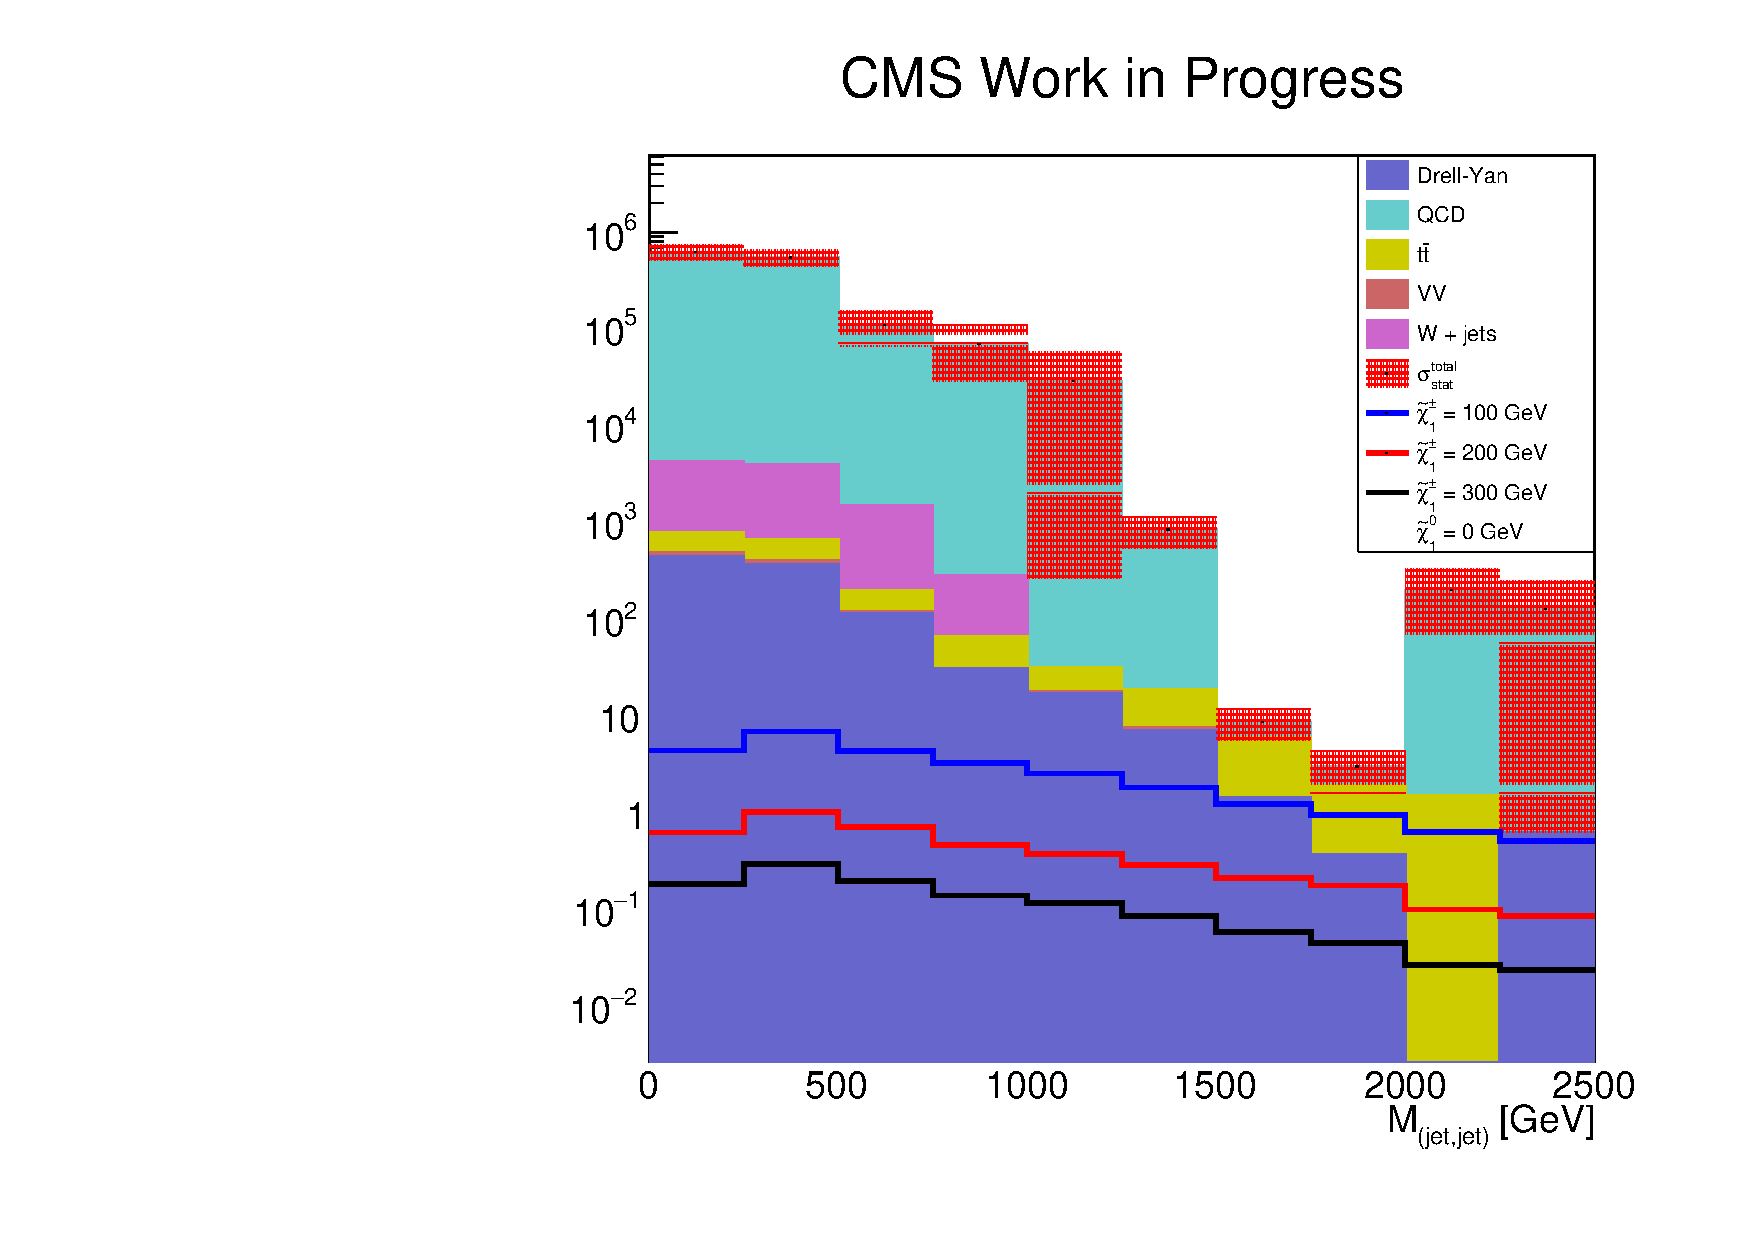
\includegraphics[width=0.5\textwidth]{analysis/pics/h_dijetinvariantmass_Taui2TightIso.pdf}
		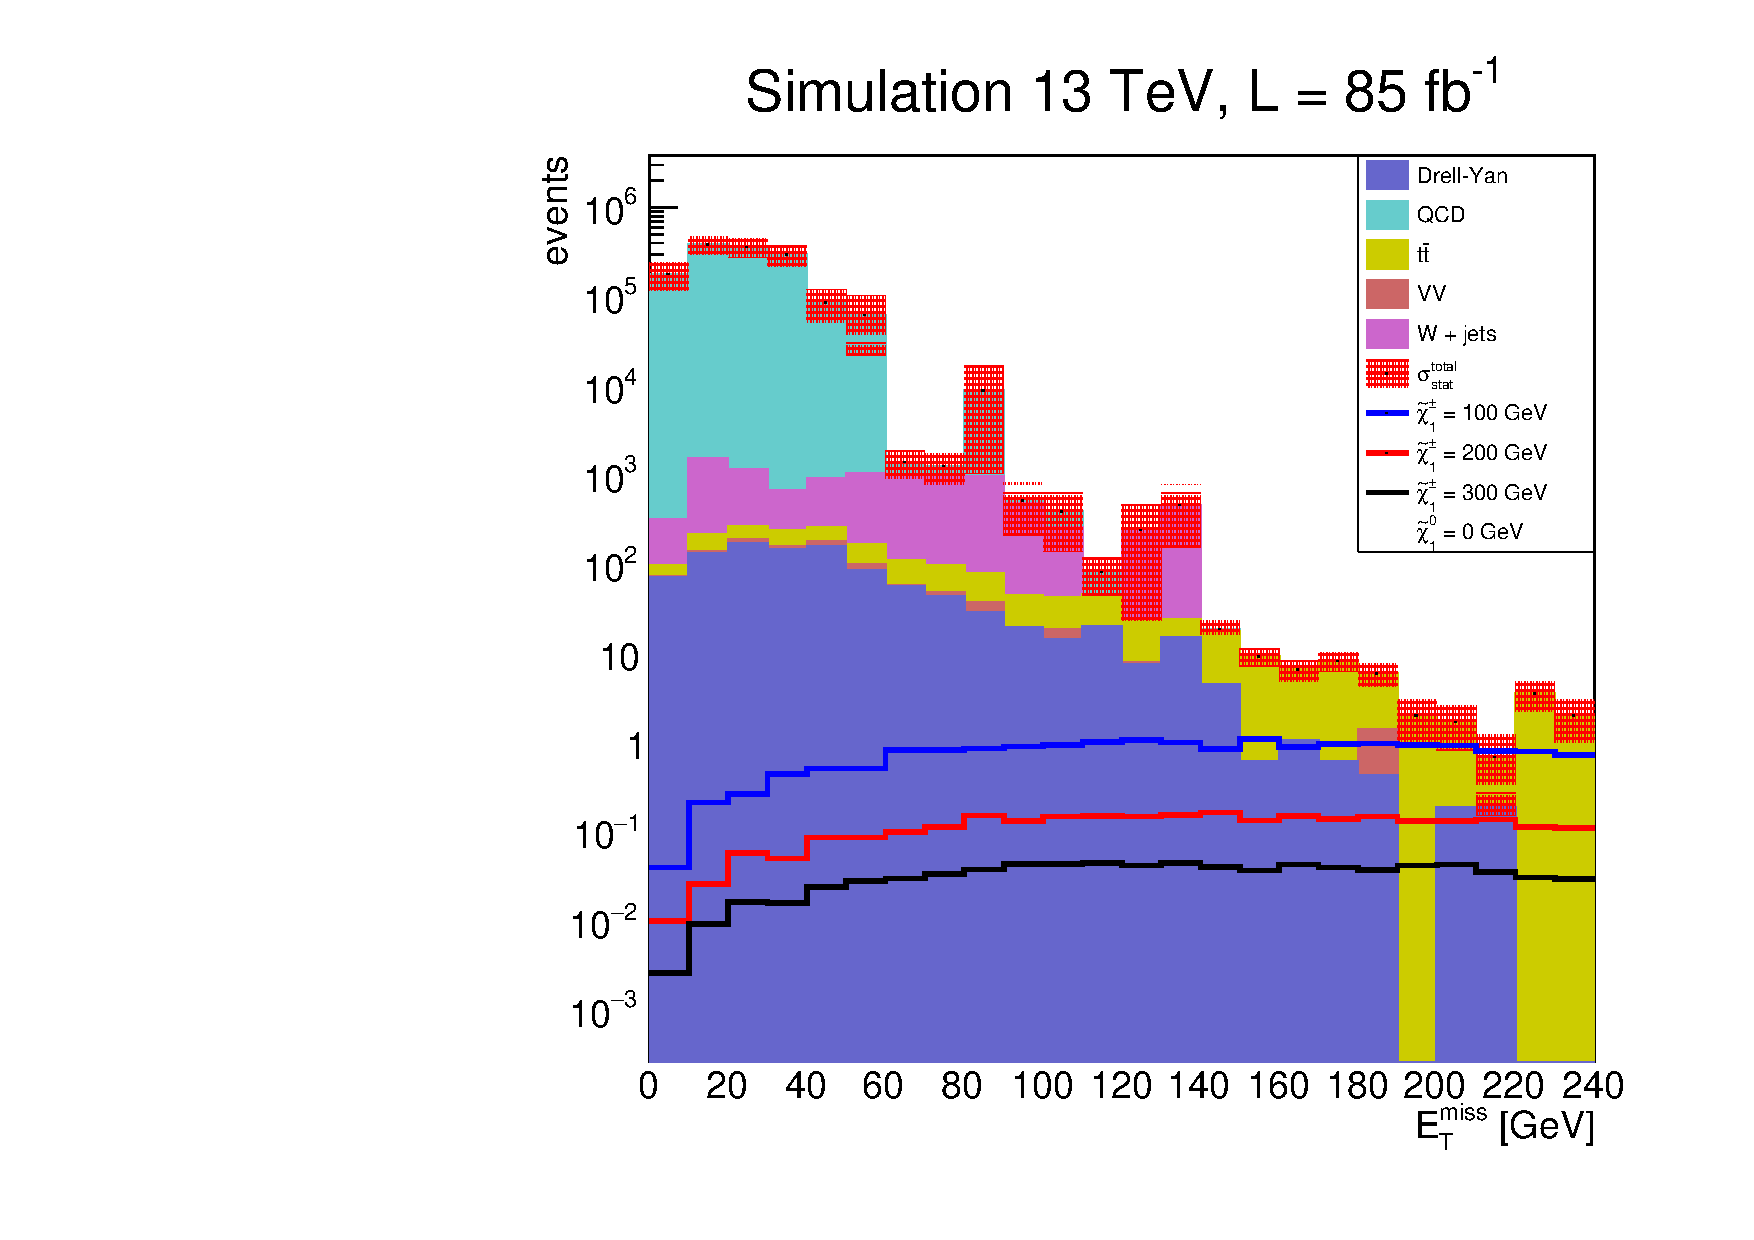
\includegraphics[width=0.5\textwidth]{analysis/pics/h_met_Taui2TightIso.pdf}
	\end{tabular}
	\caption{(Left) Di-jet invariant mass distribution and (Right) and \met distribution of selected signal and all MC background samples in signal region.}
	\label{fig::crplots1_Taui2TightIso_13tev}
\end{figure}

\begin{figure}[tbh!]
	\centering
	\begin{tabular}{cc}
		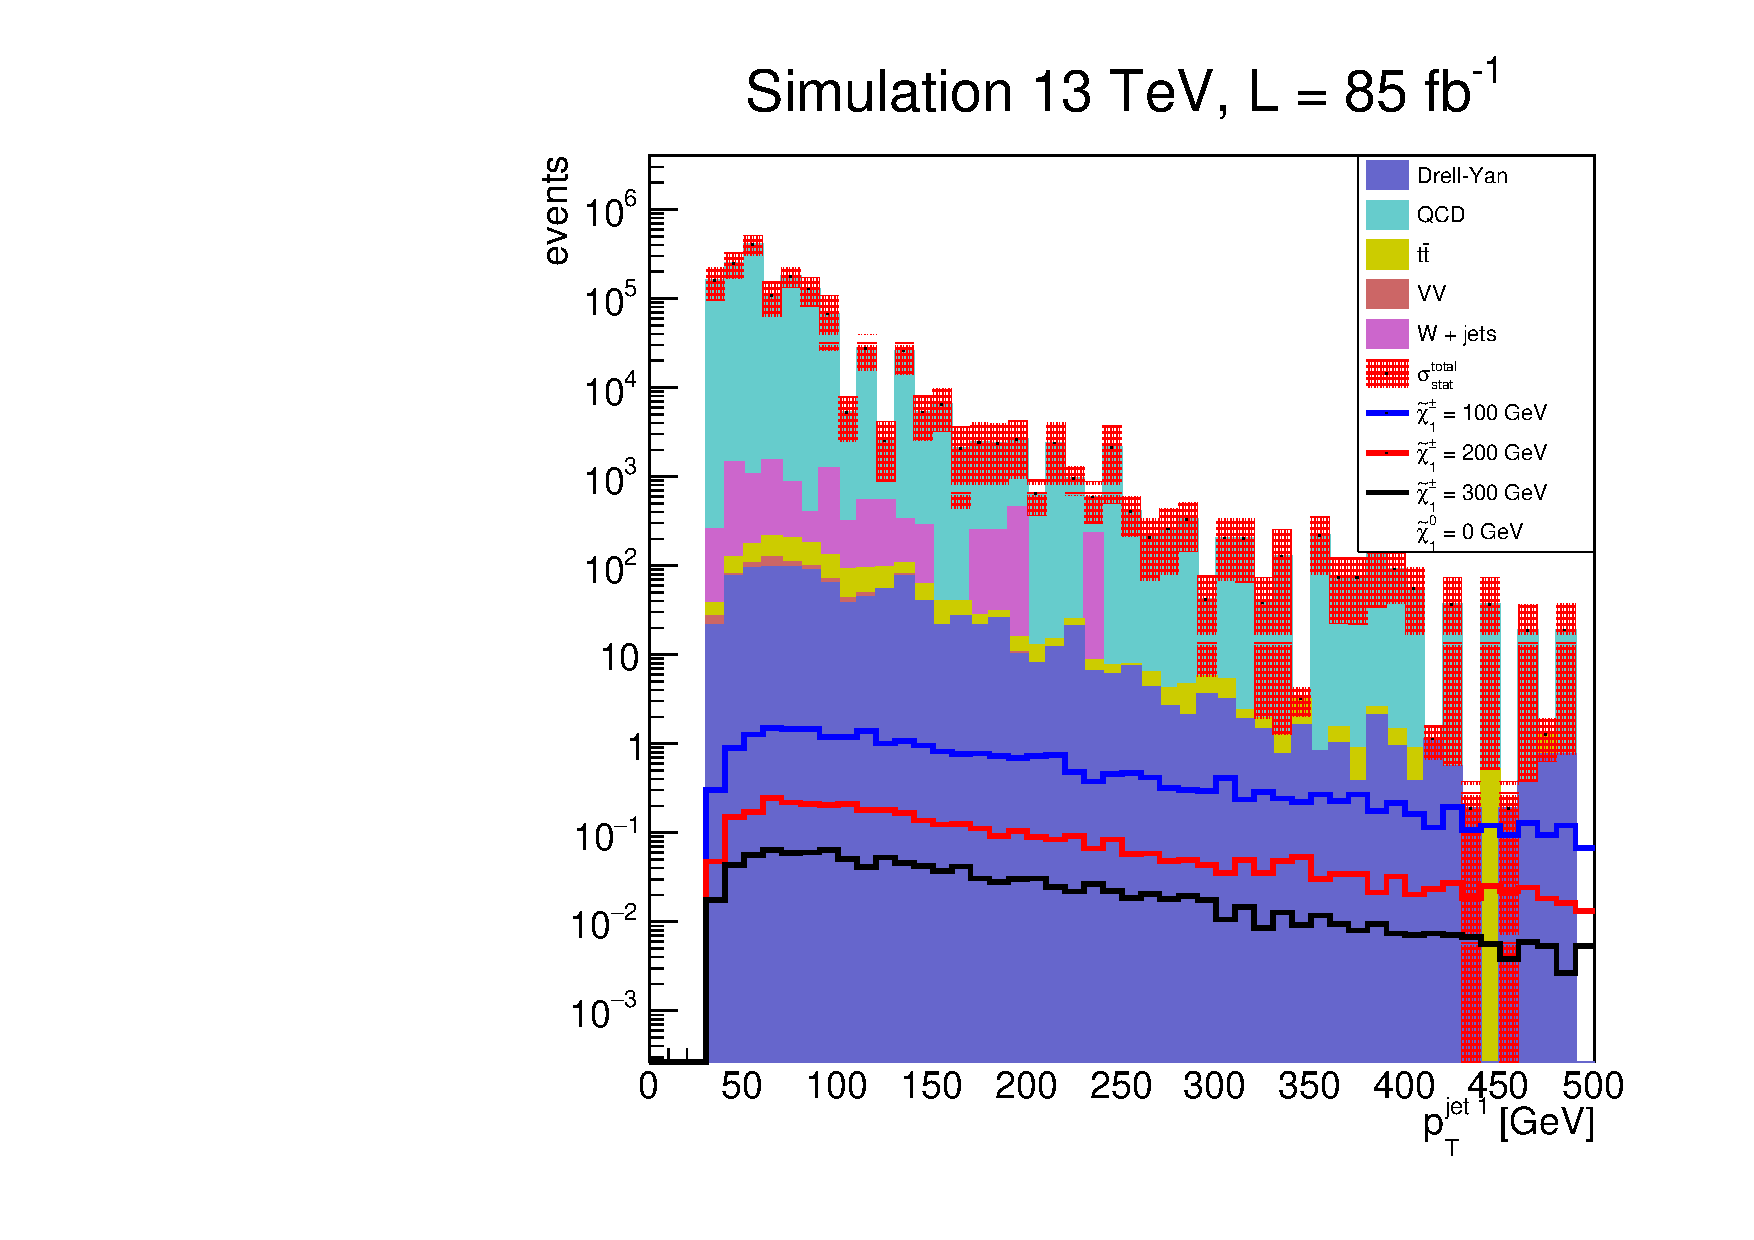
\includegraphics[width=0.5\textwidth]{analysis/pics/h_jet1pt_Taui2TightIso.pdf}
		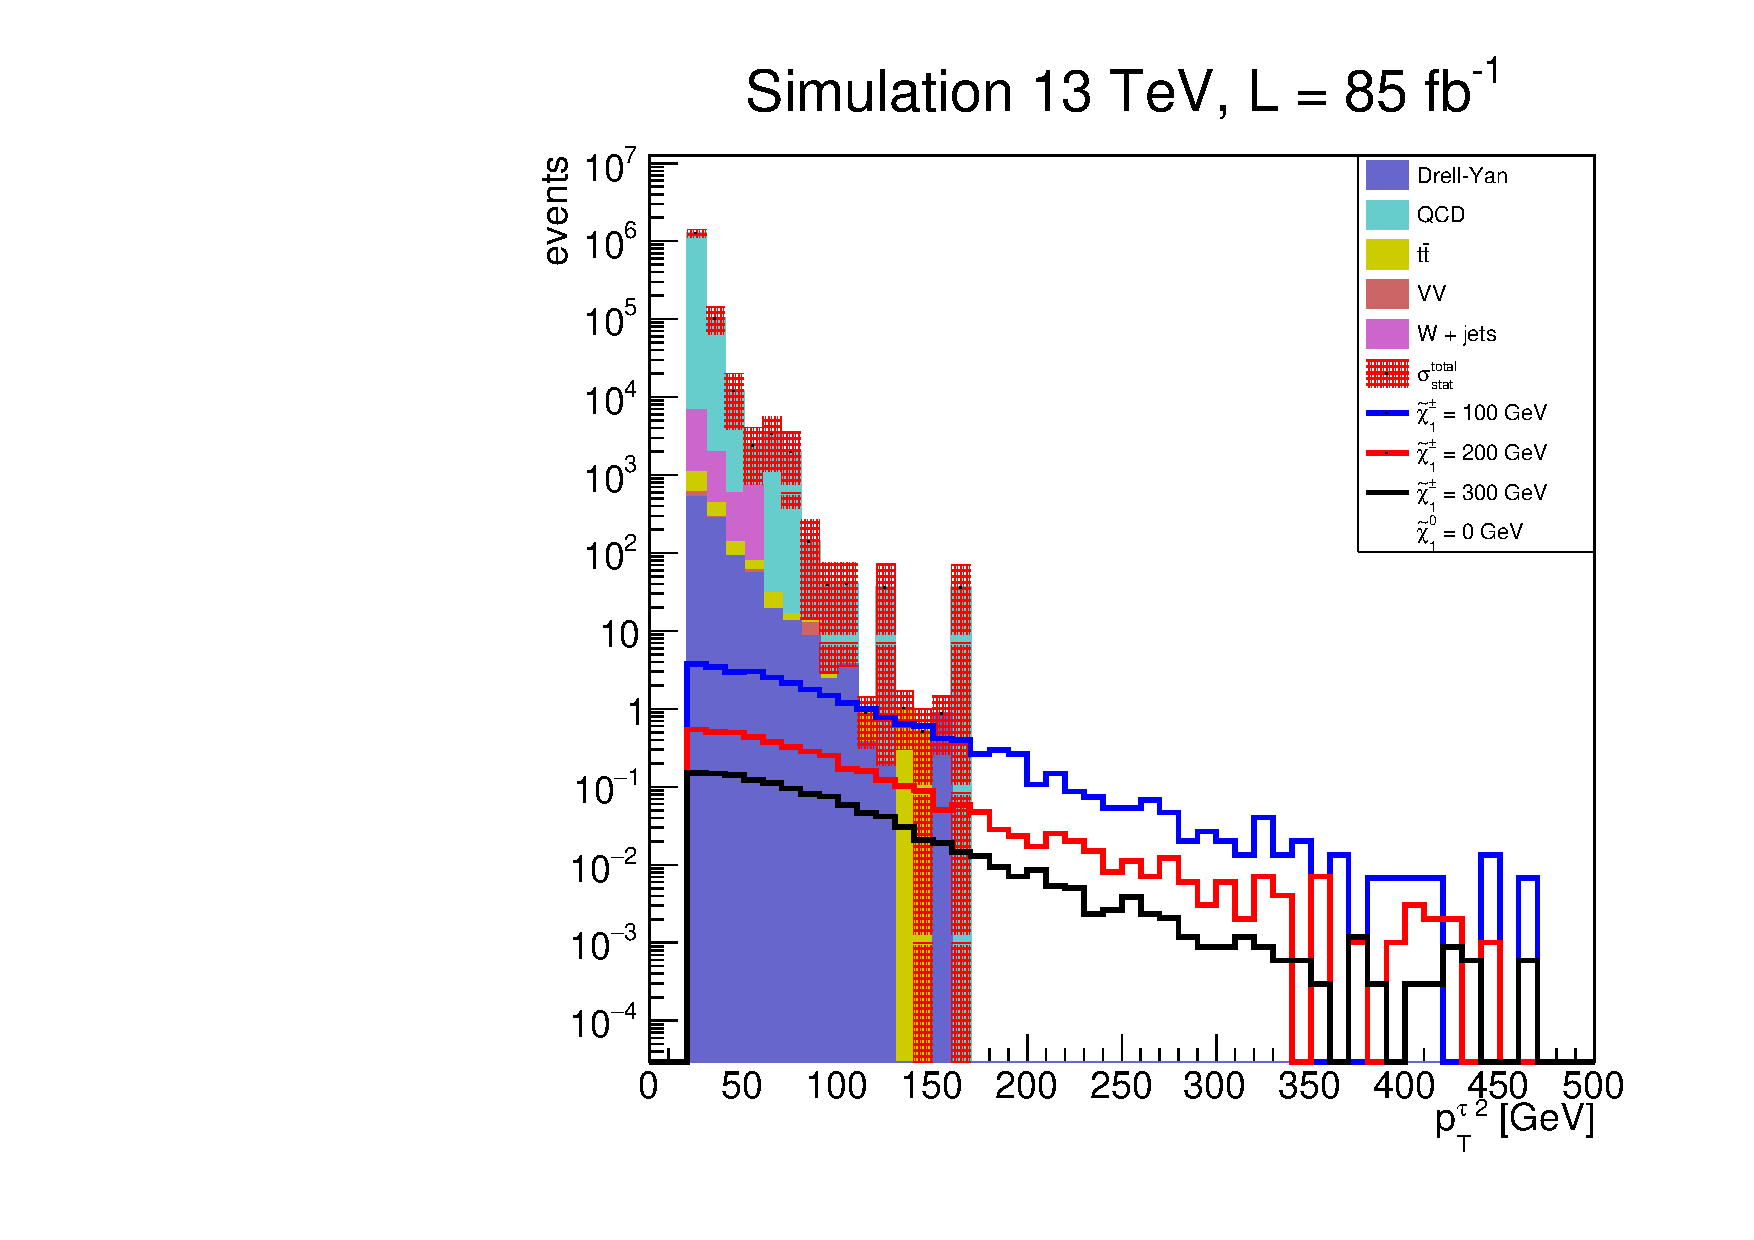
\includegraphics[width=0.5\textwidth]{analysis/pics/h_tau2pt_Taui2TightIso.pdf}
	\end{tabular}
	\caption{(Left) Leading jet \pt distribution and (Right) and second leading \hadtau \pt distribution of selected signal and all MC background samples in signal region.}
	\label{fig::crplots2_Taui2TightIso_13tev}
\end{figure}

\subsection*{Control region 2}

\FloatBarrier

2 tight-isolated \hadtau, inverted VBF selection

\begin{figure}[tbh!]
	\centering
	\begin{tabular}{cc}
		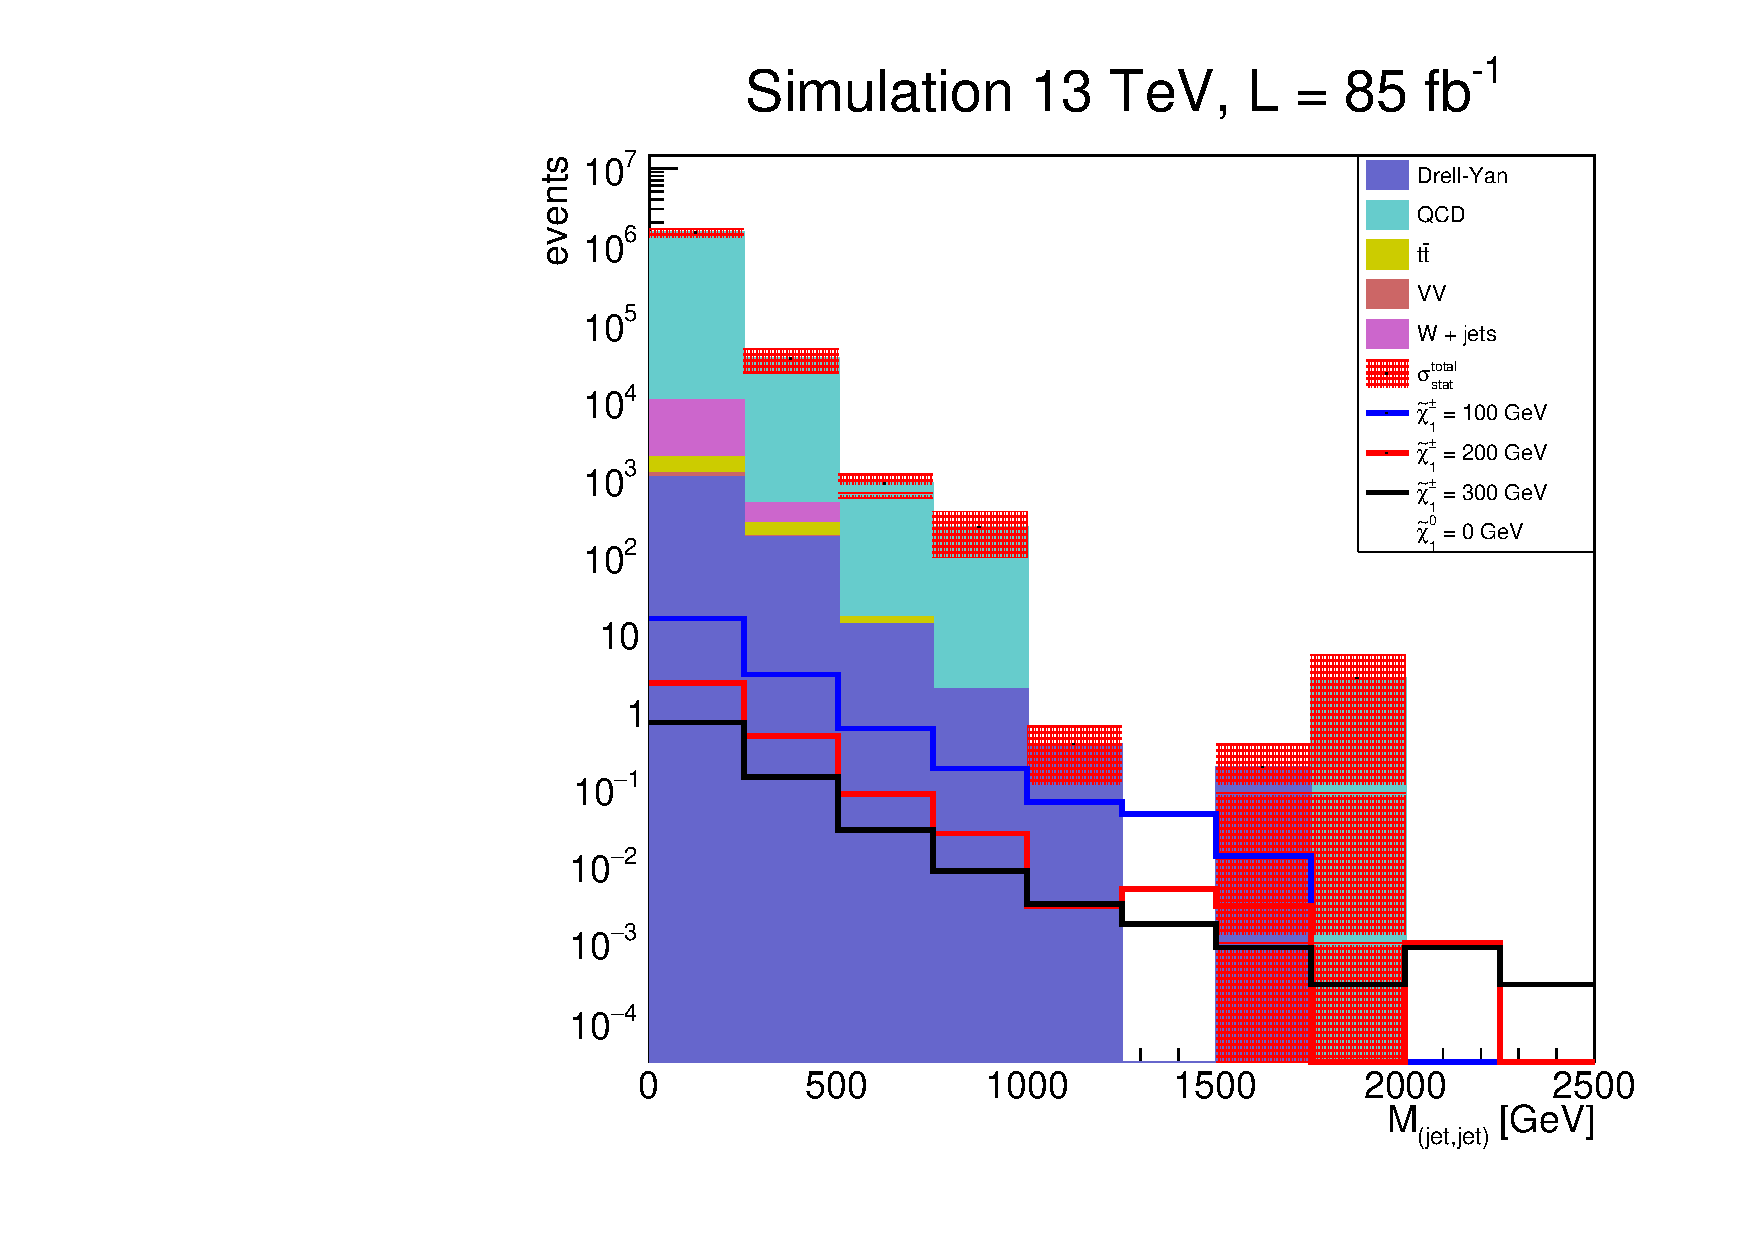
\includegraphics[width=0.5\textwidth]{analysis/pics/h_dijetinvariantmass_Tau2TightIsoVBFInverted.pdf}
		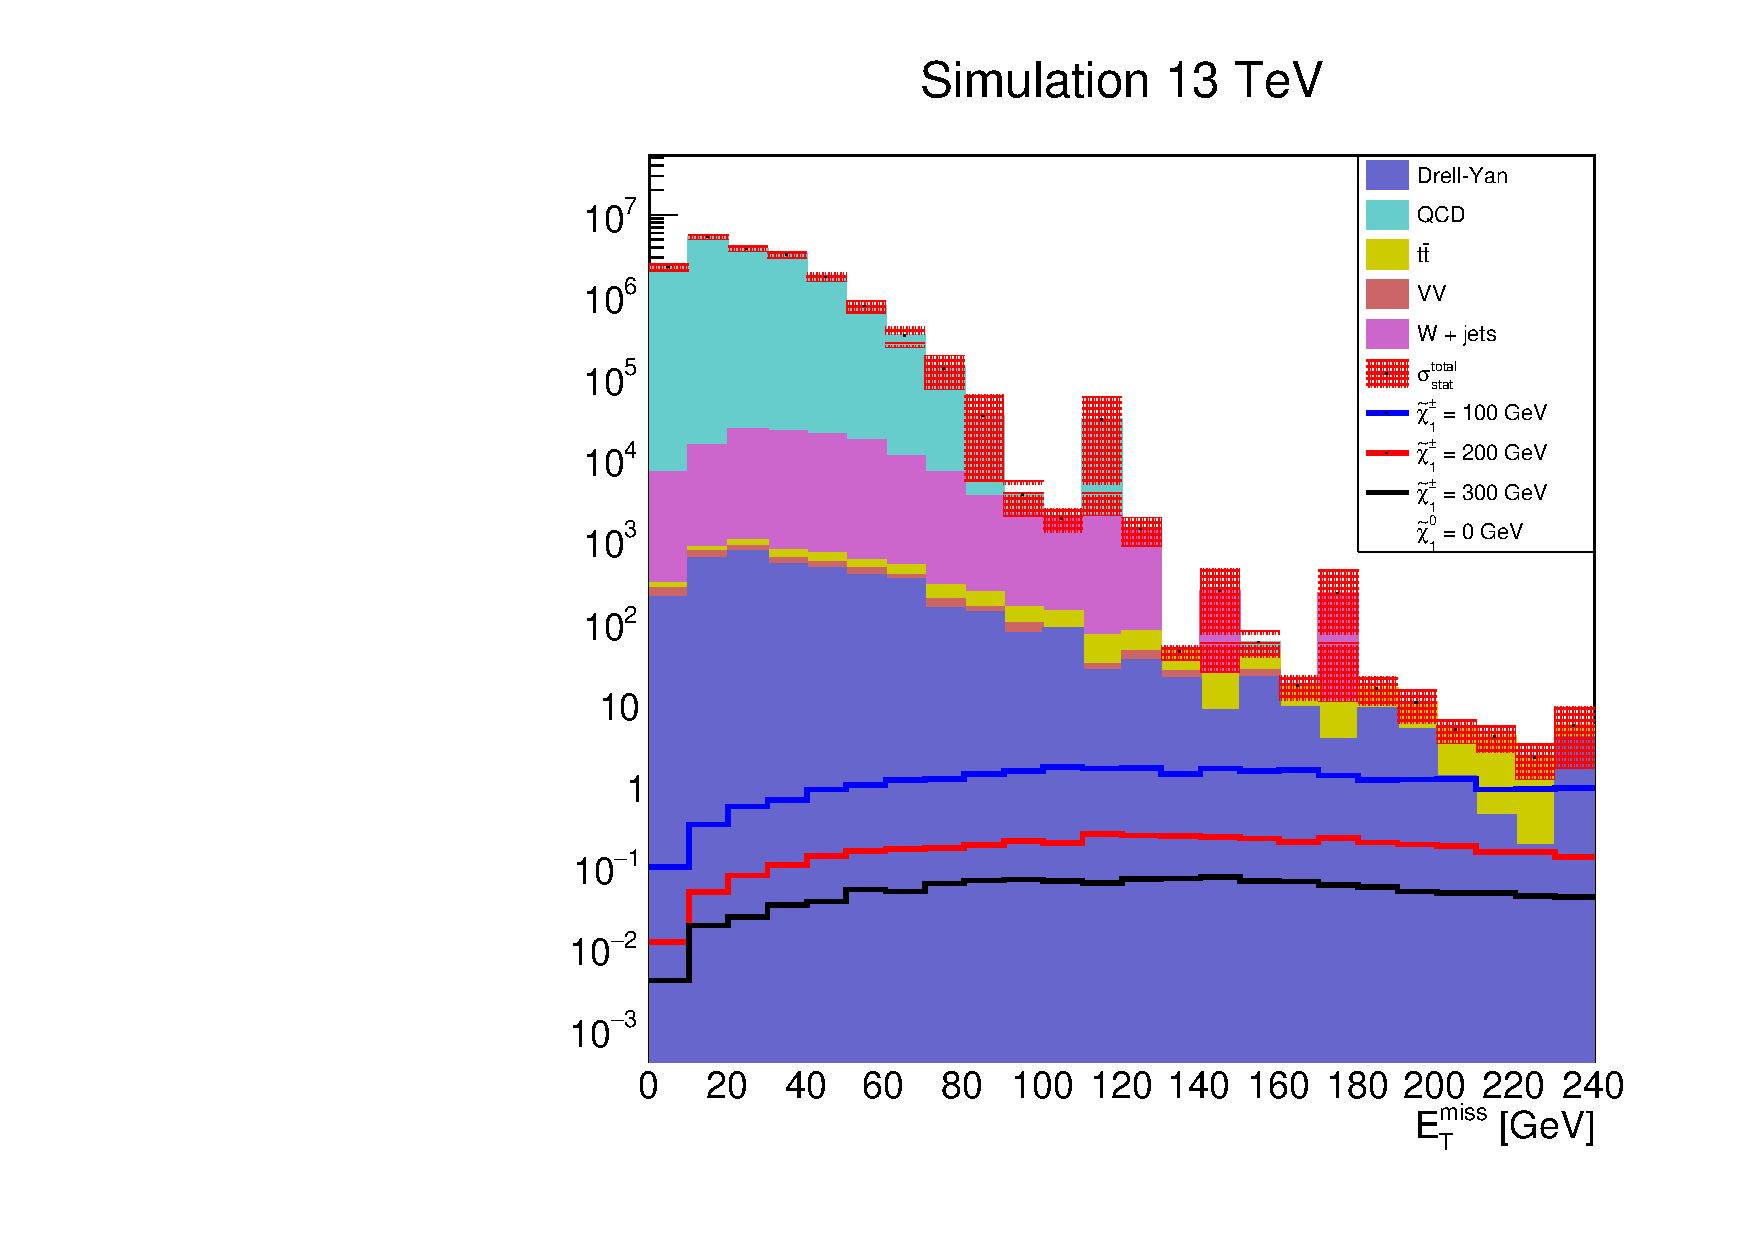
\includegraphics[width=0.5\textwidth]{analysis/pics/h_met_Tau2TightIsoVBFInverted.pdf}
	\end{tabular}
	\caption{(Left) Di-jet invariant mass distribution and (Right) and \met distribution of selected signal and all MC background samples in control region 2.}
	\label{fig::crplots1_Tau2TightIsoVBFInverted_13tev}
\end{figure}

\begin{figure}[tbh!]
	\centering
	\begin{tabular}{cc}
		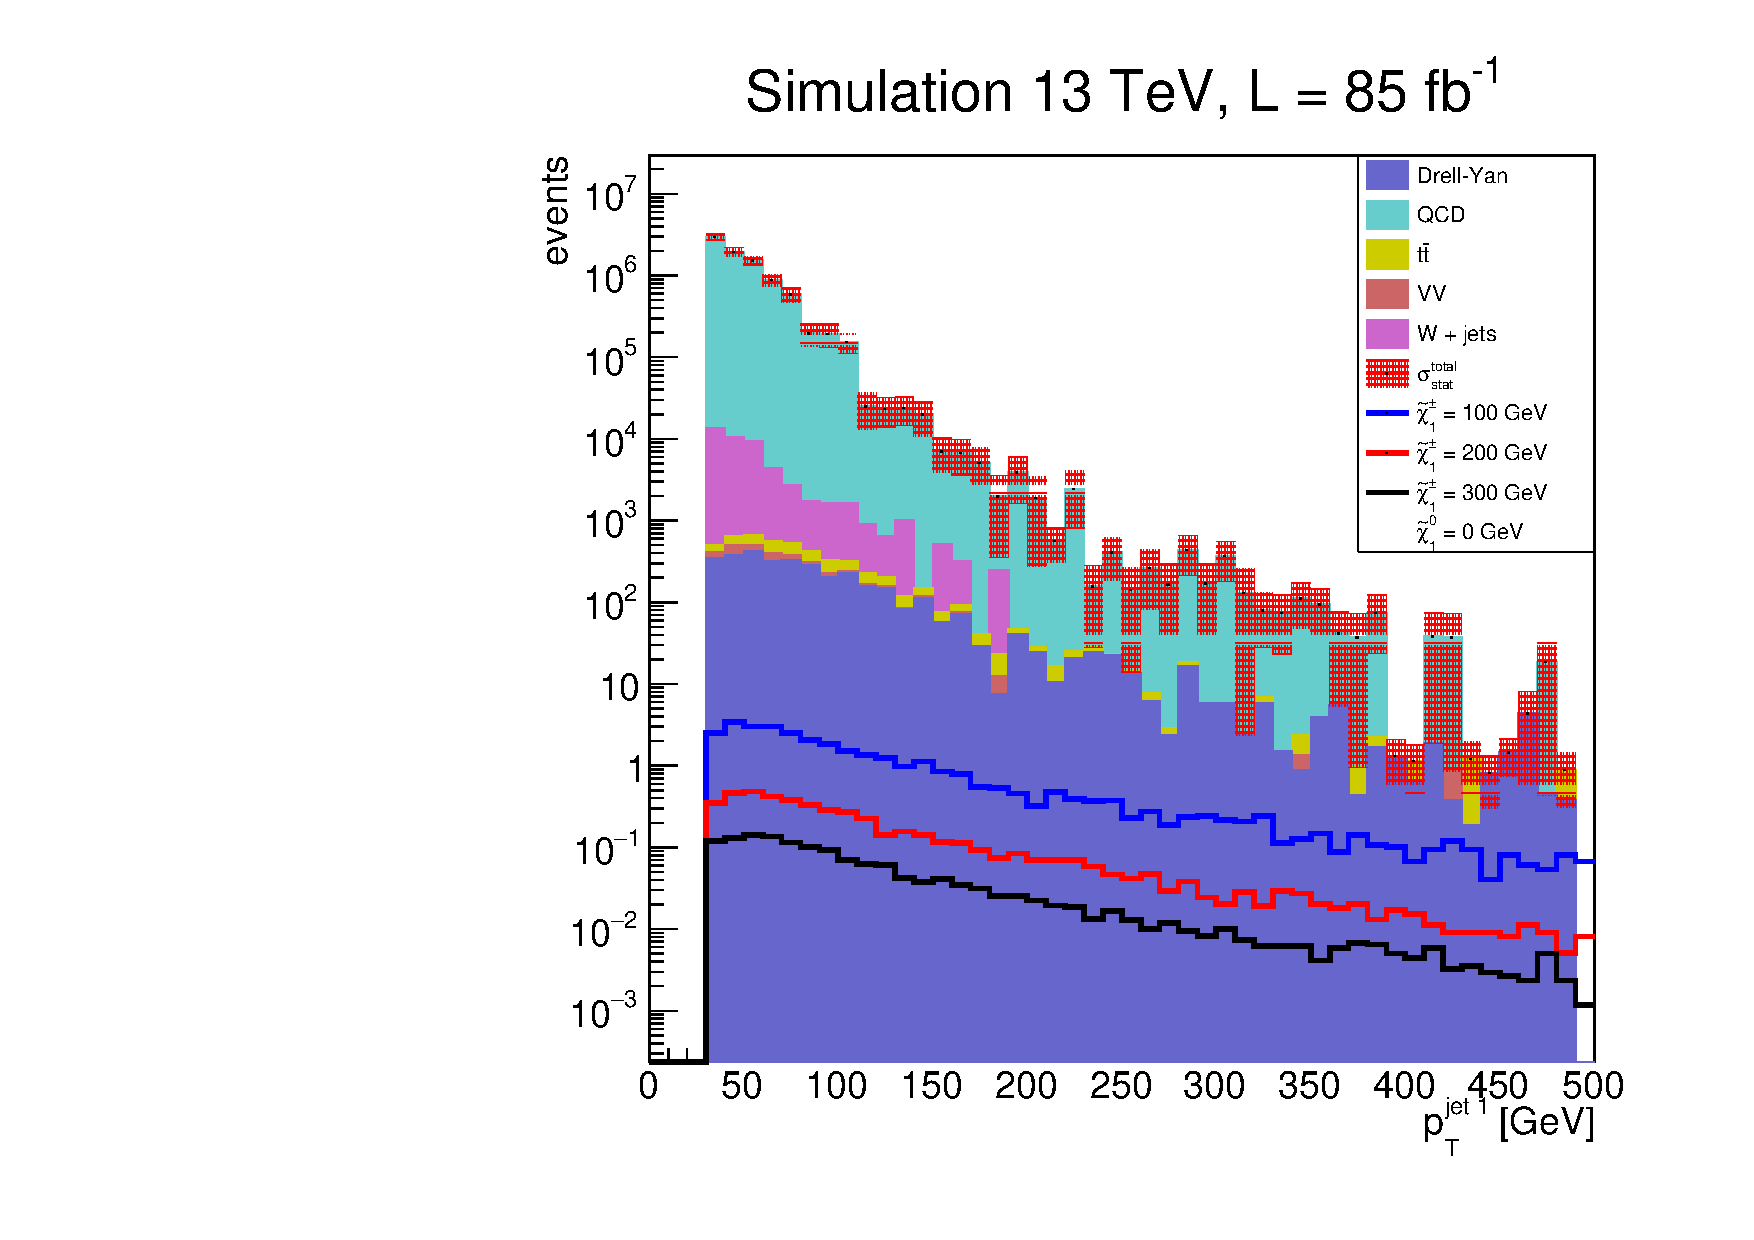
\includegraphics[width=0.5\textwidth]{analysis/pics/h_jet1pt_Tau2TightIsoVBFInverted.pdf}
		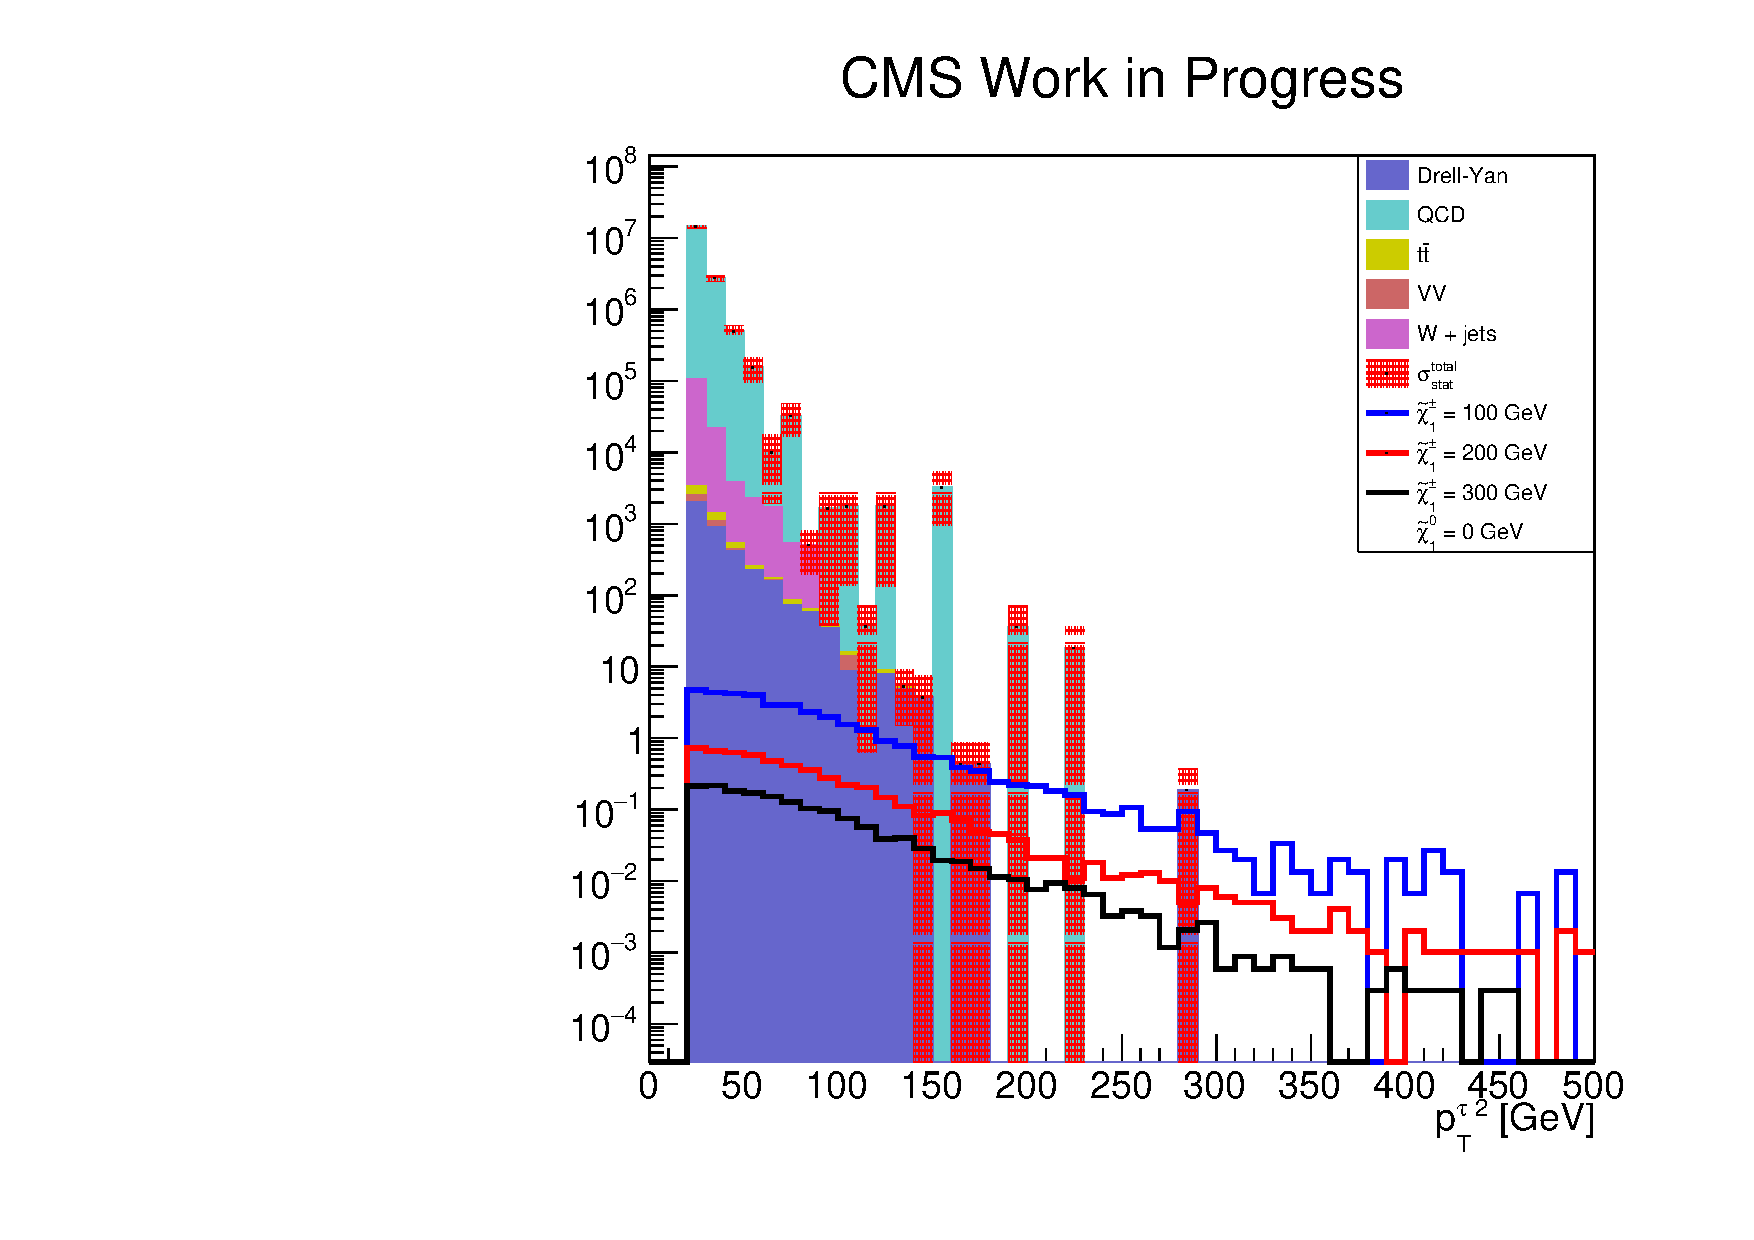
\includegraphics[width=0.5\textwidth]{analysis/pics/h_tau2pt_Tau2TightIsoVBFInverted.pdf}
	\end{tabular}
	\caption{(Left) Leading jet \pt distribution and (Right) and second leading \hadtau \pt distribution of selected signal and all MC background samples in control region 2.}
	\label{fig::crplots2_Taui2TightIsoVBFInverted_13tev}
\end{figure}

\subsection*{Control region 3}

\FloatBarrier

2 loose-isolated \hadtau (inclusive)

\begin{figure}[tbh!]
	\centering
	\begin{tabular}{cc}
		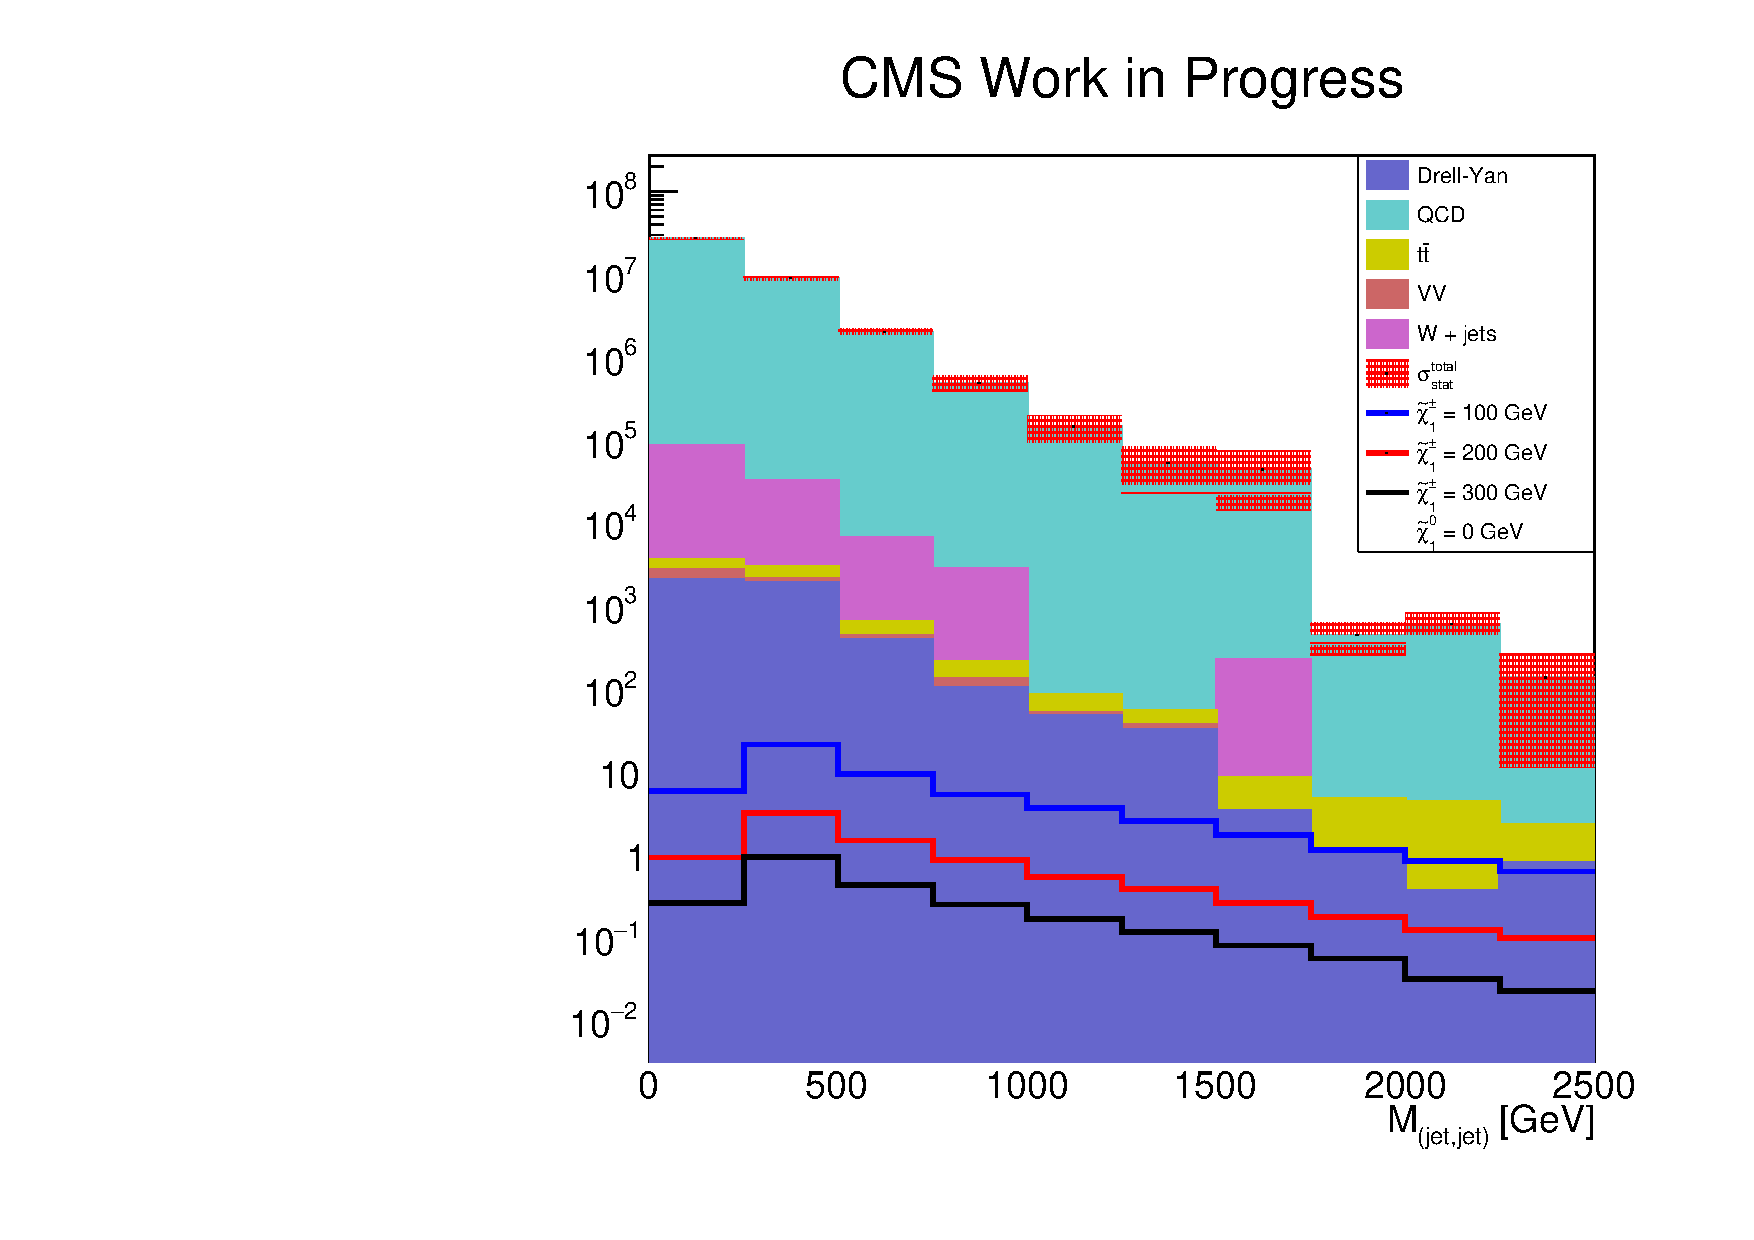
\includegraphics[width=0.5\textwidth]{analysis/pics/h_dijetinvariantmass_Tau2LooseIsoInclusive.pdf}
		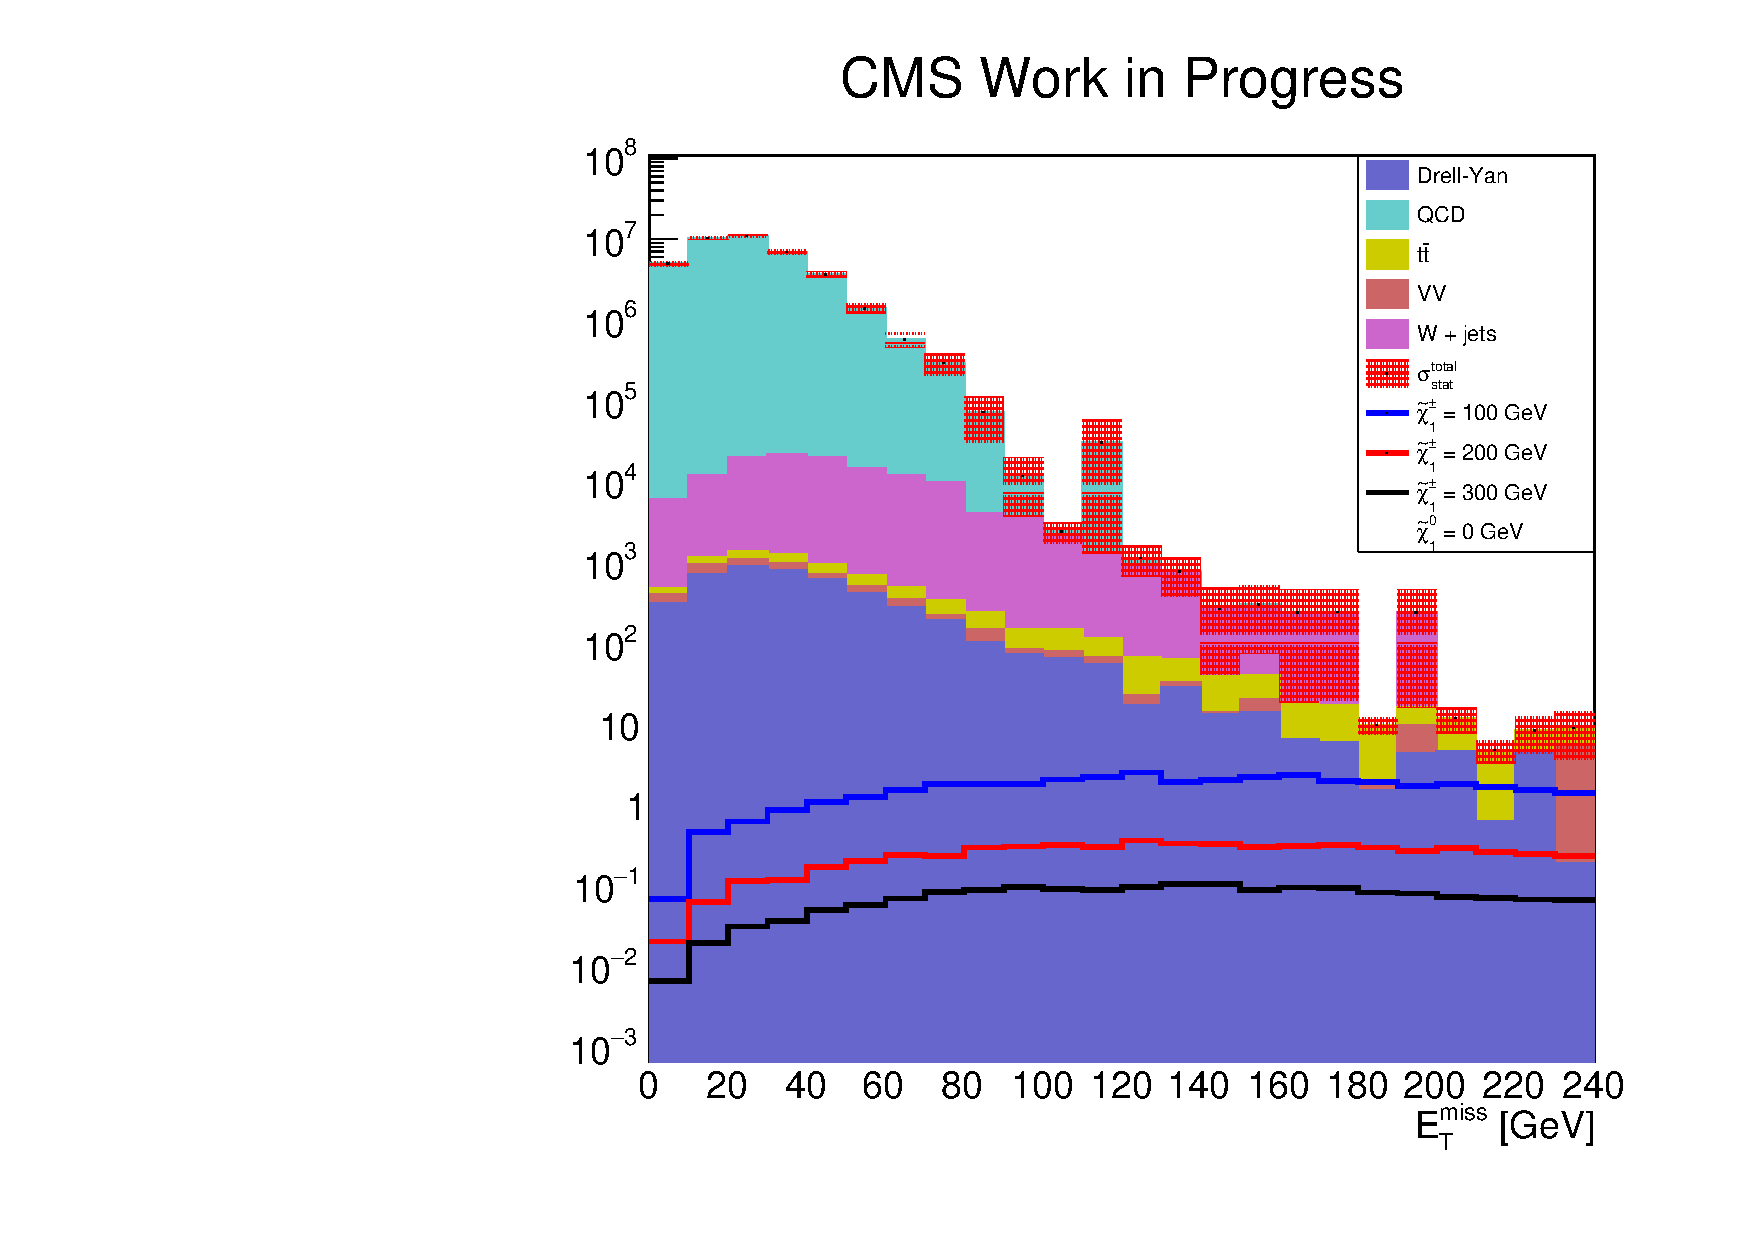
\includegraphics[width=0.5\textwidth]{analysis/pics/h_met_Tau2LooseIsoInclusive.pdf}
	\end{tabular}
	\caption{(Left) Di-jet invariant mass distribution and (Right) and \met distribution of selected signal and all MC background samples in control region 3.}
	\label{fig::crplots1_Tau2LooseIsoInclusive_13tev}
\end{figure}

\begin{figure}[tbh!]
	\centering
	\begin{tabular}{cc}
		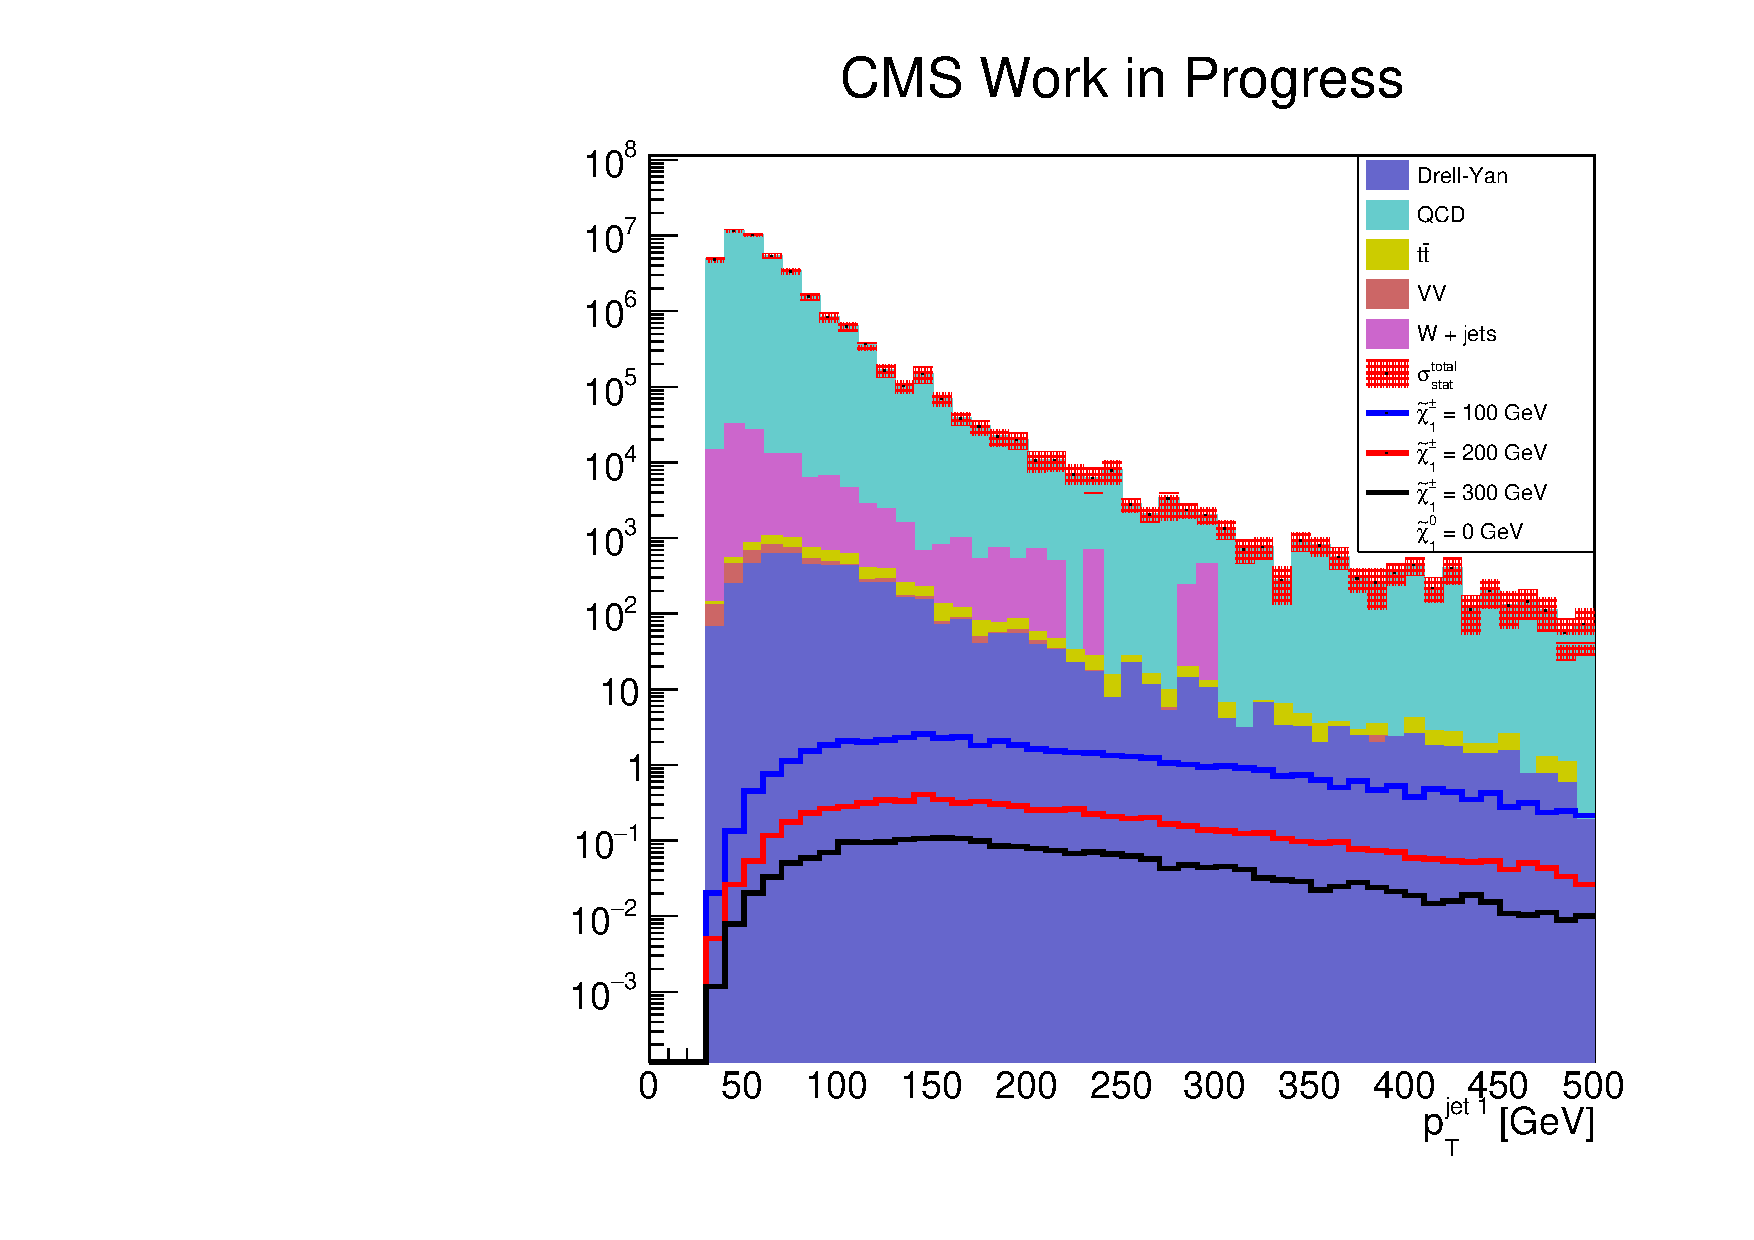
\includegraphics[width=0.5\textwidth]{analysis/pics/h_jet1pt_Tau2LooseIsoInclusive.pdf}
		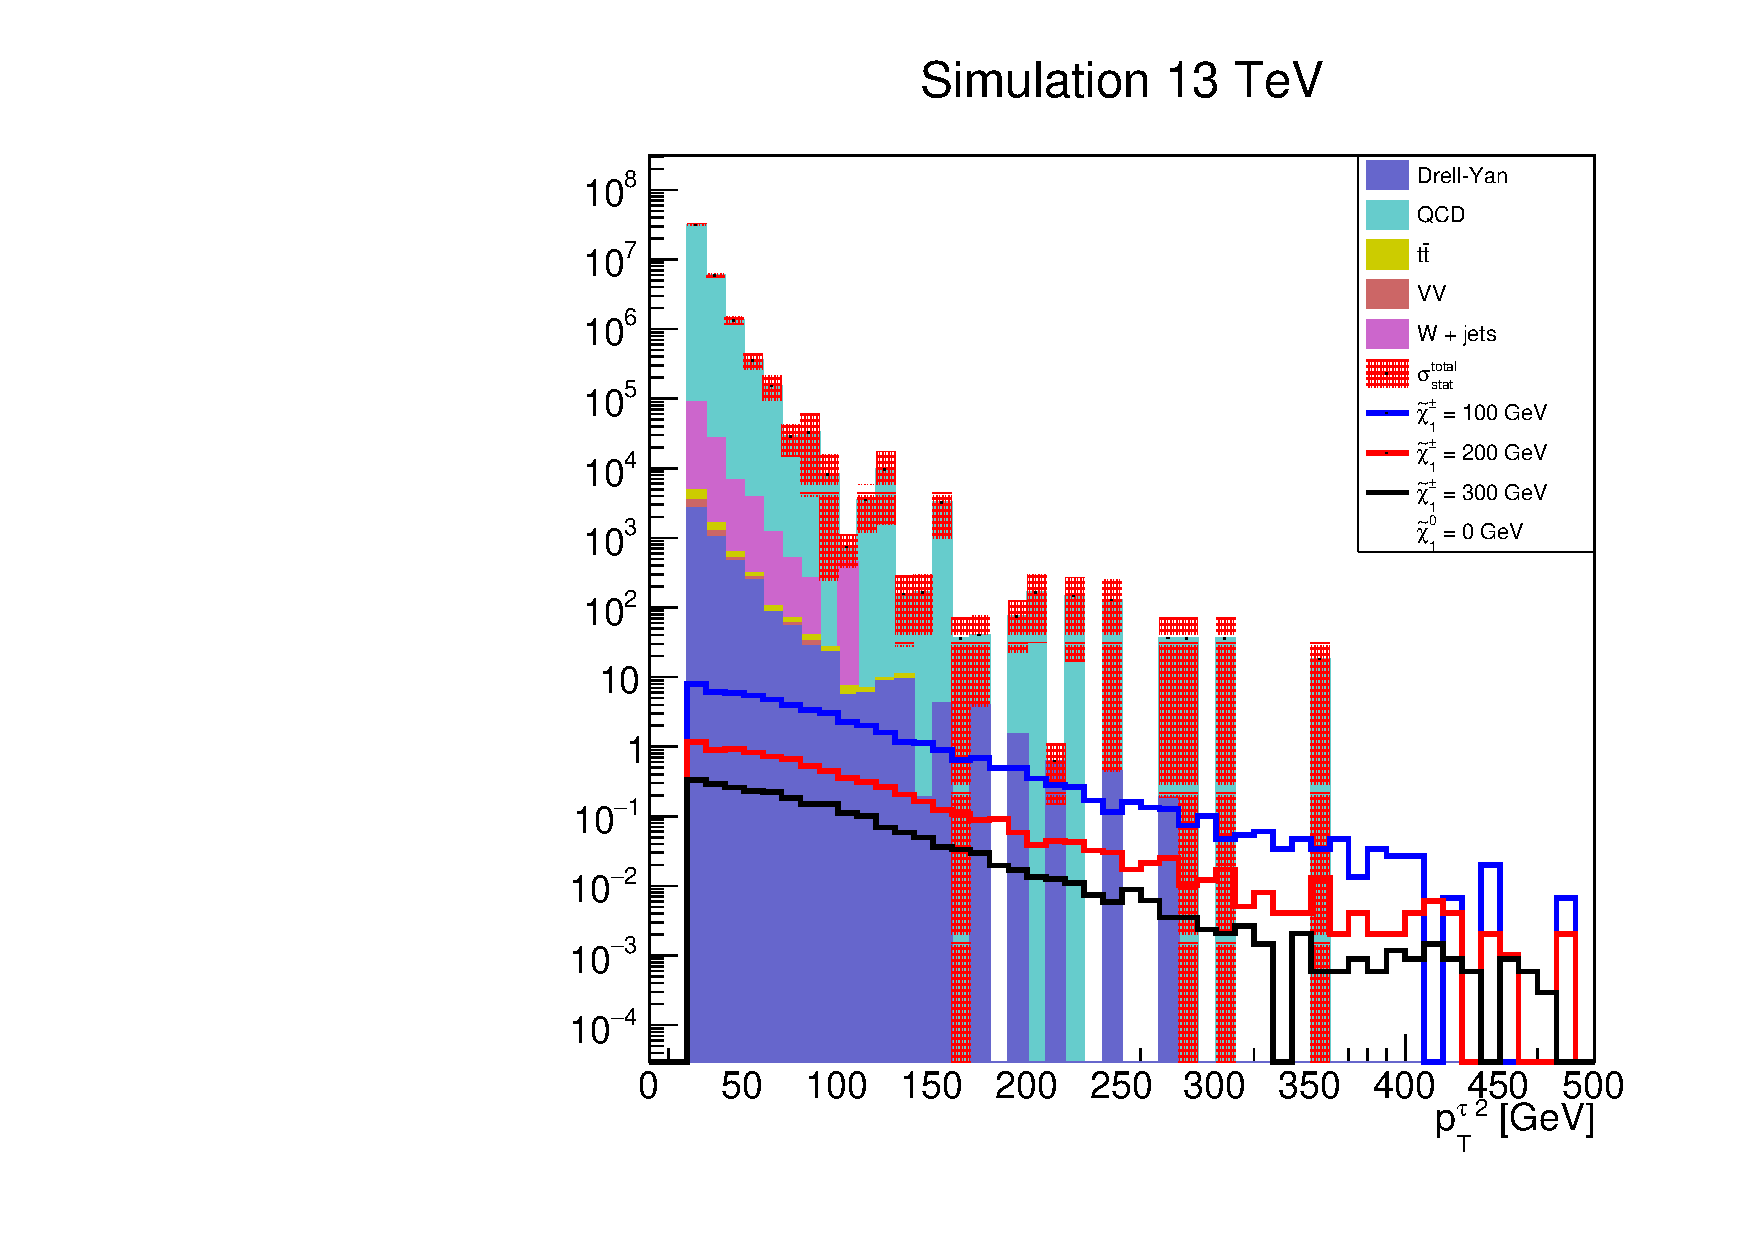
\includegraphics[width=0.5\textwidth]{analysis/pics/h_tau2pt_Tau2LooseIsoInclusive.pdf}
	\end{tabular}
	\caption{(Left) Leading jet \pt distribution and (Right) and second leading \hadtau \pt distribution of selected signal and all MC background samples in control region 3.}
	\label{fig::crplots2_Tau2LooseIsoInclusive_13tev}
\end{figure}

\subsection*{Control region 4}

\FloatBarrier

2 loose-isolated \hadtau (inclusive), inverted VBF selection

\begin{figure}[tbh!]
	\centering
	\begin{tabular}{cc}
		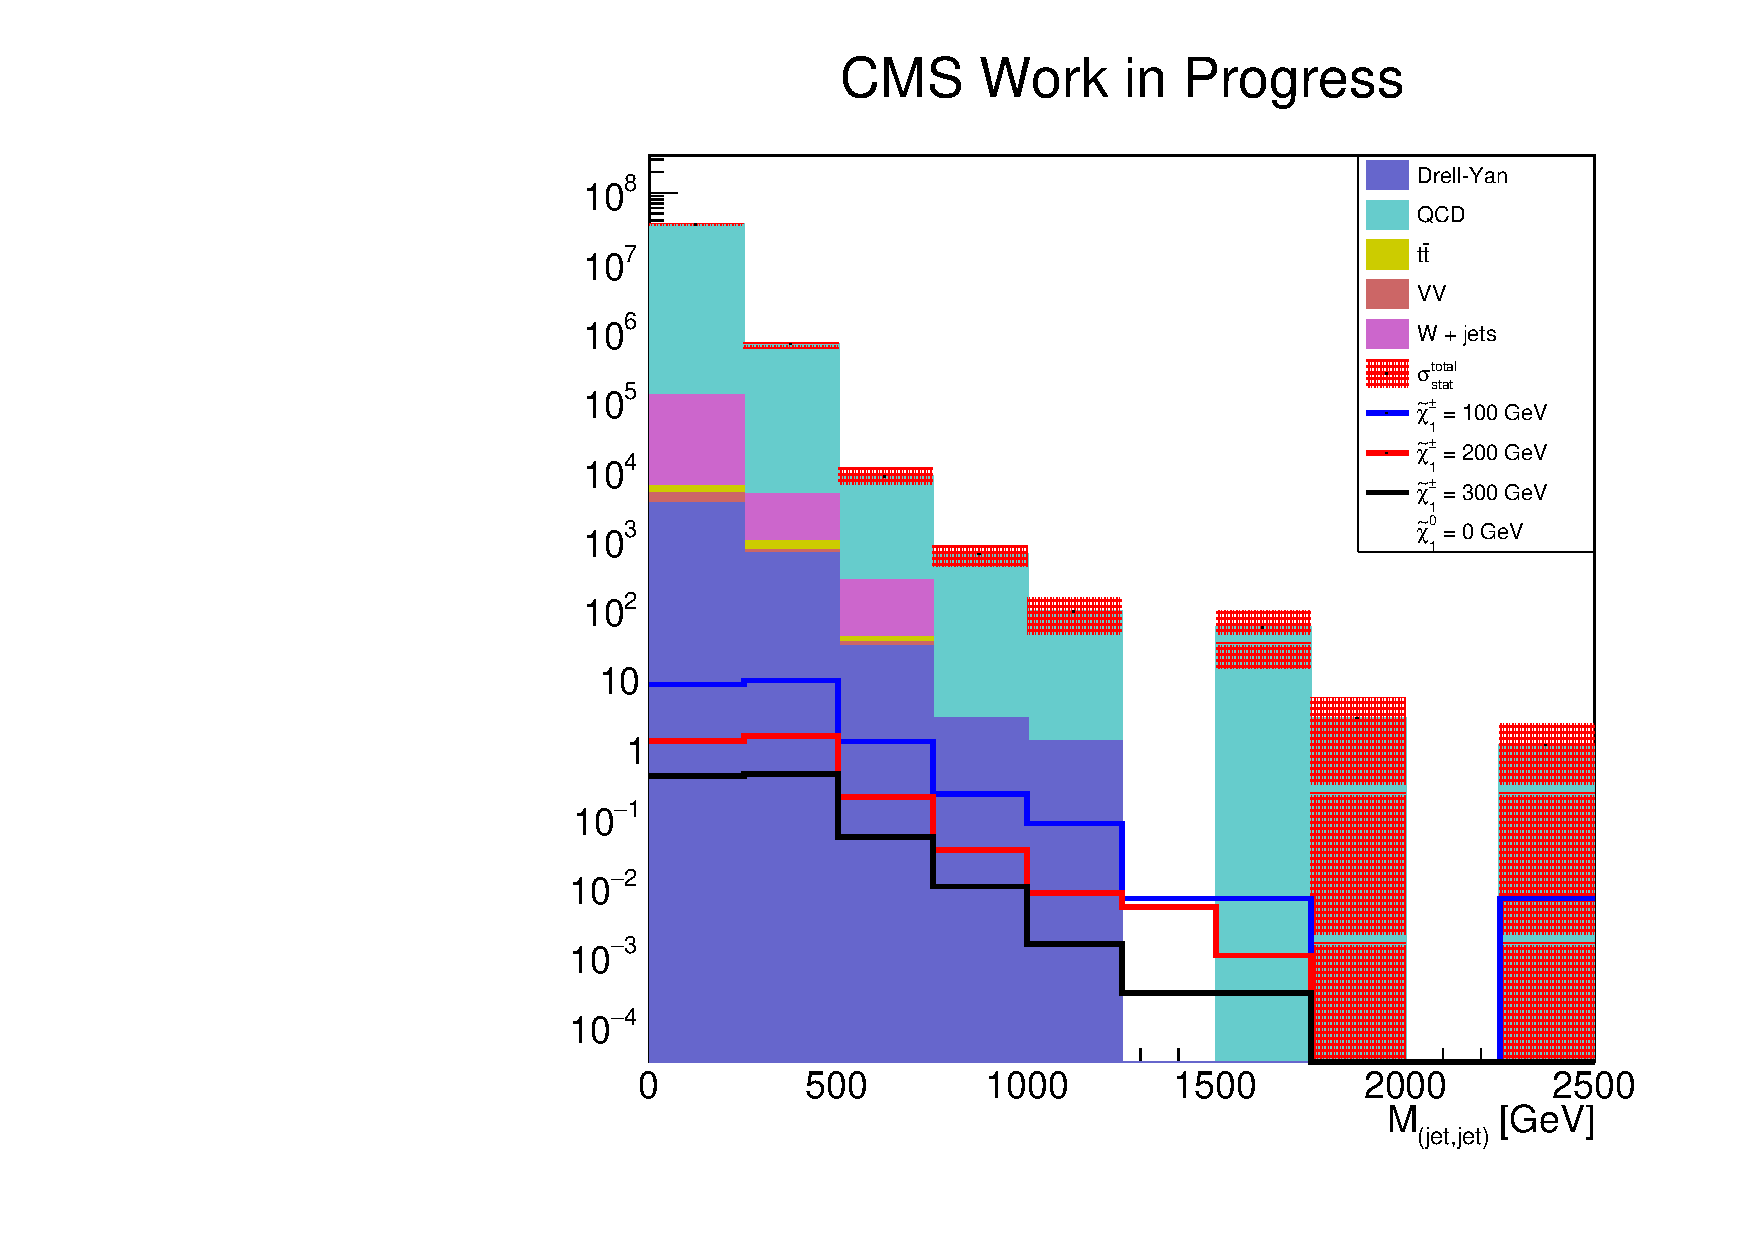
\includegraphics[width=0.5\textwidth]{analysis/pics/h_dijetinvariantmass_Tau2LooseIsoInclusiveVBFInverted.pdf}
		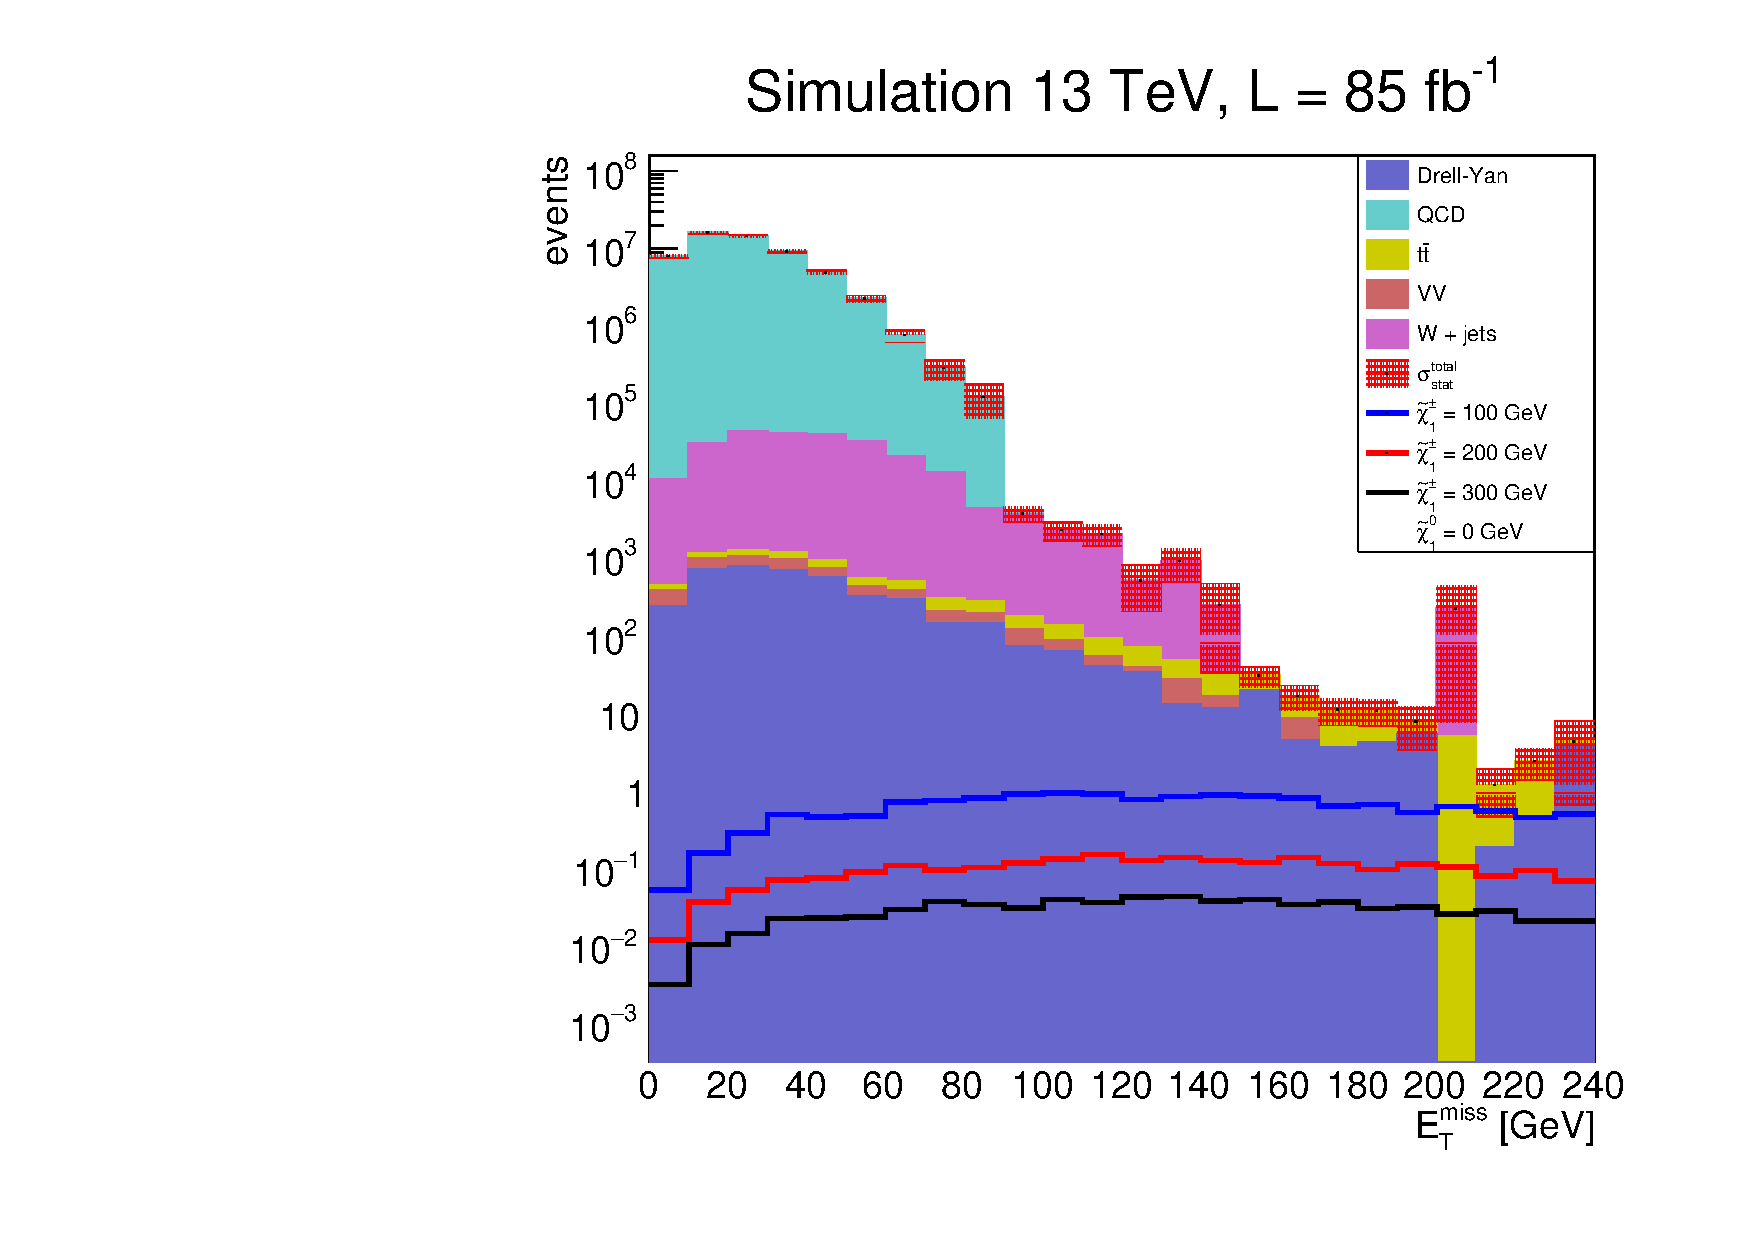
\includegraphics[width=0.5\textwidth]{analysis/pics/h_met_Tau2LooseIsoInclusiveVBFInverted.pdf}
	\end{tabular}
	\caption{(Left) Di-jet invariant mass distribution and (Right) and \met distribution of selected signal and all MC background samples in control region 4.}
	\label{fig::crplots1_Tau2LooseIsoInclusiveVBFInverted_13tev}
\end{figure}

\begin{figure}[tbh!]
	\centering
	\begin{tabular}{cc}
		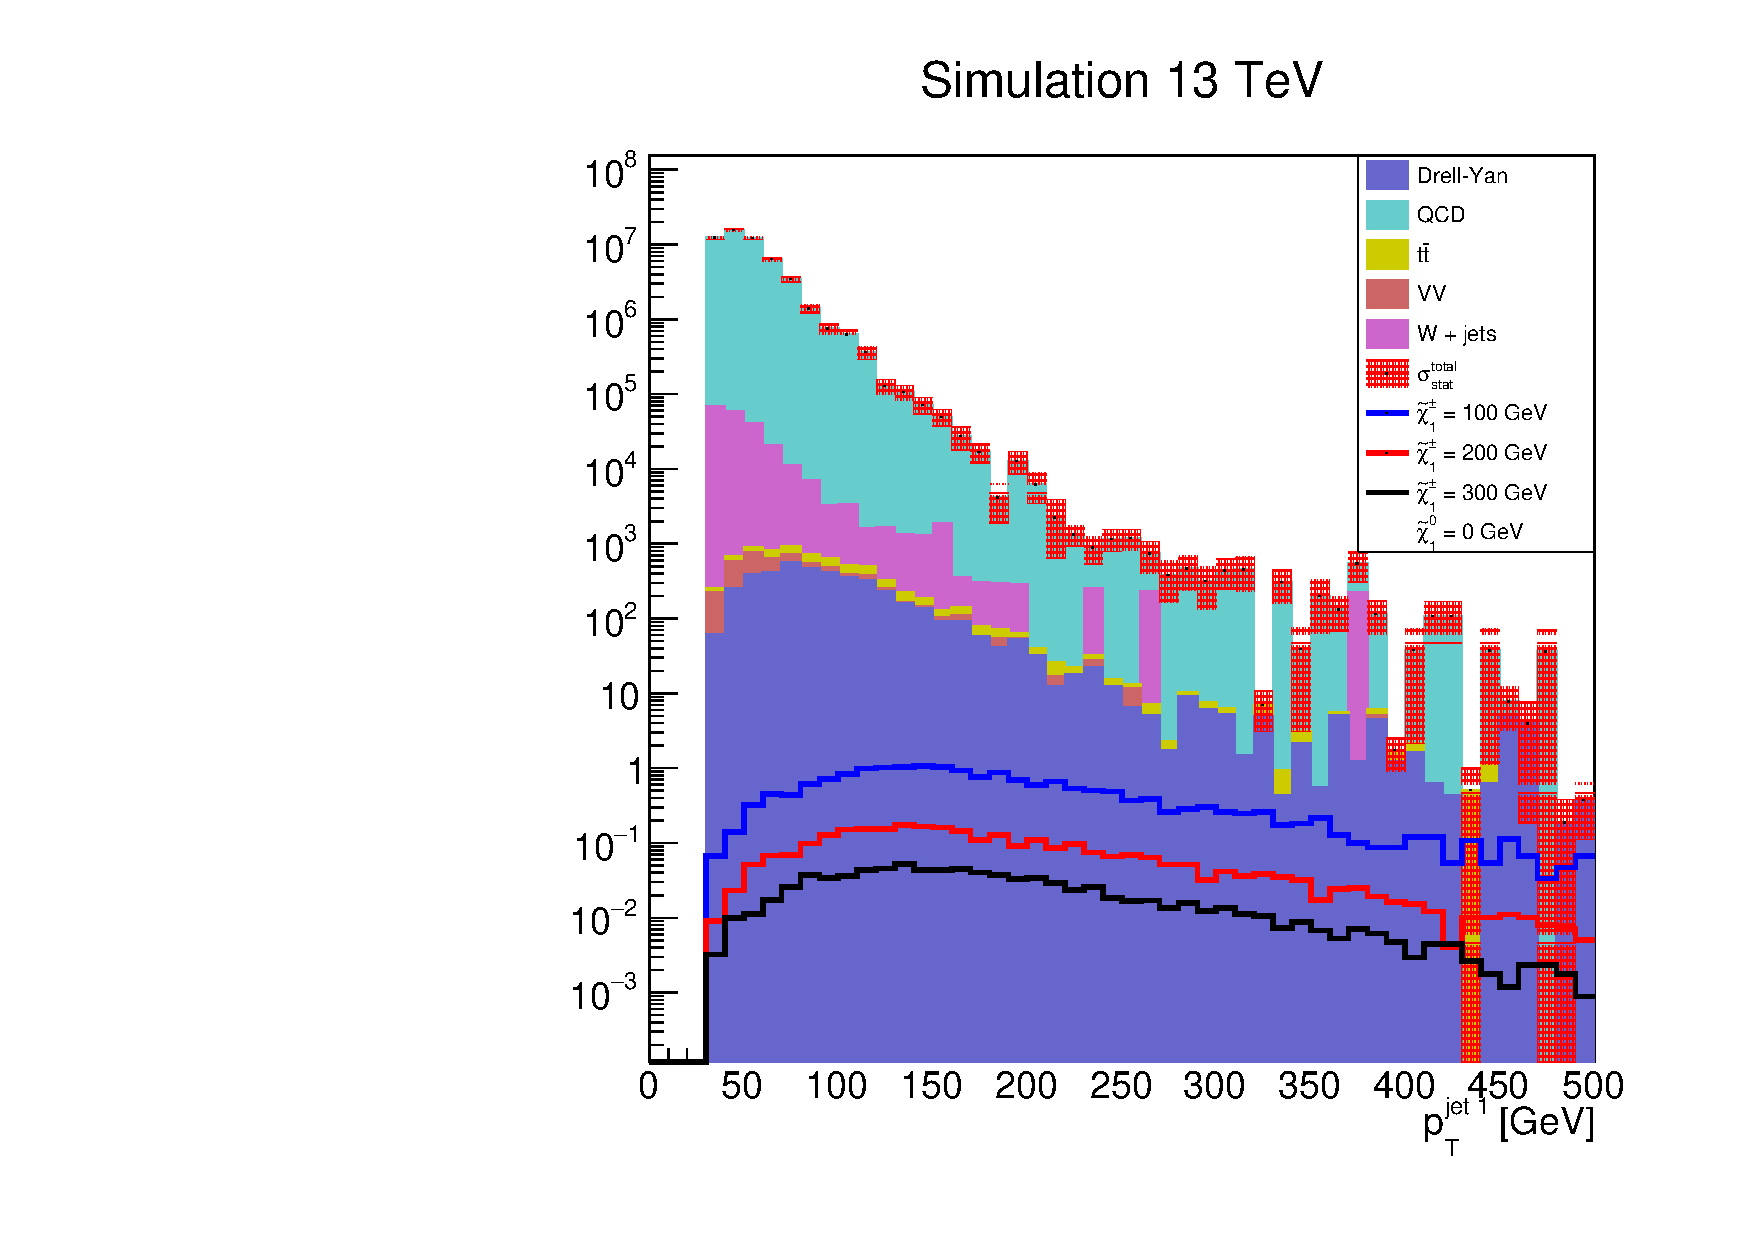
\includegraphics[width=0.5\textwidth]{analysis/pics/h_jet1pt_Tau2LooseIsoInclusiveVBFInverted.pdf}
		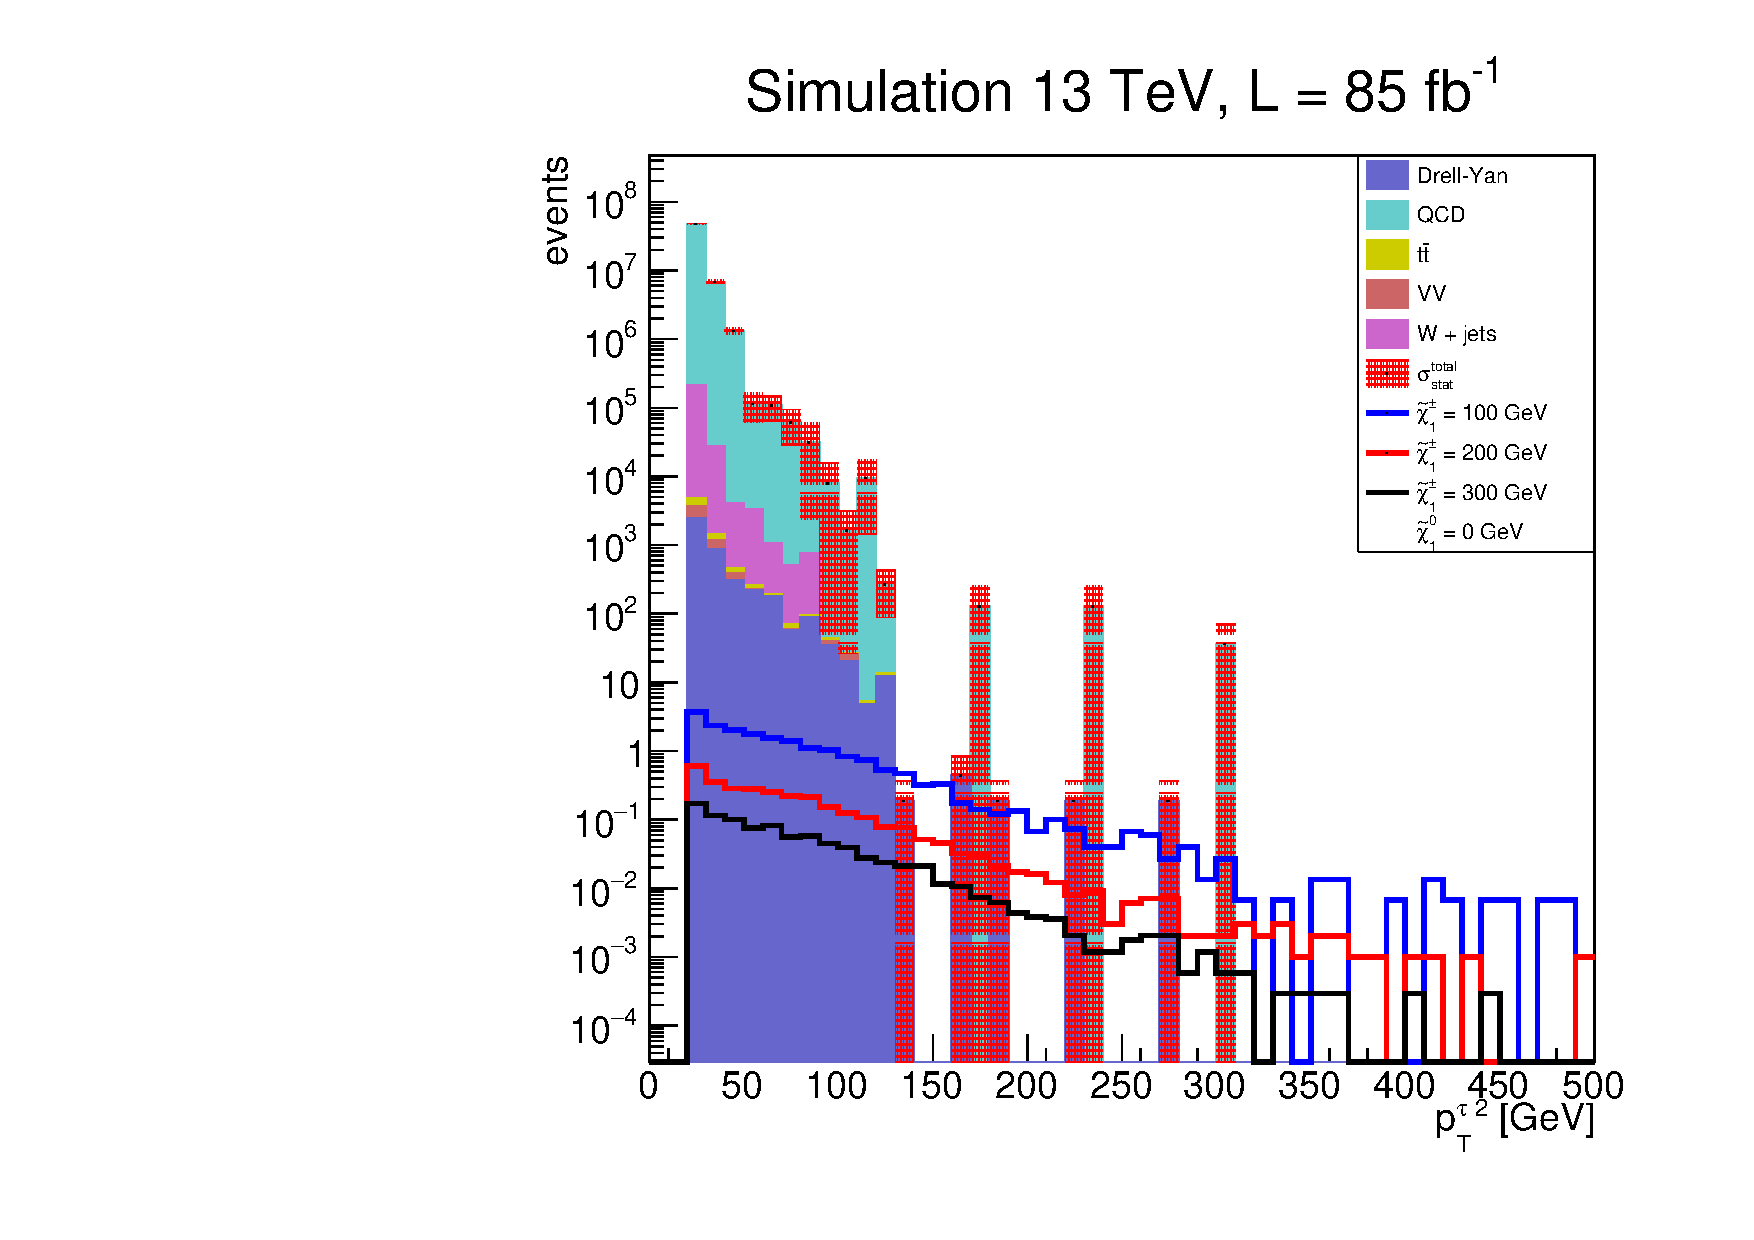
\includegraphics[width=0.5\textwidth]{analysis/pics/h_tau2pt_Tau2LooseIsoInclusiveVBFInverted.pdf}
	\end{tabular}
	\caption{(Left) Leading jet \pt distribution and (Right) and second leading \hadtau \pt distribution of selected signal and all MC background samples in control region 4.}
	\label{fig::crplots2_Tau2LooseIsoInclusiveVBFInverted_13tev}
\end{figure}

\clearpage

\section{Signal cross-section limits at 13 TeV}
\label{sec::xseclim_results}

This section shows the final results for the sensitivity study done on 13\tev simulated samples as function of the invariant mass of the di-jet candidate,  \met and the reconstructed \hadtau \pt. The different benchmark points were choses in term of different theoretical assumptions (fixed- and average-\stau-mass) and scenarios (uncompressed mass and compressed mass spectrum) for \charginopm and \neutralinoone masses of 100, 200, 300 400 and 500\gev. Given the trivial assumption that the cross section limit is strictly correlated to the reconstructed \hadtau \pt all the below results are shown considering a cut of 20\gev over this variable.

\todo{explain the table content, the limit plot and the cross section limit comparison}

\subsection*{Uncompressed scenario, fixed-\stau mass}

\FloatBarrier


\begin{figure}[tbh!]
	\centering
	\begin{tabular}{cc}
		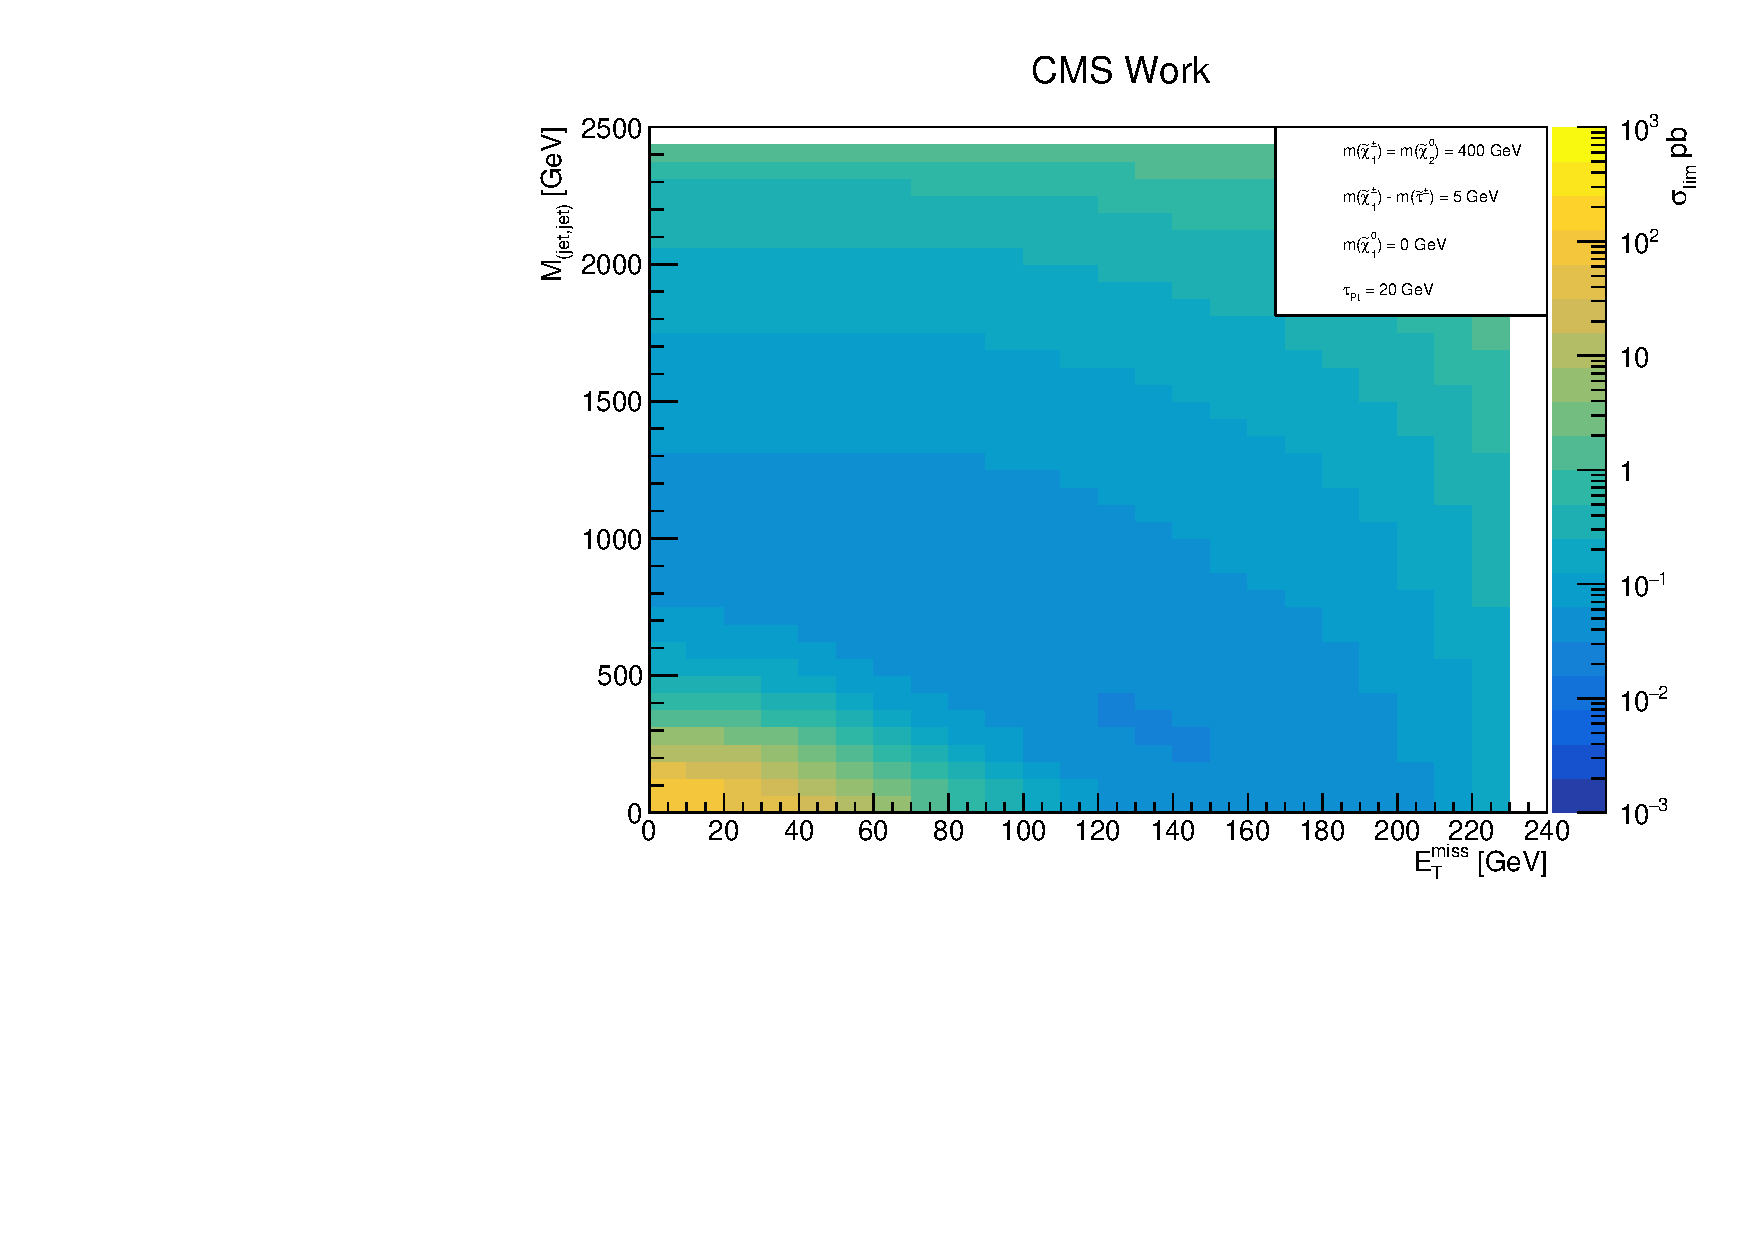
\includegraphics[width=0.75\textwidth]{analysis/pics/JetInvMass_vs_MET_xseclim_Chargino400_Stau395_LSP000_taupt20.pdf}
	\end{tabular}
	\caption{Cross section limit as function of $m_{jj}$ and \met for m(\charginopm) = m(\neutralinotwo) = 400 GeV,  m(\stau) = 395 GeV, and m(\neutralinoone) = 0 GeV and an offline selection on $\pt(\hadtau) <  20\gev$.}
	\label{fig::JetInvMass_vs_MET_xseclim_Chargino400_Stau395_LSP000_taupt20}
\end{figure}

\begin{table}
	\begin{center}
		
		\begin{tabular}{| c | c | c | c | }
			\toprule
			\multicolumn{4}{| c | }{m(\charginopm) = m(\stau) = 5\gev; m(\neutralinoone) = 0\gev} \\
			\midrule
			$\sigma_{lim}^{min}\pm(stat.)\pm(MC syst.)\pm(VBF syst.)$ [pb]  & m(\charginopm) = m(\neutralinotwo) [GeV] & \mjj [GeV] & \met [GeV] \\
			\midrule
			$0.033\pm0.002^{+0.003 + 0.001}_{-0.004-0.001}$ & $<$ 100 & $<$ 250  & $<$ 130 \\ 
			$0.033\pm0.002^{+0.003 + 0.001}_{-0.004-0.001}$ & $<$ 200 & $<$ 250  & $<$ 130 \\ 
			$0.034\pm0.002^{+0.003 + 0.001}_{-0.004-0.001}$ & $<$ 300 & $<$ 312.5  & $<$ 120 \\ 
			$0.030\pm0.001^{+0.002 + 0.001}_{-0.003-0.000}$ & $<$ 400 & $<$ 312.5  & $<$ 130 \\ 
			$0.030\pm0.001^{+0.003+ 0.001}_{-0.003-0.000}$ & $<$ 500 & $<$ 250  & $<$ 130 \\ 
			\bottomrule
		\end{tabular}\caption{Cross section limit minimum reached at the given cuts for $m_{jj}$, \met and an increasing \charginopm = \neutralinotwo for the uncompressed mass spectra and fixed-\stau mass  benchmark point.}
		\label{table::xseclim_uncompressed_fixedmass}
	\end{center}
\end{table}

\begin{figure}[tbh!]
	\centering
	\begin{tabular}{cc}
		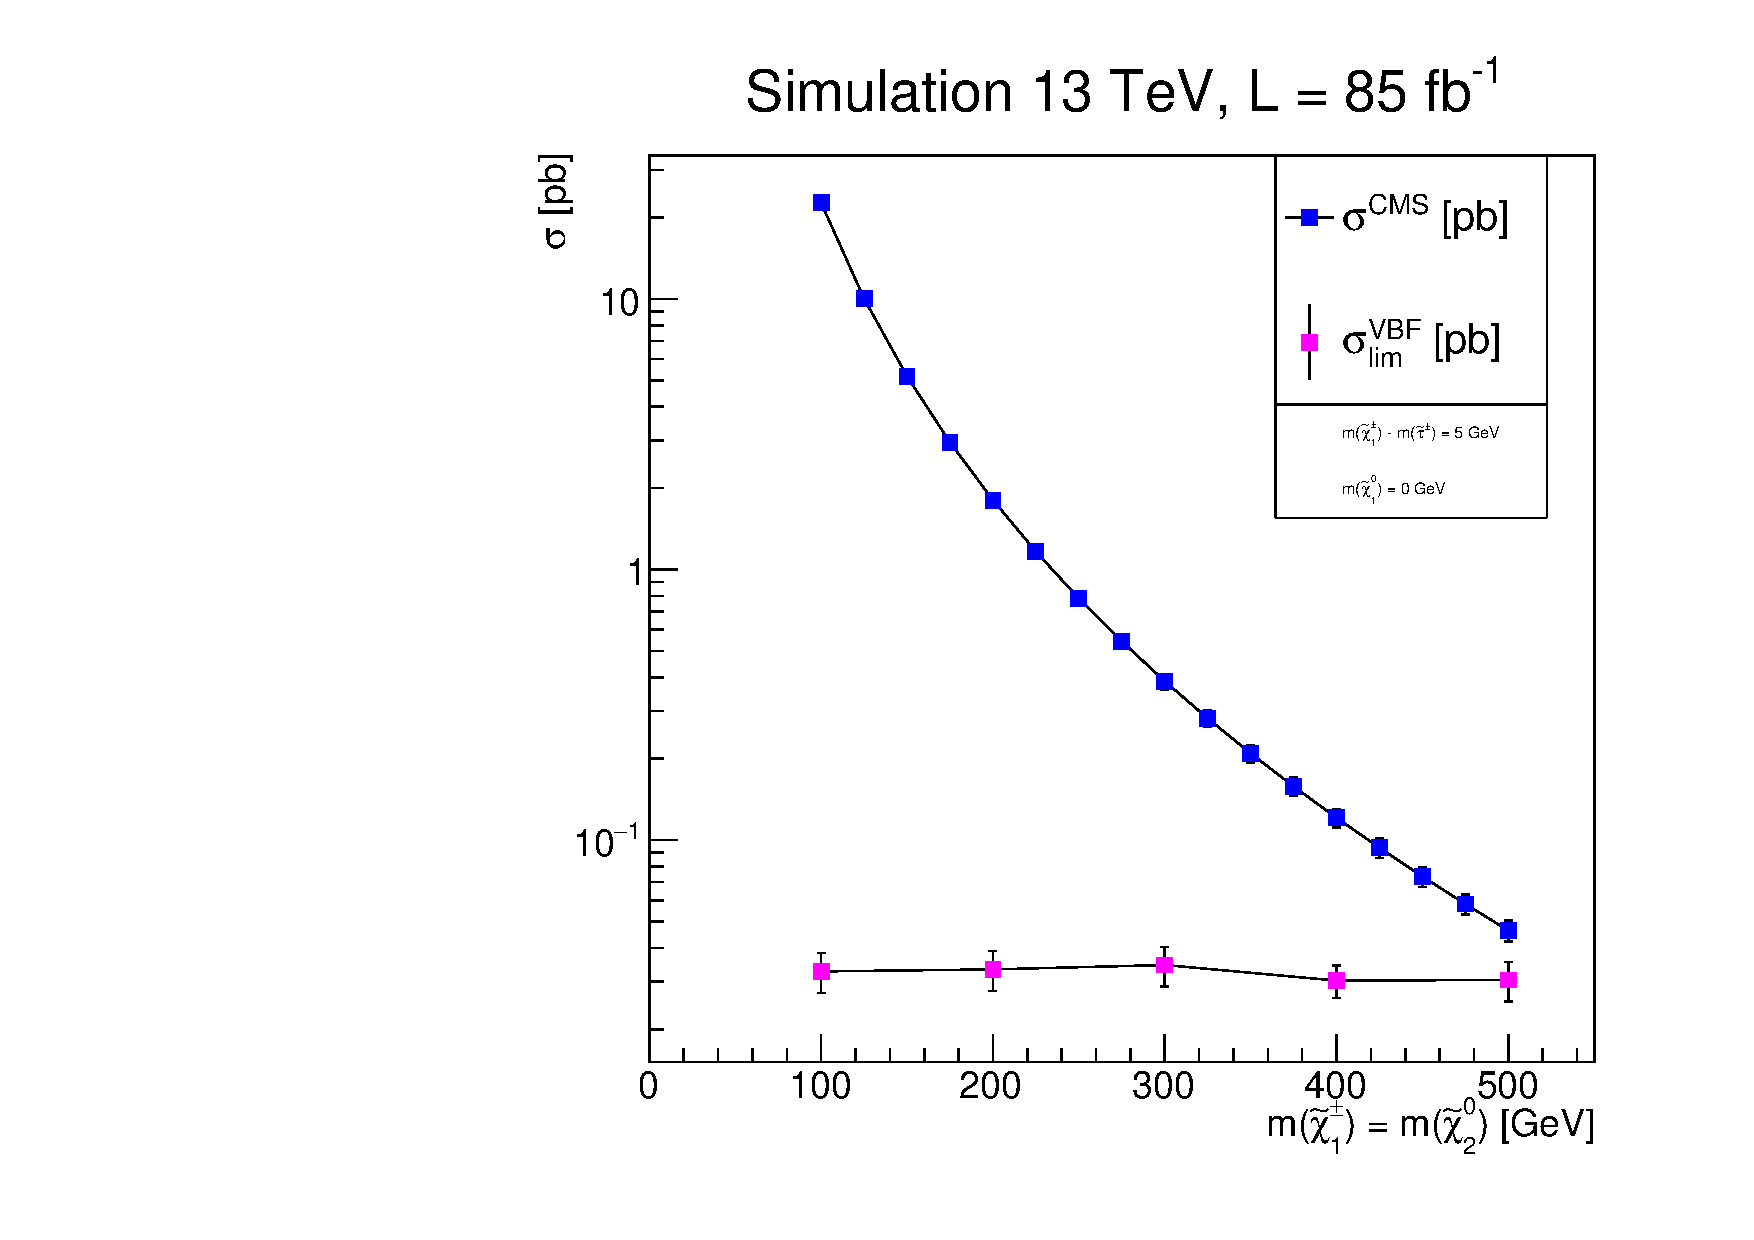
\includegraphics[width=0.75\textwidth]{analysis/pics/out_xsecmin_lsp000_stauclose.pdf}
	\end{tabular}
	\caption{Comparison between the cross section limit taken from the study over the uncompressed mass spectra and fixed-\stau mass benchmark point and the official CMS cross sections calculated using the \texttt{resummino} code from B. Fuks et al with CTEQ6.6 and MSTW2008nlo90cl PDFs \cite{Fuks:2013vua}.}
	\label{fig::out_xsecmin_lsp000_stauclose}
\end{figure}


\FloatBarrier

\subsection*{Compressed scenario, fixed-\stau mass}


\begin{figure}[tbh!]
	\centering
	\begin{tabular}{cc}
		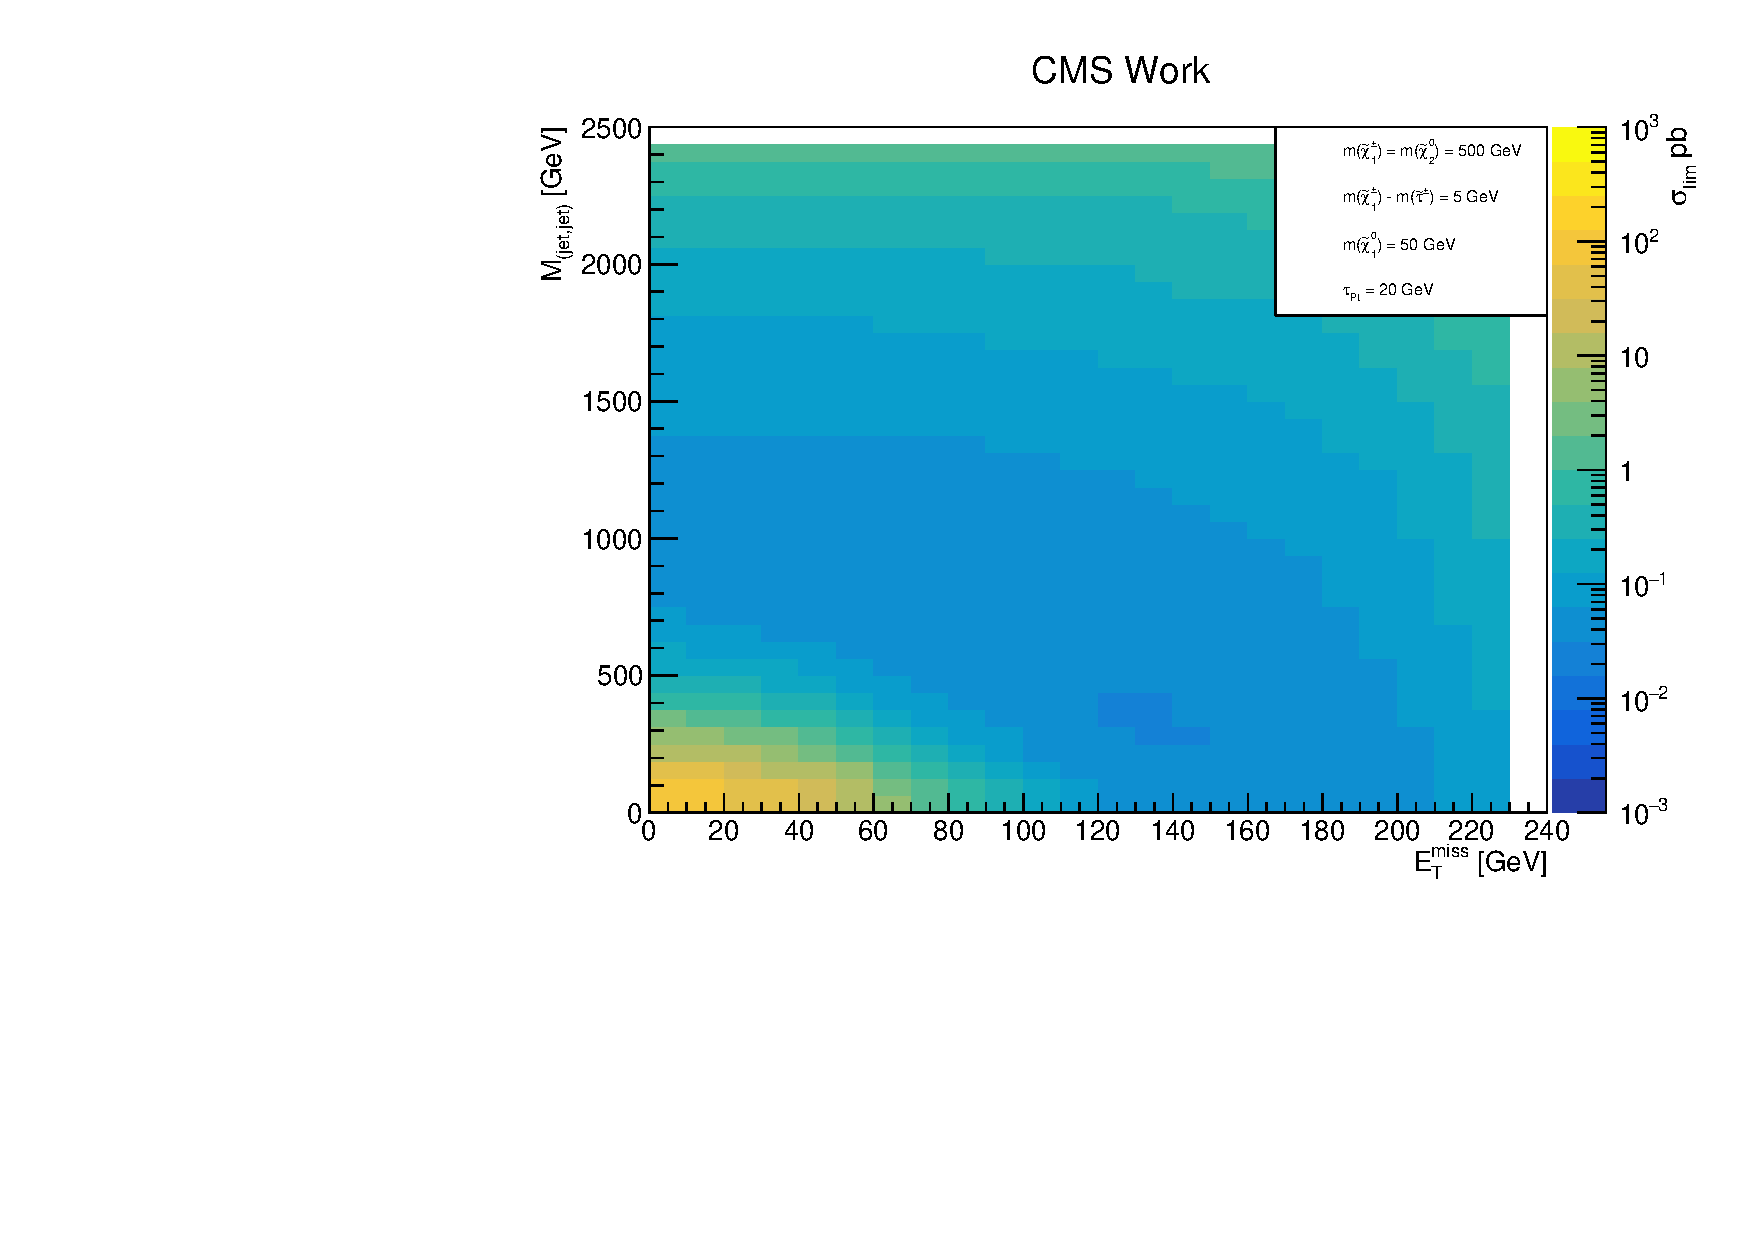
\includegraphics[width=0.75\textwidth]{analysis/pics/JetInvMass_vs_MET_xseclim_Chargino500_Stau495_LSP050_taupt20.pdf}
	\end{tabular}
	\caption{Cross section limit as function of $m_{jj}$ and \met for m(\charginopm) = m(\neutralinotwo) = 500 GeV,  m(\stau) = 495 GeV, and m(\neutralinoone) = 50 GeV and an offline selection on $\pt(\hadtau) <  20\gev$.}
	\label{fig::JetInvMass_vs_MET_xseclim_Chargino500_Stau495_LSP050_taupt20}
\end{figure}

\begin{table}
	\begin{center}
		
		\begin{tabular}{| c | c | c | c | }
			\toprule
			\multicolumn{4}{| c | }{m(\charginopm) = m(\stau) = 5\gev; m(\charginopm) - m(\neutralinoone) = 50\gev} \\
			\midrule
			$\sigma_{lim}^{min}\pm(stat.)\pm(MC syst.)\pm(VBF syst.)$ [pb]  & m(\charginopm) = m(\neutralinotwo) [GeV] & \mjj [GeV] & \met [GeV] \\
			\midrule
			$0.033\pm0.002^{+0.003 + 0.001}_{-0.004-0.001}$ & $<$ 100 & $<$ 250  & $<$ 130 \\ 
			$0.033\pm0.002^{+0.003 + 0.001}_{-0.004-0.001}$ & $<$ 200 & $<$ 312.5  & $<$ 120 \\ 
			$0.033\pm0.001^{+0.002 + 0.001}_{-0.003-0.000}$ & $<$ 300 & $<$ 312.5  & $<$ 130 \\ 
			$0.031\pm0.001^{+0.002 + 0.001}_{-0.003-0.001}$ & $<$ 400 & $<$ 250  & $<$ 130 \\ 
			$0.030\pm0.001^{+0.002 + 0.001}_{-0.003-0.000}$ & $<$ 500 & $<$ 312.5  & $<$ 130 \\ 
			\bottomrule
		\end{tabular}\caption{Cross section limit minimum reached at the given cuts for $m_{jj}$, \met and an increasing \charginopm = \neutralinotwo for the compressed mass spectra and fixed-\stau mass  benchmark point.}
		\label{table::xseclim_compressed_fixedmass}
	\end{center}
\end{table}

\begin{figure}[tbh!]
	\centering
	\begin{tabular}{cc}
		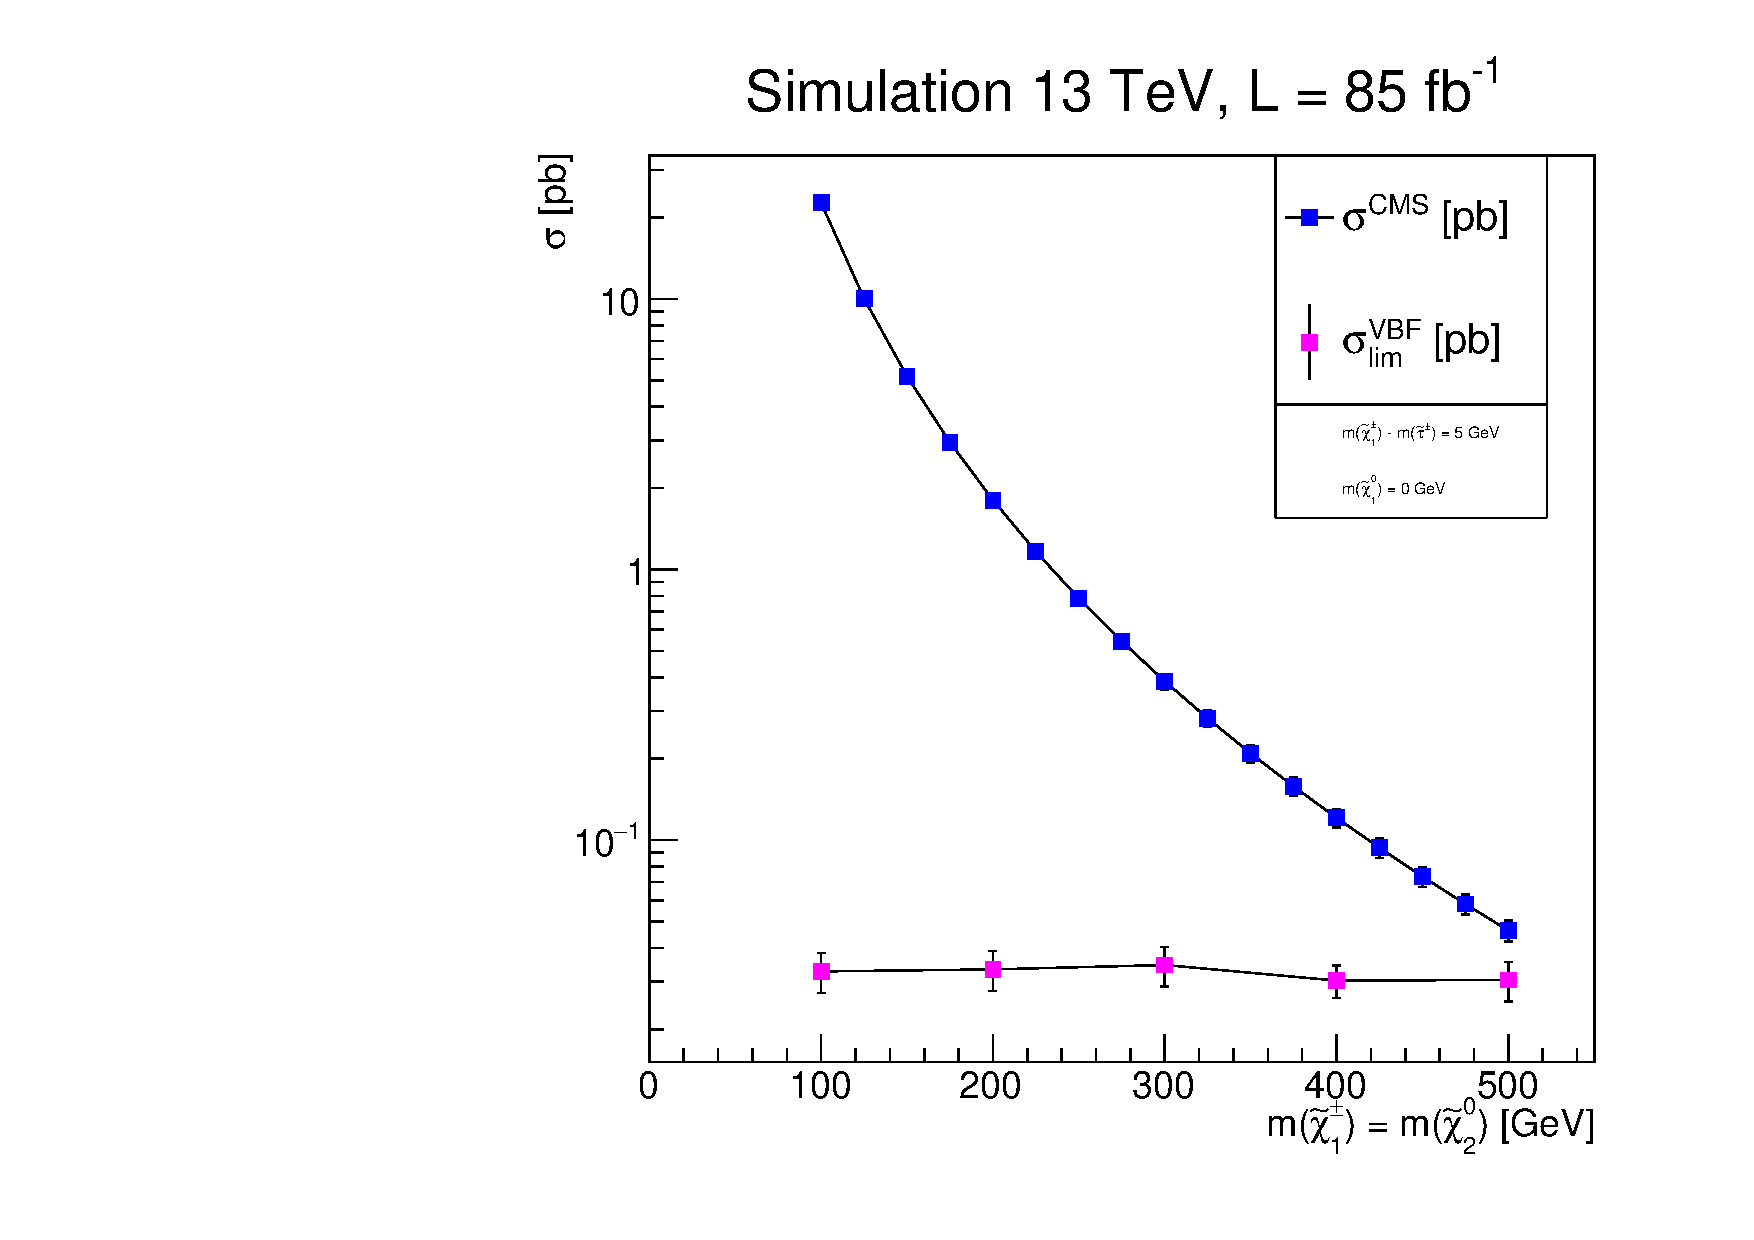
\includegraphics[width=0.75\textwidth]{analysis/pics/out_xsecmin_lsp000_stauclose.pdf}
	\end{tabular}
	\caption{Comparison between the cross section limit taken from the study over the compressed mass spectra and fixed-\stau mass benchmark point and the official CMS cross sections calculated using the \texttt{resummino} code from B. Fuks et al with CTEQ6.6 and MSTW2008nlo90cl PDFs \cite{Fuks:2013vua}.}
	\label{fig::out_xsecmin_lsp050_stauclose}
\end{figure}


\FloatBarrier

\subsection*{Uncompressed scenario, average-\stau mass}


\begin{figure}[tbh!]
	\centering
	\begin{tabular}{cc}
		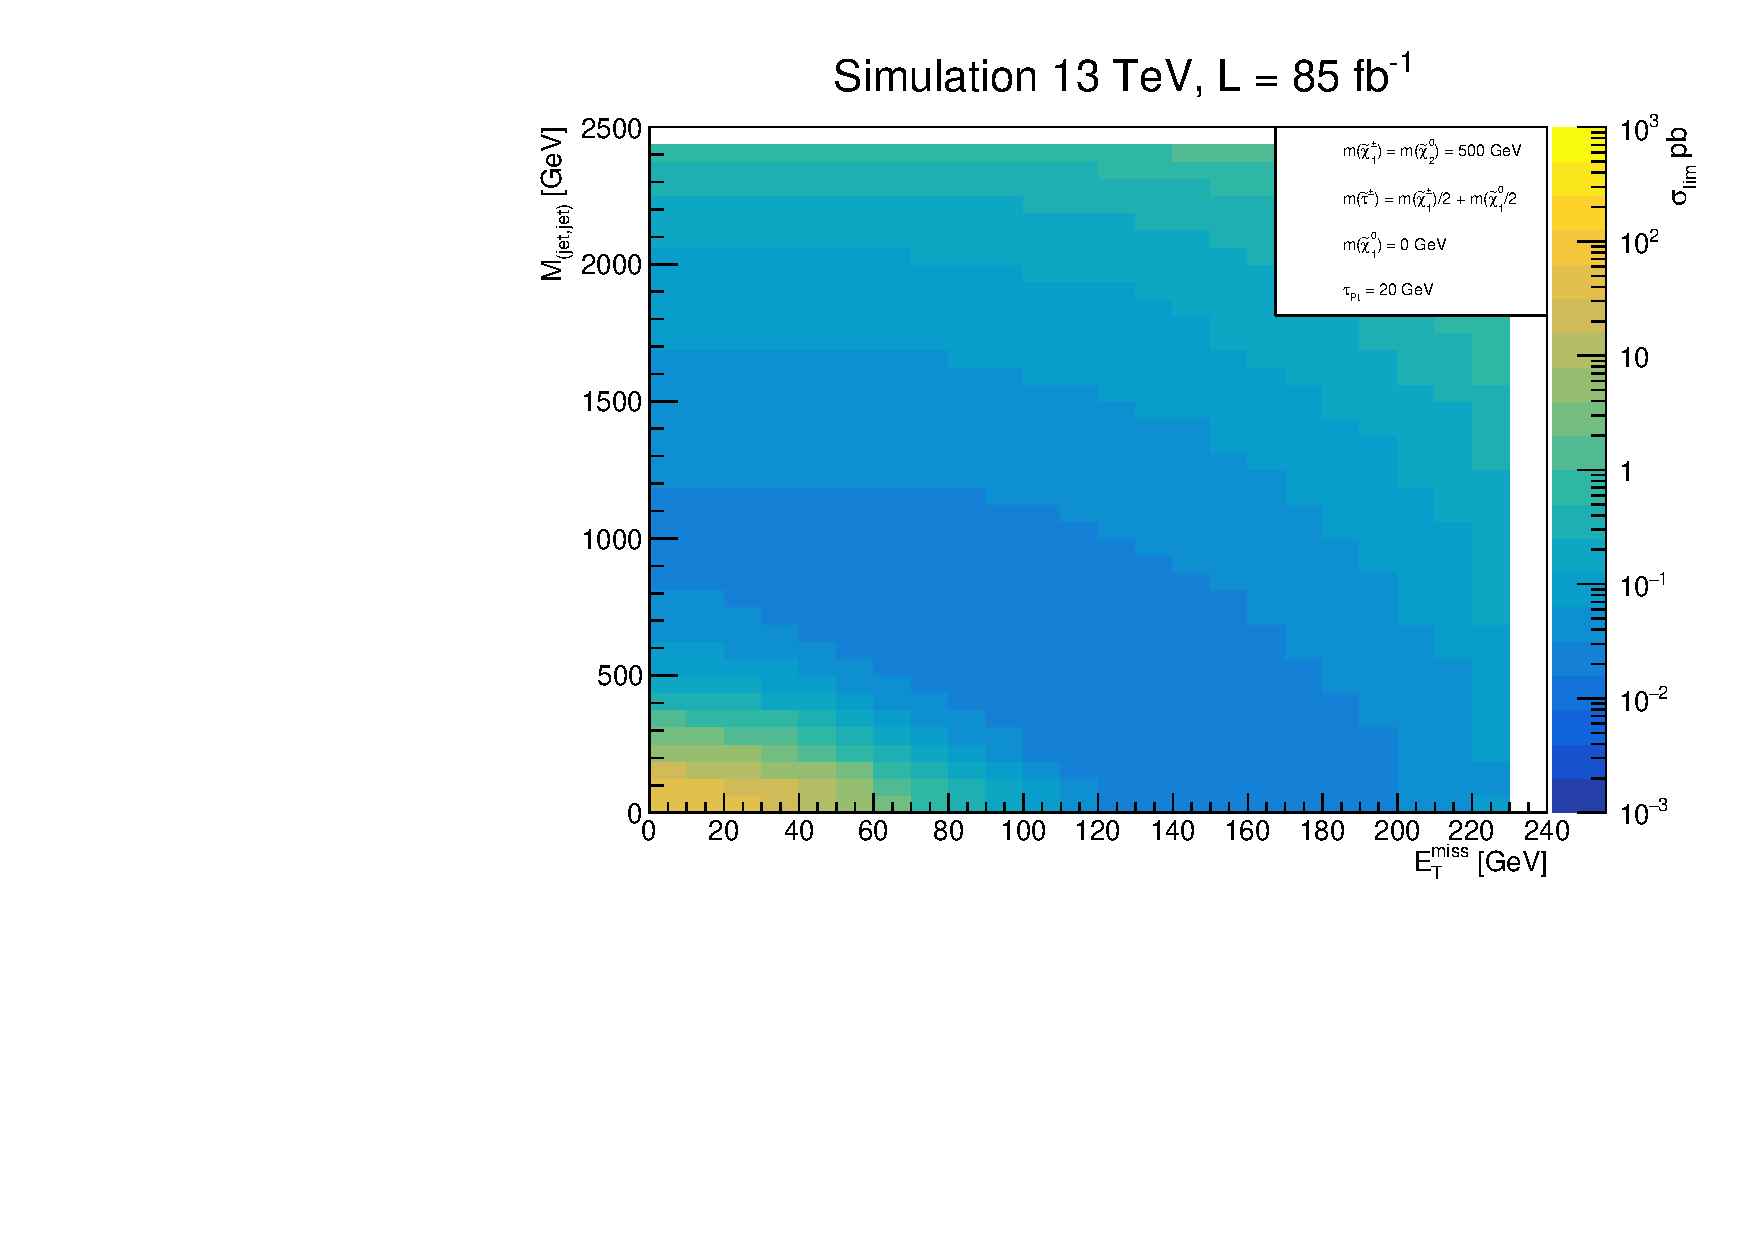
\includegraphics[width=0.75\textwidth]{analysis/pics/JetInvMass_vs_MET_xseclim_Chargino500_Stau250_LSP000_taupt20.pdf}
	\end{tabular}
	\caption{Cross section limit as function of $m_{jj}$ and \met for m(\charginopm) = m(\neutralinotwo) = 500 GeV,  m(\stau) = 250 GeV, and m(\neutralinoone) = 0 GeV and an offline selection on $\pt(\hadtau) <  20\gev$.}
	\label{fig::JetInvMass_vs_MET_xseclim_Chargino500_Stau250_LSP000_taupt20}
\end{figure}

\begin{table}
	\begin{center}
		
		\begin{tabular}{| c | c | c | c | }
			\toprule
			\multicolumn{4}{| c | }{m(\stau) = 0.5 m(\neutralinoone) + 0.5 m(\charginopm) ; m(\neutralinoone) = 0\gev} \\
			\midrule
			$\sigma_{lim}^{min}\pm(stat.)\pm(MC syst.)\pm(VBF syst.)$ [pb]  & m(\charginopm) = m(\neutralinotwo) [GeV] & \mjj [GeV] & \met [GeV] \\
			\midrule
				$0.083\pm0.005^{+0.007 + 0.003}_{-0.009-0.001}$ & $<$ 100 & $<$ 312.5  & $<$ 120 \\ 
				$0.036\pm0.002^{+0.003 + 0.001}_{-0.004-0.001}$ & $<$ 200 & $<$ 375  & $<$ 110 \\ 
				$0.024\pm0.001^{+0.002 + 0.001}_{-0.003-0.000}$ & $<$ 300 & $<$ 250  & $<$ 130 \\ 
				$0.019\pm0.001^{+0.002 + 0.001}_{-0.002-0.000}$ & $<$ 400 & $<$ 250  & $<$ 130 \\ 
				$0.017\pm0.001^{+0.002 + 0.001}_{-0.002-0.000}$ & $<$ 500 & $<$ 250  & $<$ 130 \\ 
			\bottomrule
		\end{tabular}\caption{Cross section limit minimum reached at the given cuts for $m_{jj}$, \met and an increasing \charginopm = \neutralinotwo for the uncompressed mass spectra and average-\stau mass benchmark point.}
		\label{table::xseclim_uncompressed_averagemass}
	\end{center}
\end{table}

\begin{figure}[tbh!]
	\centering
	\begin{tabular}{cc}
		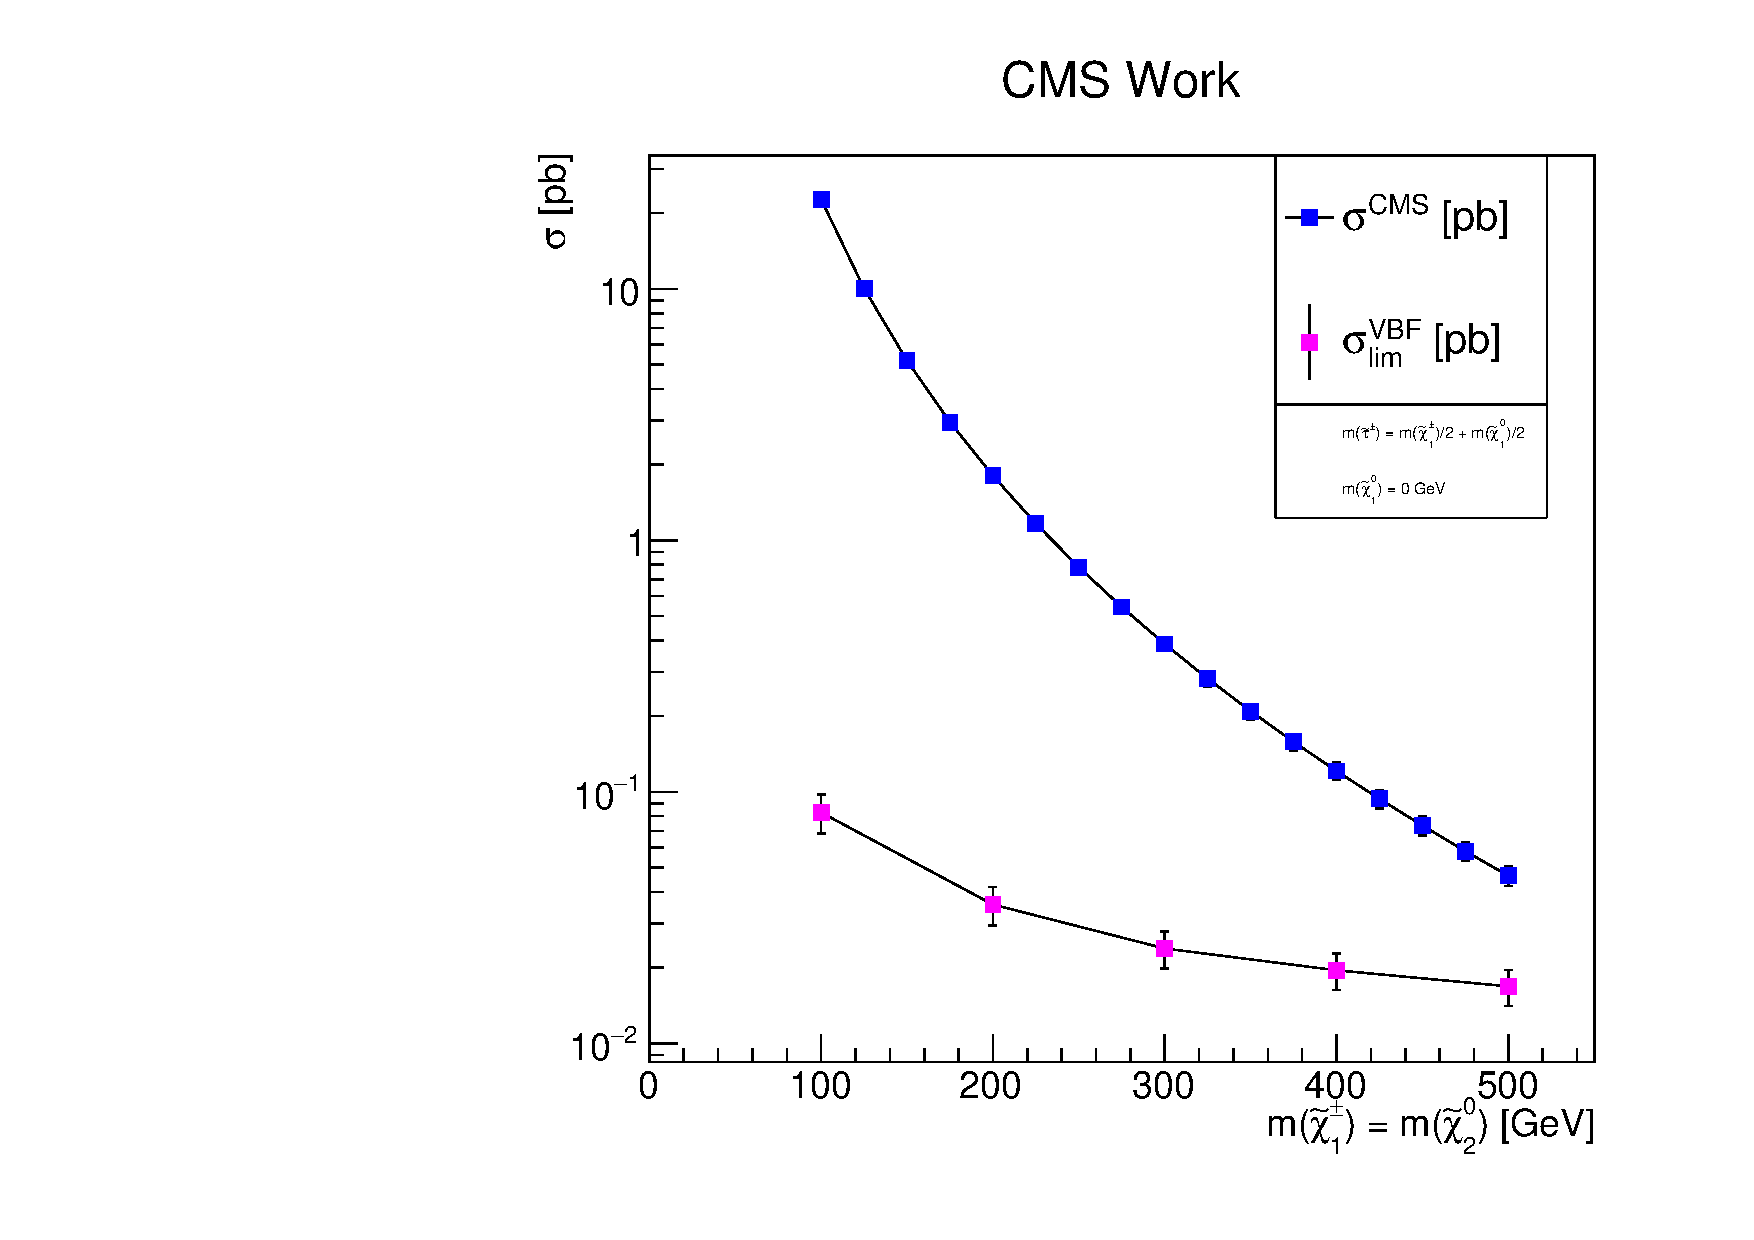
\includegraphics[width=0.75\textwidth]{analysis/pics/out_xsecmin_lsp000_staufar.pdf}
	\end{tabular}
	\caption{Comparison between the cross section limit taken from the study over the uncompressed mass spectra and average-\stau mass benchmark point and the official CMS cross sections calculated using the \texttt{resummino} code from B. Fuks et al with CTEQ6.6 and MSTW2008nlo90cl PDFs \cite{Fuks:2013vua}.}
	\label{fig::out_xsecmin_lsp000_staufar}
\end{figure}

\FloatBarrier

\subsection*{Compressed scenario, average-\stau mass}


\begin{figure}[tbh!]
	\centering
	\begin{tabular}{cc}
		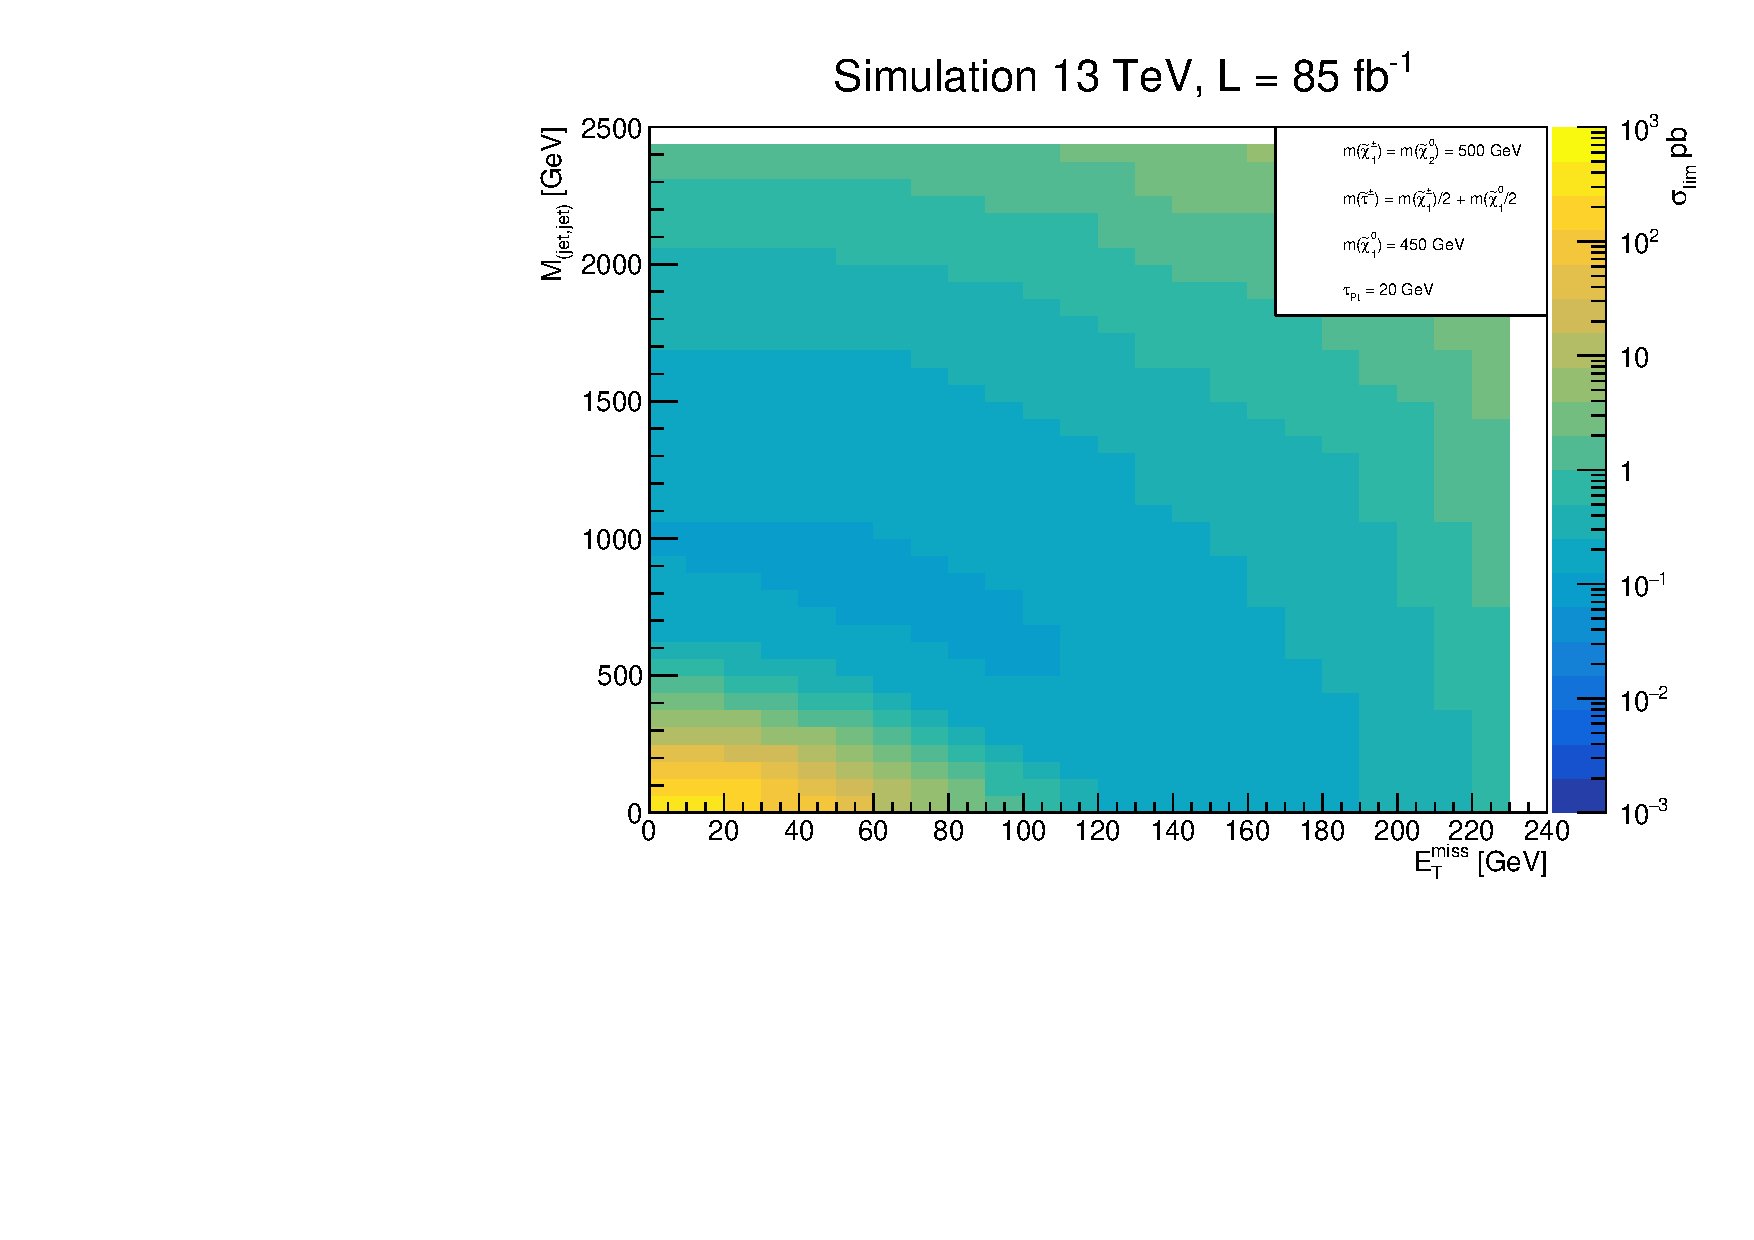
\includegraphics[width=0.75\textwidth]{analysis/pics/JetInvMass_vs_MET_xseclim_Chargino500_Stau475_LSP450_taupt20.pdf}
	\end{tabular}
	\caption{Cross section limit as function of $m_{jj}$ and \met for m(\charginopm) = m(\neutralinotwo) = 500 GeV,  m(\stau) = 475 GeV, and m(\neutralinoone) = 450 GeV and an offline selection on $\pt(\hadtau) <  20\gev$.}
	\label{fig::JetInvMass_vs_MET_xseclim_Chargino500_Stau475_LSP450_taupt20}
\end{figure}

\begin{table}
	\begin{center}
		
		\begin{tabular}{| c | c | c | c | }
			\toprule
			\multicolumn{4}{| c | }{m(\stau) = 0.5 m(\neutralinoone) + 0.5 m(\charginopm) ; m(\charginopm) - m(\neutralinoone) = 50\gev} \\
			\midrule
			$\sigma_{lim}^{min}\pm(stat.)\pm(MC syst.)\pm(VBF syst.)$ [pb]  & m(\charginopm) = m(\neutralinotwo) [GeV] & \mjj [GeV] & \met [GeV] \\
			\midrule
				$0.153\pm0.011^{+0.012 + 0.005}_{-0.014-0.002}$ & $<$ 100 & $<$ 500  & $<$ 100 \\ 
				$0.148\pm0.011^{+0.014 + 0.005}_{-0.017-0.002}$ & $<$ 200 & $<$ 375  & $<$ 110 \\ 
				$0.157\pm0.011^{+0.013 + 0.005}_{-0.015-0.002}$ & $<$ 300 & $<$ 562.5  & $<$ 90 \\ 
				$0.150\pm0.011^{+0.014 + 0.005}_{-0.016-0.002}$ & $<$ 400 & $<$ 312.5  & $<$ 120 \\ 
				$0.115\pm0.007^{+0.010 + 0.004}_{-0.012-0.002}$ & $<$ 500 & $<$ 750  & $<$ 60 \\
			\bottomrule
		\end{tabular}\caption{Cross section limit minimum reached at the given cuts for $m_{jj}$, \met and an increasing \charginopm = \neutralinotwo for the compressed mass spectra and average-\stau mass benchmark point.}
		\label{table::xseclim_compressed_averagemass}
	\end{center}
\end{table}

\begin{figure}[tbh!]
	\centering
	\begin{tabular}{cc}
		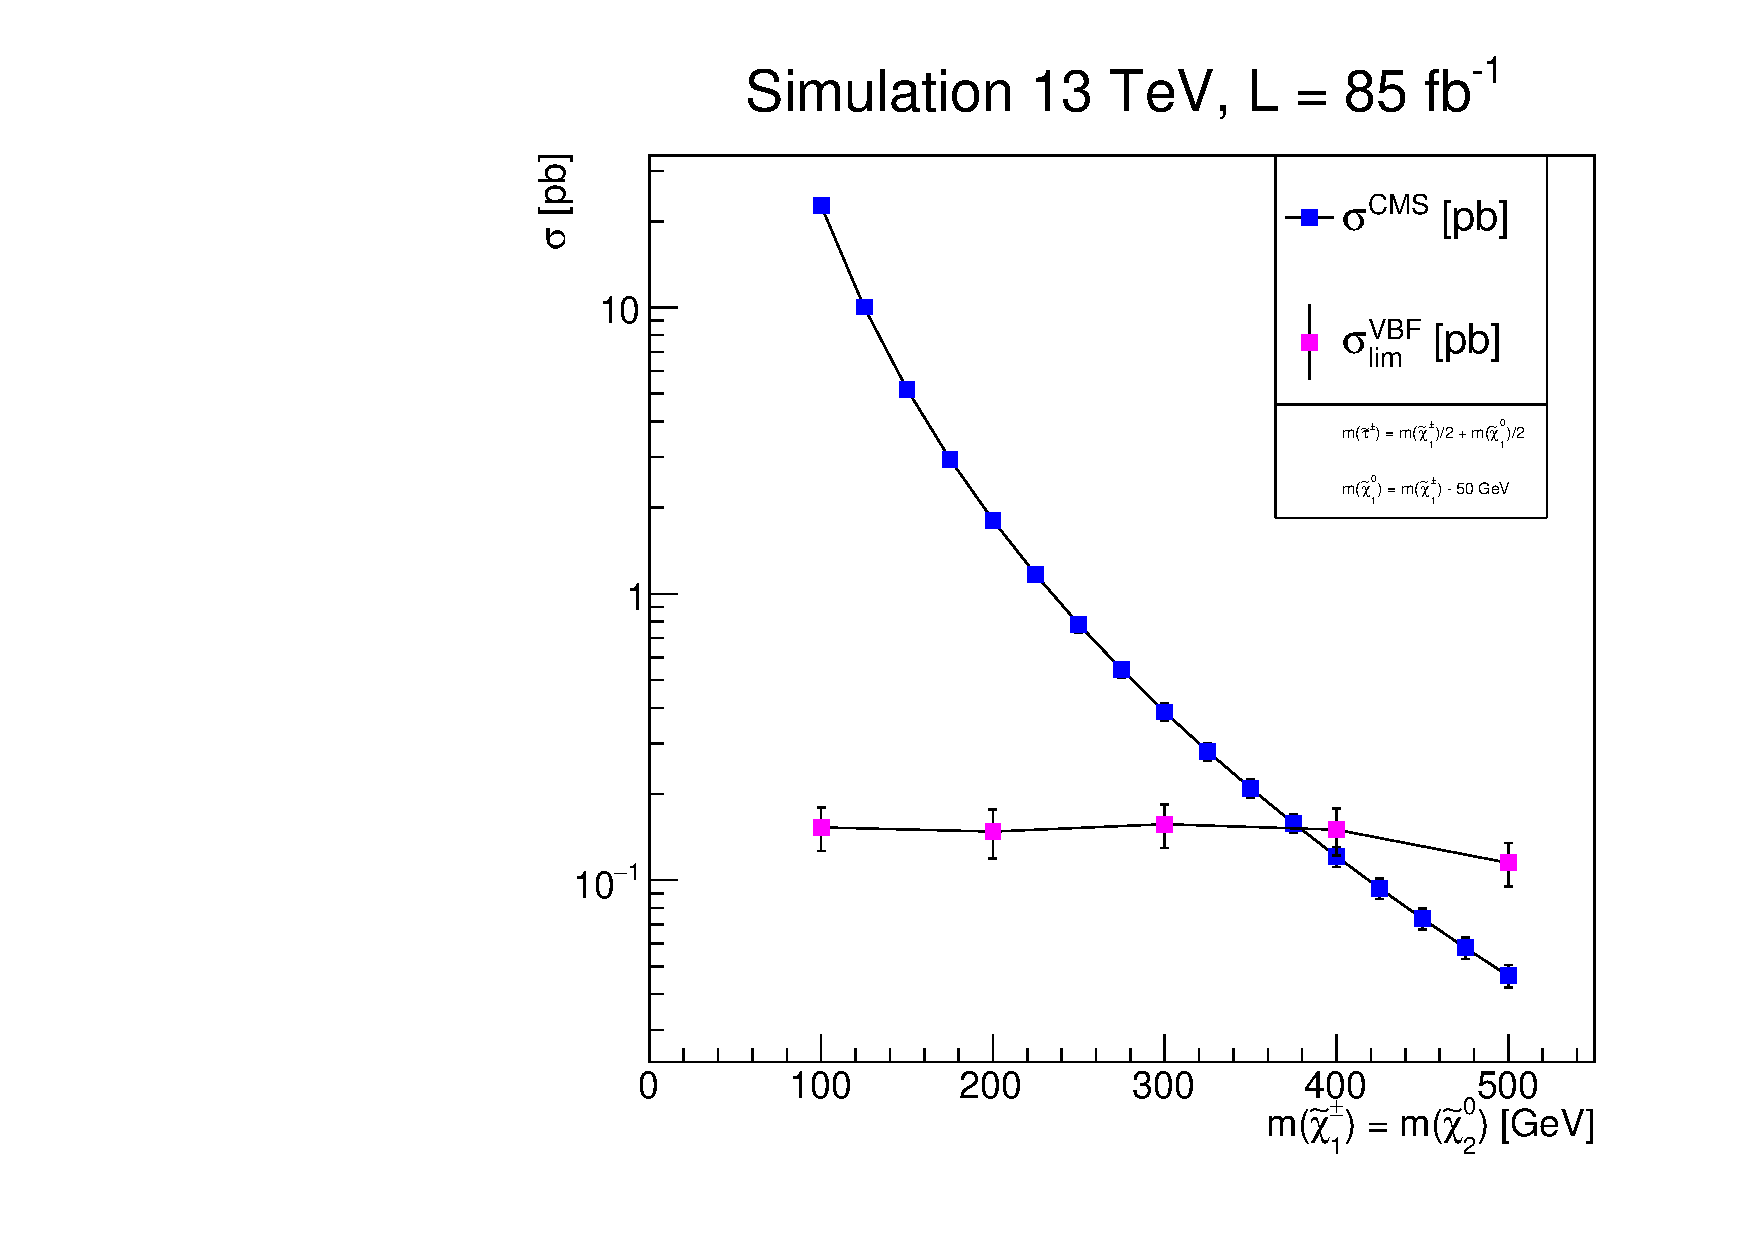
\includegraphics[width=0.75\textwidth]{analysis/pics/out_xsecmin_lspcomp_stauclose.pdf}
	\end{tabular}
	\caption{Comparison between the cross section limit taken from the study over the compressed mass spectra and average-\stau mass benchmark point and the official CMS cross sections calculated using the \texttt{resummino} code from B. Fuks et al with CTEQ6.6 and MSTW2008nlo90cl PDFs \cite{Fuks:2013vua}.}
	\label{fig::out_xsecmin_lspcomp_stauclose}
\end{figure}

\FloatBarrier

